\documentclass[11pt,a4paper]{article}
\usepackage[T1]{fontenc}
\usepackage[utf8]{inputenc}
\usepackage{lmodern}
\usepackage[margin=18mm]{geometry}
\usepackage{enumitem,xcolor,fancyhdr,array,tabularx,booktabs,amsmath,amssymb,tikz}
\definecolor{slate}{HTML}{2F3E4E}
\definecolor{ember}{HTML}{C8501E}
\definecolor{codebg}{HTML}{F3F5F7}
\usepackage[colorlinks=true,linkcolor=slate,urlcolor=ember]{hyperref}
\hypersetup{bookmarksdepth=2}
\setcounter{tocdepth}{1}
% contents lines: a wider number column (for "10") and tighter spacing between chapters
\makeatletter
\renewcommand*\l@section[2]{%
  \ifnum \c@tocdepth >\z@
    \addpenalty\@secpenalty
    \addvspace{0.5em \@plus\p@}%
    \setlength\@tempdima{2.2em}%
    \begingroup
      \parindent \z@ \rightskip \@pnumwidth
      \parfillskip -\@pnumwidth
      \leavevmode \bfseries
      \advance\leftskip\@tempdima
      \hskip -\leftskip
      #1\nobreak\hfil \nobreak\hb@xt@\@pnumwidth{\hss #2}\par
    \endgroup
  \fi}
\makeatother
\pagestyle{fancy}\fancyhf{}
\lhead{\small\color{slate}Aptitude notes}
\rhead{\small\color{slate}Page \thepage}
\setlength{\parindent}{0pt}
\setlength{\parskip}{5pt}
\setlength{\emergencystretch}{3em}
\sloppy
\setlist{itemsep=2pt,topsep=3pt,leftmargin=*}
\usepackage{titlesec}
\titleformat{\section}{\Large\bfseries\color{ember}}{\thesection}{0.6em}{}[{\color{slate}\titlerule}]
\titleformat{\subsection}{\large\bfseries\color{slate}}{\thesubsection}{0.6em}{}
\titleformat{name=\subsection,numberless}{\large\bfseries\color{slate}}{}{0em}{}
\titleformat{name=\section,numberless}{\Large\bfseries\color{ember}}{}{0em}{}[{\color{slate}\titlerule}]
% keep a type heading together with its first lines (no heading stranded at a page bottom)
\usepackage{needspace,multicol}
\let\oldsubsection\subsection
\renewcommand{\subsection}{\needspace{9\baselineskip}\oldsubsection}

% ---- block labels (copy a whole type block to add a new type) ----
\newcommand{\spot}{\textbf{\color{ember}Spot it.}\ }
\newcommand{\mech}{\textbf{\color{ember}Mechanism.}\ }
% \keepsamptrue (set before a chapter) keeps each Sample line together with its first working lines
\newif\ifkeepsamp
\keepsamptrue
\newcommand{\ans}[1]{\par\nopagebreak\noindent\textbf{\color{ember}Answer:}\ \textbf{#1}\par}
\newcommand{\samp}{\ifkeepsamp\needspace{4\baselineskip}\fi\textbf{\color{ember}Sample.}\ }
\newcommand{\sane}{\textbf{\color{slate}Sanity check.}\ }
\newcommand{\tryit}[1]{\textbf{\color{ember}Try it.}\ #1}
\newcommand{\infobox}[2]{\par\medskip\noindent\begingroup\setlength{\fboxsep}{7pt}%
  \colorbox{codebg}{\parbox{\dimexpr\linewidth-14pt\relax}{\textbf{\color{ember}#1}\par\smallskip #2}}\endgroup\par\medskip}

% family-tree boxes (blood relations): square corners = man, rounded = woman, dashed = either
\tikzset{
  man/.style={rectangle,draw=slate,thick,fill=white,minimum width=19mm,minimum height=7.5mm,align=center,inner sep=2pt,font=\scriptsize},
  woman/.style={rectangle,rounded corners=3.5mm,draw=ember,thick,fill=white,minimum width=19mm,minimum height=7.5mm,align=center,inner sep=2pt,font=\scriptsize},
  anyone/.style={rectangle,rounded corners=1.2mm,draw=slate!70,dashed,thick,fill=white,minimum width=19mm,minimum height=7.5mm,align=center,inner sep=2pt,font=\scriptsize}}

\begin{document}
\begin{center}
{\LARGE\bfseries\color{slate}Aptitude notes}\\[3pt]
{\color{ember}Quantitative aptitude and reasoning: shortcuts you can spot, apply and check}
\end{center}
\section*{Chapters at a glance}
\begin{center}\small\renewcommand{\arraystretch}{1.3}\setlength{\tabcolsep}{6pt}
\begin{tabularx}{\linewidth}{@{}r >{\raggedright\arraybackslash}p{3.9cm} l >{\raggedright\arraybackslash}X r@{}}
\toprule
\textbf{\color{slate}No.} & \textbf{\color{slate}Chapter} & \textbf{\color{slate}Types} & \textbf{\color{slate}The one idea} & \textbf{\color{slate}Page} \\ \midrule
\multicolumn{5}{@{}l}{\textbf{\color{ember}Quantitative aptitude}} \\
\ref{ch:T} & Time and work & T1--T12 & total work is the LCM of the days (chairs); add the rates & \pageref{ch:T} \\
\ref{ch:S} & Speed, distance and time & S1--S12 & $D = S \times T$; pick a convenient distance; add or subtract speeds & \pageref{ch:S} \\
\ref{ch:P} & Percentages & P1--P12 & percent of what? Start from 100 & \pageref{ch:P} \\
\ref{ch:R} & Ratio and proportion & R1--R12 & find what one part is worth & \pageref{ch:R} \\
\ref{ch:M} & Mixtures and alligation & M1--M12 & the mean sits between; quantities go opposite to the gaps & \pageref{ch:M} \\
\ref{ch:L} & Profit and loss & L1--L12 & profit and loss are out of the cost, a discount is out of the marked price & \pageref{ch:L} \\
\ref{ch:C} & Calendar & C1--C12 & only the odd days (what is left after whole weeks) matter & \pageref{ch:C} \\
\ref{ch:K} & Clocks & K1--K12 & 60 minute spaces; the minute hand gains $\frac{11}{12}$ of a space a minute & \pageref{ch:K} \\
\ref{ch:A} & Averages and ages & A1--A12 & work with totals; the age difference never changes & \pageref{ch:A} \\
\ref{ch:I} & Interest & I1--I12 & simple interest adds the same amount each year; compound interest multiplies by $1+\text{rate}$ each year & \pageref{ch:I} \\
\ref{ch:N} & Number series & N1--N12 & look at the differences first, then the ratios, then squares, cubes and primes & \pageref{ch:N} \\
\midrule
\multicolumn{5}{@{}l}{\textbf{\color{ember}Reasoning}} \\
\ref{ch:Y} & Syllogisms & Y1--Y12 & a conclusion follows only if it is true in every picture you can draw & \pageref{ch:Y} \\
\ref{ch:D} & Directions & D1--D12 & draw it with north at the top; turn every left and right into a compass direction; add each axis separately & \pageref{ch:D} \\
\ref{ch:B} & Blood relations & B1--B12 & draw the family tree; name a relative by generation, side and sex & \pageref{ch:B} \\
\bottomrule
\end{tabularx}\end{center}

\section*{How to read this file}
A revision file for quantitative aptitude and reasoning shortcuts. Every type, in every chapter, has the same four lines: \spot the wording that gives it away; \mech what to do, in plain steps; \textbf{\color{ember}Sample.}\ one solved example, one step per line, ending in a bold answer; \tryit{one question for you, with answers and working at the end of the chapter.} Each chapter has its own letter (T, S, P, R, M, L, C, K, A, I, N, Y, D, B) and numbers are never reused, so ``T7'' always means the same thing. In the PDF's sidebar every chapter opens into its types.

Chapter 1 introduces the \textbf{chair method}: the LCM of the days is the total number of chairs, and each person makes some chairs a day. The later chapters reuse the habit of choosing a convenient number: a distance, 100, parts, minute spaces, totals. The reasoning chapters swap numbers for pictures. More chapters will follow.

\clearpage
\section[Time and work (T1--T12)]{Time and work (with pipes and wages)}\label{ch:T}
\addtocontents{toc}{\protect\nopagebreak}

\subsection*{The one idea}
Think of the job as an order of chairs.

The question gives you days. It does not say how many chairs the job is. So you choose the number: take the LCM of the days. That is the total number of chairs.

Now each person makes a whole number of chairs a day. There are no fractions. This is the chair method.

\begin{center}
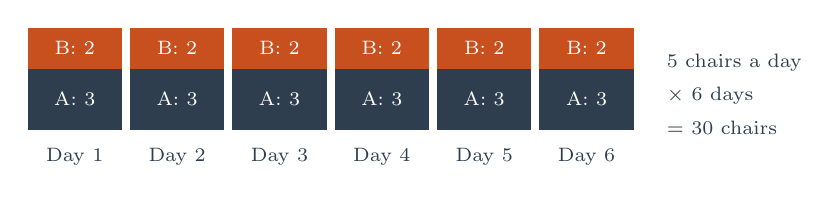
\begin{tikzpicture}[x=1.3cm,y=0.26cm,font=\scriptsize]
\foreach \dy in {0,...,5}{
  \fill[slate] (\dy,0) rectangle (\dy+0.92,3);
  \fill[ember] (\dy,3) rectangle (\dy+0.92,5);
  \node[white] at (\dy+0.46,1.5) {A: 3};
  \node[white] at (\dy+0.46,4) {B: 2};
  \pgfmathtruncatemacro{\dn}{\dy+1}
  \node[color=slate] at (\dy+0.46,-1.3) {Day \dn};
}
\node[anchor=west,color=slate] at (6.15,3.3) {5 chairs a day};
\node[anchor=west,color=slate] at (6.15,1.7) {$\times$ 6 days};
\node[anchor=west,color=slate] at (6.15,0.1) {= 30 chairs};
\end{tikzpicture}\par\nopagebreak\smallskip
{\small A takes 10 days. B takes 15 days. Total = LCM = 30 chairs. A makes 3 chairs a day and B makes 2. Together they make 5 a day, so the job takes 6 days.}
\end{center}

\infobox{The chair method in four steps (it solves almost every type below)}{
\begin{enumerate}
\item \textbf{Total chairs} = LCM of all the days (or hours) in the question.
\item \textbf{Chairs a day} for each person = total chairs $\div$ that person's days.
\item \textbf{Working together:} add their chairs a day. Subtract a leak or an outlet.
\item \textbf{Time} = chairs still to make $\div$ chairs made a day.
\end{enumerate}}

\subsection*{Spot-it table}
Read the wording, find the row, jump to the type.
\begin{center}\small\renewcommand{\arraystretch}{1.18}\setlength{\tabcolsep}{7pt}
\begin{tabularx}{\linewidth}{@{}>{\raggedright\arraybackslash}X l >{\raggedright\arraybackslash}X@{}}
\toprule
\textbf{\color{slate}Wording in the question} & \textbf{\color{slate}Type} & \textbf{\color{slate}The one move} \\ \midrule
X alone, Y alone, together? & T1 & add the chairs a day \\
Together they take..., A alone takes..., B alone? & T2 & team minus the known person \\
A and B, B and C, C and A take...; all three? & T3 & add the three pairs, then halve \\
Pipe fills, outlet or leak empties & T4 & the outlet is a minus \\
Fills in 6 h, but with a leak 8 h & T5 & leak = pipe minus net \\
A leaves (or B joins) after $d$ days & T6 & chairs made first, then the rest \\
Leaves $d$ days before the work ends & T7 & call the total time $T$ \\
Alternate days, in turns & T8 & count 2-day cycles, then the last days \\
Twice as efficient, 25\% more efficient & T9 & ratio of rates, flip it for days \\
$m$ men, $d$ days, $h$ hours a day & T10 & count the work in man-hours \\
Completes $3/5$ of the job in 12 days & T11 & find the time for one part \\
Paid Rs.\ 3000, share of each? & T12 & share by chairs made \\
\bottomrule
\end{tabularx}\end{center}

\subsection{T1. X alone, Y alone, together}
\spot Each person's time alone is given. You want the time together.

\mech
\begin{enumerate}
\item Total chairs = LCM of the days.
\item Chairs a day for each person = total chairs $\div$ their days.
\item Add the chairs a day.
\item Days together = total chairs $\div$ chairs a day together.
\end{enumerate}

\samp A can do a job in 12 days. B can do it in 24 days. How long do they take together?
\begin{enumerate}
\item Total: LCM of 12 and 24 is 24 chairs.
\item A makes $24 \div 12 = 2$ chairs a day.
\item B makes $24 \div 24 = 1$ chair a day.
\item Together they make $2 + 1 = 3$ chairs a day.
\item Days: $24 \div 3 = 8$.
\end{enumerate}
\ans{8 days.}

\sane The answer must be smaller than the faster person's time alone. Here 8 is smaller than 12.

\textbf{Shortcut, for two people only.} Days together $=\dfrac{x \times y}{x+y}=\dfrac{12\times 24}{12+24}=\dfrac{288}{36}=8$. For three or more people, use the chairs.

\tryit A takes 20 days. B takes 30 days. How long do they take together?

\subsection{T2. One person missing}
\spot You know the time for the team and for one member. You want the time for the other member.

\mech
\begin{enumerate}
\item Total chairs = LCM of the two times.
\item Team's chairs a day = total $\div$ team's days.
\item Known person's chairs a day = total $\div$ their days.
\item Missing person's chairs a day = team $-$ known person.
\item Missing person's days = total $\div$ their chairs a day.
\end{enumerate}

\samp A and B together finish a job in 12 days. A alone takes 20 days. How long does B take alone?
\begin{enumerate}
\item Total: LCM of 12 and 20 is 60 chairs.
\item The team makes $60 \div 12 = 5$ chairs a day.
\item A makes $60 \div 20 = 3$ chairs a day.
\item So B makes $5 - 3 = 2$ chairs a day.
\item B alone: $60 \div 2 = 30$ days.
\end{enumerate}
\ans{30 days.}

\sane Anyone alone takes longer than the team. 30 days and 20 days are both longer than 12 days.

\textbf{Shortcut.} Missing person's days $=\dfrac{x \times T}{x-T}$, where $x$ is the known person's days and $T$ is the team's days: $\dfrac{20\times 12}{20-12}=\dfrac{240}{8}=30$.

\tryit A and B together take 8 days. A alone takes 24 days. How long does B take alone?

\subsection{T3. Three people, only pairs given}
\spot ``A and B take 12 days, B and C take 15 days, C and A take 20 days.'' Only the pairs are given.

\mech
\begin{enumerate}
\item Total chairs = LCM of the three times.
\item Find the chairs a day for each pair.
\item Add the three numbers. Every person has now been counted twice.
\item So halve the sum. That is the chairs a day for all three together.
\item For one person alone: take all three, and subtract the pair that does not include that person.
\end{enumerate}

\samp A and B take 12 days. B and C take 15 days. C and A take 20 days. How long do all three take together?
\begin{enumerate}
\item Total: LCM of 12, 15 and 20 is 60 chairs.
\item A and B make $60 \div 12 = 5$ chairs a day.
\item B and C make $60 \div 15 = 4$ chairs a day.
\item C and A make $60 \div 20 = 3$ chairs a day.
\item Add: $5 + 4 + 3 = 12$. Halve it: all three make 6 chairs a day.
\item Days: $60 \div 6 = 10$.
\end{enumerate}
\ans{10 days.}

\samp In the same question, how long does each person take alone?
\begin{enumerate}
\item A = all three $-$ (B and C) $= 6 - 4 = 2$ chairs a day. A alone: $60 \div 2 = 30$ days.
\item B = all three $-$ (C and A) $= 6 - 3 = 3$ chairs a day. B alone: $60 \div 3 = 20$ days.
\item C = all three $-$ (A and B) $= 6 - 5 = 1$ chair a day. C alone: $60 \div 1 = 60$ days.
\item Check: A and B make $2 + 3 = 5$ a day, as in the question.
\end{enumerate}
\ans{A 30 days, B 20 days, C 60 days.}

\tryit A and B take 10 days. B and C take 15 days. C and A take 12 days. How long do all three take together?

\subsection{T4. Pipes and a tank}
\spot Words like pipe, tap, inlet, outlet, leak, cistern, fills, empties.

\mech
\begin{enumerate}
\item The tank is the job. Total litres = LCM of the times. (The litres are your chairs.)
\item A pipe that fills adds litres every hour. Give it a plus.
\item A leak or an outlet removes litres every hour. Give it a minus.
\item Net litres an hour = the plus amounts $-$ the minus amounts.
\item Time to fill = total litres $\div$ net litres an hour.
\end{enumerate}

\begin{center}\small\renewcommand{\arraystretch}{1.18}\setlength{\tabcolsep}{9pt}
\begin{tabular}{@{}ll@{}}
\toprule
\textbf{\color{slate}In a work question} & \textbf{\color{slate}In a pipe question} \\ \midrule
a person who builds & a pipe that fills (\textbf{plus}) \\
a person who undoes the work & an outlet or a leak (\textbf{minus}) \\
the job is done & the tank is full \\
\bottomrule
\end{tabular}\end{center}

\samp A pipe fills a tank in 12 hours. A leak empties the full tank in 20 hours. Both are open and the tank starts empty. How long does it take to fill?
\begin{enumerate}
\item Total: LCM of 12 and 20 is 60 litres.
\item The pipe adds $60 \div 12 = 5$ litres an hour.
\item The leak removes $60 \div 20 = 3$ litres an hour.
\item Net: $5 - 3 = 2$ litres an hour.
\item Time: $60 \div 2 = 30$ hours.
\end{enumerate}
\ans{30 hours.}

\sane A leak makes filling slower. 30 hours is longer than the 12 hours the pipe needs alone. If the net comes out as zero or less, the tank never fills.

\samp A pipe fills a tank in 12 hours. An outlet empties it in 18 hours. Both are open. How long to fill?
\begin{enumerate}
\item Total: LCM of 12 and 18 is 36 litres.
\item Pipe: $36 \div 12 = 3$ litres an hour. Outlet: $36 \div 18 = 2$ litres an hour.
\item Net: $3 - 2 = 1$ litre an hour.
\item Time: $36 \div 1 = 36$ hours.
\end{enumerate}
\ans{36 hours.}

\tryit Pipes A and B fill a tank in 20 minutes and 30 minutes. Pipe C empties it in 60 minutes. All three are open and the tank starts empty. How long does it take to fill?

\subsection{T5. A leak is found}
\spot ``A pipe fills a tank in 6 hours. Because of a leak it takes 8 hours.'' Look for the words ``because of a leak''.

\mech
\begin{enumerate}
\item Total litres = LCM of the two times.
\item Pipe alone: litres an hour = total $\div$ the shorter time.
\item Pipe with the leak (the net): litres an hour = total $\div$ the longer time.
\item Leak's litres an hour = pipe $-$ net.
\item Time for the leak to empty the full tank = total $\div$ leak's litres an hour.
\end{enumerate}

\samp A pipe fills a tank in 6 hours. Because of a leak it takes 8 hours. How long would the leak take to empty the full tank?
\begin{enumerate}
\item Total: LCM of 6 and 8 is 24 litres.
\item Pipe alone: $24 \div 6 = 4$ litres an hour.
\item Pipe with the leak: $24 \div 8 = 3$ litres an hour.
\item Leak: $4 - 3 = 1$ litre an hour.
\item Leak alone: $24 \div 1 = 24$ hours.
\end{enumerate}
\ans{24 hours.}

\sane The leak must be slower than the pipe. If it were faster, the tank would never fill.

\tryit A pipe fills a tank in 4 hours. With a leak it takes 5 hours. How long would the leak take to empty the full tank?

\subsection{T6. Someone leaves or joins after some days}
\spot ``A leaves after 3 days.'' ``B joins after 4 days.'' You are told how many days the first part lasted.

\mech
\begin{enumerate}
\item Find the total chairs and each person's chairs a day.
\item Chairs made in the first part = days $\times$ chairs a day of the people working then.
\item Chairs left = total $-$ chairs made.
\item Days for the rest = chairs left $\div$ chairs a day of the people still working.
\item If the question asks for the total time, add the two parts.
\end{enumerate}

\samp A can do a job in 10 days and B in 15 days. They start together. A leaves after 3 days. How many more days does B need?
\begin{enumerate}
\item Total: LCM of 10 and 15 is 30 chairs.
\item A makes $30 \div 10 = 3$ chairs a day. B makes $30 \div 15 = 2$ chairs a day.
\item First 3 days, both working: $3 \times (3 + 2) = 15$ chairs.
\item Chairs left: $30 - 15 = 15$.
\item B alone: $15 \div 2 = 7.5$ days.
\end{enumerate}
\ans{7.5 more days. (The whole job took $3 + 7.5 = 10.5$ days.)}

\tryit A takes 20 days and B takes 30 days. They work together. B leaves after 6 days. How many more days does A need to finish?

\subsection{T7. Leaves or joins, counted from the end}
\spot ``B leaves 5 days before the work is finished.'' ``B joins 3 days after A starts, and you want the total time.'' You do \textbf{not} know how long anyone worked.

\mech
\begin{enumerate}
\item Call the total time $T$ days.
\item The person who is there all the time works $T$ days.
\item The person who leaves $d$ days early, or joins $d$ days late, works $T - d$ days.
\item First person's chairs + second person's chairs = total chairs.
\item Solve for $T$.
\end{enumerate}

\begin{center}
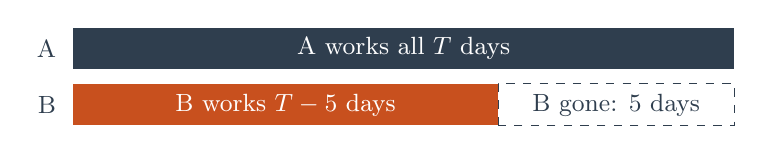
\begin{tikzpicture}[x=0.6cm,y=0.62cm,font=\small]
\fill[slate] (0,1.15) rectangle (14,2);
\fill[ember] (0,0) rectangle (9,0.85);
\draw[dashed,color=slate] (9,0) rectangle (14,0.85);
\node[anchor=east,color=slate] at (-0.15,1.57) {A};
\node[anchor=east,color=slate] at (-0.15,0.42) {B};
\node[color=white] at (7,1.57) {A works all $T$ days};
\node[color=white] at (4.5,0.42) {B works $T-5$ days};
\node[color=slate] at (11.5,0.42) {B gone: 5 days};
\end{tikzpicture}
\end{center}

\samp A takes 20 days and B takes 30 days. They work together, but B leaves 5 days before the work ends. What is the total time?
\begin{enumerate}
\item Total: LCM of 20 and 30 is 60 chairs.
\item A makes $60 \div 20 = 3$ chairs a day. B makes $60 \div 30 = 2$ chairs a day.
\item A works $T$ days and makes $3T$ chairs.
\item B works $T - 5$ days and makes $2(T - 5)$ chairs.
\item Together: $3T + 2(T - 5) = 60$.
\item So $5T - 10 = 60$, then $5T = 70$, then $T = 14$.
\item Check: A makes $14 \times 3 = 42$. B makes $9 \times 2 = 18$. And $42 + 18 = 60$.
\end{enumerate}
\ans{14 days.}

\samp A takes 12 days and B takes 6 days. A starts alone. B joins after 3 days. What is the total time?
\begin{enumerate}
\item Total: LCM of 12 and 6 is 12 chairs.
\item A makes $12 \div 12 = 1$ chair a day. B makes $12 \div 6 = 2$ chairs a day.
\item A works $T$ days and makes $T$ chairs.
\item B works $T - 3$ days and makes $2(T - 3)$ chairs.
\item Together: $T + 2(T - 3) = 12$.
\item So $3T - 6 = 12$, then $3T = 18$, then $T = 6$.
\item Check: A makes 6. B makes $3 \times 2 = 6$. And $6 + 6 = 12$.
\end{enumerate}
\ans{6 days.}

\tryit A takes 30 days and B takes 20 days. They work together, but B leaves 5 days before the work is finished. What is the total time?

\subsection{T8. Alternate days, in turns}
\spot ``A and B work on alternate days, A starting first.'' ``They work one day each, in turn.''

\mech
\begin{enumerate}
\item Find the total chairs and each person's chairs a day.
\item One cycle is 2 days: A's day, then B's day. Chairs in one cycle = A's chairs + B's chairs.
\item Count how many full cycles fit into the total. Note the chairs left over.
\item Finish the leftover day by day, in the same order. The last day may be only part of a day.
\item Total days = 2 $\times$ full cycles + the last days. \textbf{Who starts changes the answer.}
\end{enumerate}

\begin{center}
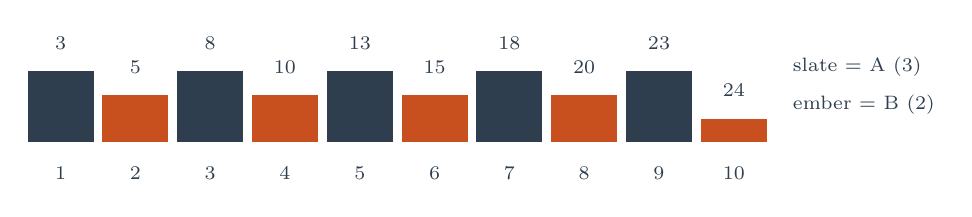
\begin{tikzpicture}[x=0.95cm,y=0.3cm,font=\scriptsize]
\foreach \dy/\qh/\qc/\qt in {1/3/slate/3,2/2/ember/5,3/3/slate/8,4/2/ember/10,5/3/slate/13,6/2/ember/15,7/3/slate/18,8/2/ember/20,9/3/slate/23,10/1/ember/24}{
  \fill[\qc] (\dy-1,0) rectangle (\dy-0.12,\qh);
  \node[color=slate] at (\dy-0.56,-1.3) {\dy};
  \node[color=slate] at (\dy-0.56,\qh+1.2) {\qt};
}
\node[anchor=west,color=slate] at (10.1,3.2) {slate = A (3)};
\node[anchor=west,color=slate] at (10.1,1.6) {ember = B (2)};
\end{tikzpicture}\par\nopagebreak\smallskip
{\small The sample below, day by day. The day number is under each bar and the running total of chairs is above it. On day 10, B needs only 1 more chair, which is half a day of B's work.}
\end{center}

\samp A takes 8 days and B takes 12 days. They work on alternate days. A starts. What is the total time?
\begin{enumerate}
\item Total: LCM of 8 and 12 is 24 chairs.
\item A makes $24 \div 8 = 3$ chairs a day. B makes $24 \div 12 = 2$ chairs a day.
\item One cycle of 2 days makes $3 + 2 = 5$ chairs.
\item 4 cycles (8 days) make 20 chairs. Chairs left: $24 - 20 = 4$.
\item Day 9 is A's day. A makes 3. Chairs left: 1.
\item Day 10 is B's day. B needs $1 \div 2 = \tfrac12$ day.
\item Total: $9 + \tfrac12 = 9.5$ days.
\end{enumerate}
\ans{9.5 days.}

\samp The same question, but B starts.
\begin{enumerate}
\item After 4 cycles (8 days), 20 chairs are made and 4 are left, as before.
\item Day 9 is B's day. B makes 2. Chairs left: 2.
\item Day 10 is A's day. A needs $2 \div 3 = \tfrac23$ day.
\item Total: $9 + \tfrac23 = 9\tfrac23$ days.
\end{enumerate}
\ans{$9\tfrac23$ days. A different starter gives a different answer.}

\samp A, B and C take 10, 15 and 30 days. They work one day each in the order A, B, C. What is the total time?
\begin{enumerate}
\item Total: LCM of 10, 15 and 30 is 30 chairs.
\item A makes 3, B makes 2 and C makes 1 chair a day.
\item One cycle of 3 days makes $3 + 2 + 1 = 6$ chairs.
\item $30 \div 6 = 5$ cycles, with nothing left over.
\item Total: $5 \times 3 = 15$ days.
\end{enumerate}
\ans{15 days.}

\tryit A takes 12 days and B takes 18 days. They work on alternate days. \textbf{B starts.} What is the total time?

\subsection{T9. Efficiency comparisons}
\spot ``A is twice as efficient as B.'' ``A is 25\% more efficient than B.'' ``A takes 60 days less than B.''

\mech
\begin{enumerate}
\item Efficiency means chairs a day.
\item Write the ratio of chairs a day from the sentence. The table shows the common ones.
\item Flip that ratio to get the ratio of days. The faster person takes fewer days.
\end{enumerate}

\begin{center}\small\renewcommand{\arraystretch}{1.18}\setlength{\tabcolsep}{9pt}
\begin{tabular}{@{}lll@{}}
\toprule
\textbf{\color{slate}The sentence} & \textbf{\color{slate}Chairs a day, A : B} & \textbf{\color{slate}Days, A : B} \\ \midrule
A is twice as efficient as B & 2 : 1 & 1 : 2 \\
A is three times as efficient as B & 3 : 1 & 1 : 3 \\
A is 25\% more efficient than B & 125 : 100 = 5 : 4 & 4 : 5 \\
B is 25\% less efficient than A & 100 : 75 = 4 : 3 & 3 : 4 \\
\bottomrule
\end{tabular}\end{center}

\samp A is twice as efficient as B. Together they finish a job in 12 days. How long does each take alone?
\begin{enumerate}
\item Chairs a day: A makes 2 and B makes 1.
\item Together they make $2 + 1 = 3$ chairs a day.
\item In 12 days they make $3 \times 12 = 36$ chairs. That is the whole job.
\item A alone: $36 \div 2 = 18$ days.
\item B alone: $36 \div 1 = 36$ days.
\end{enumerate}
\ans{A 18 days, B 36 days.}

\samp A is 25\% more efficient than B. B alone takes 20 days. How long does A take alone?
\begin{enumerate}
\item Chairs a day, A : B $= 5 : 4$.
\item Flip it. Days, A : B $= 4 : 5$.
\item B's 5 parts are 20 days, so 1 part is 4 days.
\item A's 4 parts are $4 \times 4 = 16$ days.
\end{enumerate}
\ans{16 days.}

\tryit A is 3 times as efficient as B. A alone takes 60 days less than B alone. How long do they take together?

\subsection{T10. Men, days and hours}
\spot ``12 men finish a job in 20 days working 6 hours a day.'' ``1 man works as much as 2 women.''

\mech
\begin{enumerate}
\item Count the work in \textbf{man-hours} = men $\times$ days $\times$ hours a day. If no hours are given, use man-days = men $\times$ days.
\item The same job always needs the same man-hours.
\item If the amount of work changes, first find the man-hours for one unit (one metre, one wall).
\item If there are two kinds of workers, change them all into one kind first.
\end{enumerate}
\textbf{As a formula.} $\dfrac{M_1 \times D_1 \times H_1}{W_1}=\dfrac{M_2 \times D_2 \times H_2}{W_2}$, where $M$ is men, $D$ is days, $H$ is hours a day and $W$ is the amount of work.

\samp 12 men finish a job in 20 days, working 6 hours a day. How many days will 15 men take, working 8 hours a day?
\begin{enumerate}
\item The job needs $12 \times 20 \times 6 = 1440$ man-hours.
\item The new team gives $15 \times 8 = 120$ man-hours a day.
\item Days: $1440 \div 120 = 12$.
\end{enumerate}
\ans{12 days.}

\samp 4 workers finish a job in 6 hours. How long will 3 workers take?
\begin{enumerate}
\item The job needs $4 \times 6 = 24$ worker-hours.
\item With 3 workers: $24 \div 3 = 8$ hours.
\end{enumerate}
\ans{8 hours.}

\samp 18 men build 270 m of road in 12 days. How many men are needed to build 450 m in 10 days?
\begin{enumerate}
\item 270 m needs $18 \times 12 = 216$ man-days.
\item One metre needs $216 \div 270 = 0.8$ man-days.
\item 450 m needs $450 \times 0.8 = 360$ man-days.
\item In 10 days: $360 \div 10 = 36$ men.
\end{enumerate}
\ans{36 men.}

\samp One man works as much as 2 women. 4 men and 4 women finish a job in 10 days. How long will 8 women take?
\begin{enumerate}
\item Change the men into women: 4 men are $4 \times 2 = 8$ women.
\item The team is $8 + 4 = 12$ women.
\item The job needs $12 \times 10 = 120$ woman-days.
\item With 8 women: $120 \div 8 = 15$ days.
\end{enumerate}
\ans{15 days.}

\sane More workers means fewer days. More work means more days. If your answer goes the other way, something is upside down.

\tryit 9 men lay 180 m of cable in 15 days, working 8 hours a day. How many days will 12 men take to lay 240 m, working 6 hours a day?

\subsection{T11. Part of the work}
\spot ``A completes $\tfrac35$ of the job in 12 days.'' ``40\% of the work in 8 days.'' ``A worked 6 days, then B finished the rest.''

\mech
\begin{enumerate}
\item Cut the job into equal parts (fifths, tenths).
\item Find the time for one part.
\item Multiply by the number of parts you need.
\item If someone else finishes the job, first find how many parts are left.
\end{enumerate}

\samp A completes $\tfrac35$ of a job in 12 days. How long does the whole job take?
\begin{enumerate}
\item 3 fifths take 12 days.
\item 1 fifth takes $12 \div 3 = 4$ days.
\item The whole job is 5 fifths: $5 \times 4 = 20$ days.
\end{enumerate}
\ans{20 days.}

\samp A does 40\% of a job in 8 days. How long does the whole job take?
\begin{enumerate}
\item 40\% takes 8 days.
\item 10\% takes $8 \div 4 = 2$ days.
\item 100\% takes $10 \times 2 = 20$ days.
\end{enumerate}
\ans{20 days.}

\samp A can do a job in 15 days. A works for 6 days. Then B finishes the rest in 6 days. How long would B take for the whole job alone?
\begin{enumerate}
\item A does 1 fifteenth a day. In 6 days A does 6 fifteenths, which is 2 fifths.
\item Left for B: $5 - 2 = 3$ fifths.
\item B does 3 fifths in 6 days, so 1 fifth in 2 days.
\item B does the whole job in $5 \times 2 = 10$ days.
\end{enumerate}
\ans{10 days.}

\tryit A can do a job in 20 days. A works alone for 8 days. Then B joins, and together they finish the rest in 6 more days. How long would B take alone?

\subsection{T12. Wages and sharing}
\spot ``They are paid Rs.\ 3000 for the job. Find each share.''

\mech
\begin{enumerate}
\item Money is shared by \textbf{chairs made}, not by days present.
\item Chairs made by a person = chairs a day $\times$ days that person actually worked.
\item A person's share = (their chairs $\div$ total chairs) $\times$ the money.
\item If everyone worked the same days, share in the ratio of chairs a day.
\end{enumerate}

\samp A can do a job in 10 days and B in 15 days. They do it together and are paid Rs.\ 3000. Find each share.
\begin{enumerate}
\item Total: LCM of 10 and 15 is 30 chairs.
\item A makes 3 chairs a day. B makes 2 chairs a day.
\item They work the same days, so share in the ratio $3 : 2$. That is 5 parts.
\item One part: $3000 \div 5 = 600$.
\item A gets $3 \times 600 = 1800$. B gets $2 \times 600 = 1200$.
\end{enumerate}
\ans{A Rs.\ 1800, B Rs.\ 1200.}

\samp The same A and B start together. A leaves after 3 days and B finishes the job. The pay is Rs.\ 3000. Find each share.
\begin{enumerate}
\item A works 3 days and makes $3 \times 3 = 9$ chairs.
\item B makes the other $30 - 9 = 21$ chairs.
\item Ratio $9 : 21 = 3 : 7$. That is 10 parts.
\item One part: $3000 \div 10 = 300$.
\item A gets $3 \times 300 = 900$. B gets $7 \times 300 = 2100$.
\end{enumerate}
\ans{A Rs.\ 900, B Rs.\ 2100.}

\tryit A, B and C can do a job alone in 10, 15 and 30 days. They do it together and are paid Rs.\ 6000. Find each share.

\subsection*{Shortcuts to memorise}
\begin{center}\small\renewcommand{\arraystretch}{1.75}\setlength{\tabcolsep}{8pt}
\begin{tabularx}{\linewidth}{@{}>{\raggedright\arraybackslash}X>{\raggedright\arraybackslash}X@{}}
\toprule
\textbf{\color{slate}Idea} & \textbf{\color{slate}Formula} \\ \midrule
Chairs a day & total chairs $\div$ days \\
Two people together & $\dfrac{x \times y}{x+y}$ days (two people only) \\
One person missing & $\dfrac{x \times T}{x-T}$ days ($x$ = known person alone, $T$ = team) \\
Three pairs given & add the three pairs' chairs a day, then halve \\
Men, days, hours & $\dfrac{M_1D_1H_1}{W_1}=\dfrac{M_2D_2H_2}{W_2}$ \\
Part of the work & find the time for one part, then multiply \\
Efficiency and days & the ratios are flipped \\
Wages & share by chairs a day $\times$ days actually worked \\
\bottomrule
\end{tabularx}\end{center}

\subsection*{Sanity checks before you mark the option}
\infobox{Ten seconds that save a wrong answer}{
\begin{itemize}
\item Working together is quicker than the quickest person alone.
\item A leak or an outlet makes filling slower. An extra inlet makes it faster.
\item More workers means fewer days. More work means more days.
\item Put the answer back. Do the chairs add up to the total?
\item Check the units: hours or minutes, days or hours a day.
\end{itemize}}

\subsection*{Traps}
\begin{enumerate}
\item \textbf{Adding days.} 10 days and 15 days do not make 25 days. Add chairs a day, never days.
\item \textbf{Using the two-person shortcut for three people.} It works for two only.
\item \textbf{Forgetting that a leak is a minus.}
\item \textbf{``After 3 days'' and ``3 days before the end'' are different.} After 3 days: you know the first part, so count chairs (T6). Before the end: you do not, so call the total $T$ (T7).
\item \textbf{Alternate days: ignoring who starts.} A first and B first give different answers (T8).
\item \textbf{Alternate days: dividing the total by the cycle and doubling.} That is wrong when chairs are left over. Finish the leftover day by day (T8).
\item \textbf{``25\% more'' and ``25\% less'' give different ratios.} A is 25\% more than B gives $5 : 4$. B is 25\% less than A gives $4 : 3$ (T9).
\item \textbf{Not flipping the ratio.} Chairs a day $2 : 1$ means days $1 : 2$ (T9).
\item \textbf{Sharing wages by days.} Share by chairs made (T12).
\item \textbf{Forgetting the hours a day} in man-hours questions (T10).
\end{enumerate}

\subsection*{Answers to ``Try it''}
\begin{center}\small\renewcommand{\arraystretch}{1.25}\setlength{\tabcolsep}{8pt}
\begin{tabularx}{\linewidth}{@{}l>{\raggedright\arraybackslash}p{3.4cm}>{\raggedright\arraybackslash}X@{}}
\toprule
\textbf{\color{slate}Type} & \textbf{\color{slate}Answer} & \textbf{\color{slate}Working, step by step} \\ \midrule
T1 & 12 days & Total 60 chairs. \newline A makes 3 a day, B makes 2 a day, together 5. \newline $60 \div 5 = 12$. \\
T2 & 12 days & Total 24 chairs. \newline Team 3 a day, A 1 a day, so B 2 a day. \newline $24 \div 2 = 12$. \\
T3 & 8 days & Total 60 chairs. \newline The pairs make 6, 4 and 5 a day. Sum 15. \newline Halve: 7.5 a day for all three. \newline $60 \div 7.5 = 8$. \\
T4 & 15 minutes & Total 60 litres. \newline A adds 3, B adds 2, C removes 1: net 4 a minute. \newline $60 \div 4 = 15$. \\
T5 & 20 hours & Total 20 litres. \newline Pipe 5 an hour, with the leak 4 an hour. \newline Leak 1 an hour. $20 \div 1 = 20$. \\
T6 & 10 more days (16 in all) & Total 60 chairs. A makes 3 a day, B makes 2. \newline 6 days together: $6 \times 5 = 30$ chairs. Left: 30. \newline A alone: $30 \div 3 = 10$. \\
T7 & 15 days & Total 60 chairs. A makes 2 a day, B makes 3. \newline $2T + 3(T - 5) = 60$. \newline $5T = 75$, so $T = 15$. \\
T8 & 14.5 days & Total 36 chairs. B makes 2 a day, A makes 3. \newline One cycle makes 5. 7 cycles (14 days) make 35. \newline 1 chair left. It is B's day: $\tfrac12$ day. \\
T9 & 22.5 days & Chairs a day $3 : 1$, so days $1 : 3$. \newline The gap of 2 parts is 60 days: A 30 days, B 90 days. \newline Total 90 chairs. A makes 3, B makes 1, together 4. \newline $90 \div 4 = 22.5$. \\
T10 & 20 days & 180 m needs $9 \times 15 \times 8 = 1080$ man-hours. \newline One metre needs 6. So 240 m needs 1440. \newline New team: $12 \times 6 = 72$ a day. $1440 \div 72 = 20$. \\
T11 & 20 days & Take 20 chairs. A makes 1 a day. \newline In 8 days A makes 8. Left: 12. \newline Together they make 12 in 6 days: 2 a day. \newline So B makes 1 a day: $20 \div 1 = 20$. \\
T12 & A Rs.\ 3000, B Rs.\ 2000, C Rs.\ 1000 & Chairs a day $3 : 2 : 1$, same days. \newline 6 parts, one part is 1000. \\
\bottomrule
\end{tabularx}\end{center}

\clearpage
\section[Speed, distance and time (S1--S12)]{Speed, distance and time (with trains, boats and races)}\label{ch:S}
\addtocontents{toc}{\protect\nopagebreak}

\subsection*{The one idea}
Distance = speed $\times$ time. Speed is a rate: kilometres covered in one hour, just as a work rate is chairs made in one day. Cover the thing you want in the triangle and read off the rest.

\begin{center}
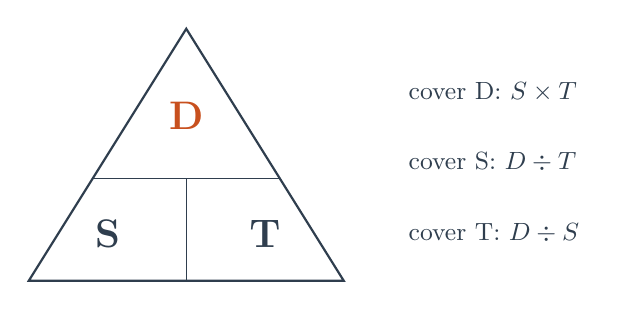
\begin{tikzpicture}[font=\small]
\draw[slate,thick] (0,0) -- (4,0) -- (2,3.2) -- cycle;
\draw[slate] (0.8125,1.3) -- (3.1875,1.3);
\draw[slate] (2,0) -- (2,1.3);
\node[font=\Large\bfseries,text=ember] at (2,2.1) {D};
\node[font=\Large\bfseries,text=slate] at (1,0.6) {S};
\node[font=\Large\bfseries,text=slate] at (3,0.6) {T};
\node[anchor=west,text=slate] at (4.7,2.4) {cover D: $S \times T$};
\node[anchor=west,text=slate] at (4.7,1.5) {cover S: $D \div T$};
\node[anchor=west,text=slate] at (4.7,0.6) {cover T: $D \div S$};
\end{tikzpicture}
\end{center}

\begin{center}\small\renewcommand{\arraystretch}{1.18}\setlength{\tabcolsep}{7pt}
\begin{tabularx}{\linewidth}{@{}l>{\raggedright\arraybackslash}X>{\raggedright\arraybackslash}X@{}}
\toprule
\textbf{\color{slate}If this is fixed} & \textbf{\color{slate}the other two} & \textbf{\color{slate}Example} \\ \midrule
Distance & are \textbf{opposite}: double the speed, half the time & 60 km at 30 km/h takes 2 h; at 60 km/h it takes 1 h \\
Time & move together: distance goes with speed & in 2 h, 30 km/h covers 60 km; 60 km/h covers 120 km \\
Speed & move together: distance goes with time & at 30 km/h, 2 h covers 60 km; 4 h covers 120 km \\
\bottomrule
\end{tabularx}\end{center}

\infobox{Two habits that remove most mistakes}{
\begin{enumerate}
\item \textbf{One unit system first.} Kilometres with hours, or metres with seconds. Never mix.
\item \textbf{No distance given? Make one up.} Take the LCM of the speeds, like the chairs in time and work. Every time becomes a whole number. Scale back at the end if the question gives a real time or distance (S3, S4).
\end{enumerate}}

\subsection*{Spot-it table}
Read the wording, find the row, jump to the type.
\begin{center}\small\renewcommand{\arraystretch}{1.18}\setlength{\tabcolsep}{7pt}
\begin{tabularx}{\linewidth}{@{}>{\raggedright\arraybackslash}X l >{\raggedright\arraybackslash}X@{}}
\toprule
\textbf{\color{slate}Wording in the question} & \textbf{\color{slate}Type} & \textbf{\color{slate}The one move} \\ \midrule
Covers... in..., change km/h to m/s & S1 & triangle, then convert units \\
Walks at $\tfrac34$ of usual speed, is late & S2 & speed and time are opposite \\
At 6 km/h late, at 8 km/h early & S3 & pick a distance, scale by the gap \\
Goes and returns, average speed & S4 & total distance $\div$ total time \\
Partly at $x$, partly at $y$, in $t$ hours & S5 & average, then split time by gaps \\
Towards each other, catches up, starts later & S6 & add or subtract the speeds \\
After meeting, they take 4 h and 9 h & S7 & speed ratio from square roots, flipped \\
Train crosses pole, platform, other train & S8 & right distance, right speed \\
Upstream, downstream, still water & S9 & still water = half the sum \\
Circular track, meet again & S10 & lap $\div$ sum or difference of speeds \\
Beats by 10 m, gives a start & S11 & same time, distances in speed ratio \\
Excluding and including stoppages & S12 & lost distance $\div$ running speed \\
\bottomrule
\end{tabularx}\end{center}

\subsection{S1. Basics and units}
\spot ``Covers 150 km in 2.5 hours. Speed?'' ``Change 72 km/h into m/s.'' ``Minutes to walk 800 m at 6 km/h?''

\mech
\begin{enumerate}
\item Put everything in one unit system: km with hours, or metres with seconds.
\item Distance = speed $\times$ time. Speed = distance $\div$ time. Time = distance $\div$ speed.
\item Change units with the table. Minutes to hours: divide by 60.
\end{enumerate}

\subsection{S2. Same distance: speed and time are opposite}
\spot ``Walking at $\tfrac56$ of his usual speed, he is 10 minutes late.'' ``Speed goes up by 25\%. By what percent does the time fall?''

\mech
\begin{enumerate}
\item The distance is the same, so the time ratio is the speed ratio \textbf{flipped}.
\item Write new : usual for the speeds. Flip it for the times.
\item The gap between the two times (in parts) is the delay. Find one part.
\item Usual time = its number of parts $\times$ one part.
\end{enumerate}

\samp Walking at $\tfrac56$ of his usual speed, he is 10 minutes late. What is his usual time?
\begin{enumerate}
\item Speeds, new : usual = 5 : 6.
\item Flip it. Times, new : usual = 6 : 5.
\item The gap is $6 - 5 = 1$ part. That part is the 10 minutes late.
\item Usual time = 5 parts = $5 \times 10 = 50$ minutes.
\item Check: the new time is 60 minutes, which is 10 more.
\end{enumerate}
\ans{50 minutes.}

\samp Speed goes up by 25\%. By what percent does the time fall?
\begin{enumerate}
\item Take the old speed as 100. The new speed is 125.
\item Times are flipped: new time = $\tfrac{100}{125} = \tfrac45$ of the old time.
\item The time falls by $\tfrac15$, which is 20\%.
\end{enumerate}
\ans{20\%.}

\textbf{Shortcuts.} Speed up by $x\%$: time falls by $\dfrac{x}{100+x}\times 100\%$. Speed down by $x\%$: time rises by $\dfrac{x}{100-x}\times 100\%$. (Speed down 20\% means time up 25\%.)

\tryit Walking at $\tfrac45$ of his usual speed, a student is 12 minutes late. What is his usual time?

\subsection{S3. Two speeds, early and late}
\spot ``At 6 km/h he is 10 minutes late. At 8 km/h he is 5 minutes early. Find the distance.''

\mech
\begin{enumerate}
\item Pick a pretend distance: the LCM of the two speeds.
\item Find the time at each speed. The gap between them is the \emph{pretend gap}.
\item Real gap = late minutes + early minutes. (Late at both, or early at both: subtract instead.)
\item Real distance = pretend distance $\times$ (real gap $\div$ pretend gap). Use hours for both gaps.
\end{enumerate}

\samp At 6 km/h he is 10 minutes late. At 8 km/h he is 5 minutes early. Find the distance.
\begin{enumerate}
\item Pretend distance: LCM of 6 and 8 is 24 km.
\item At 6 km/h: $24 \div 6 = 4$ hours. At 8 km/h: $24 \div 8 = 3$ hours.
\item Pretend gap: $4 - 3 = 1$ hour.
\item Real gap: $10 + 5 = 15$ minutes $= 0.25$ hour.
\item Real distance: $24 \times 0.25 \div 1 = 6$ km.
\item Check: 6 km takes 60 minutes at 6 km/h and 45 minutes at 8 km/h. On time is 50 minutes: 10 late, 5 early.
\end{enumerate}
\ans{6 km.}

\textbf{Shortcut.} Distance $=\dfrac{s_1 \times s_2}{s_2-s_1}\times$ gap in hours $=\dfrac{6\times 8}{2}\times 0.25=6$.

\tryit At 5 km/h he is 12 minutes late. At 6 km/h he is 3 minutes early. Find the distance.

\subsection{S4. Average speed}
\spot ``Goes at 40 km/h and returns at 60 km/h. Average speed?'' ``Half the way at ..., the rest at ...''

\mech
\begin{enumerate}
\item Average speed = \textbf{total distance $\div$ total time}.
\item Never just average the two speeds. (That works only when the \emph{times} are equal.)
\item No distance given? Pick one: the LCM of the speeds.
\end{enumerate}
\textbf{Shortcuts.} Equal distances at $x$ and $y$: average $=\dfrac{2xy}{x+y}$. Equal times at $x$ and $y$: average $=\dfrac{x+y}{2}$.

\samp He goes to town at 40 km/h and comes back at 60 km/h. Average speed?
\begin{enumerate}
\item Pick a distance: LCM of 40 and 60 is 120 km each way.
\item Going: $120 \div 40 = 3$ hours. Coming back: $120 \div 60 = 2$ hours.
\item Total distance: 240 km. Total time: 5 hours.
\item Average: $240 \div 5 = 48$ km/h.
\item Shortcut check: $\tfrac{2 \times 40 \times 60}{100} = 48$.
\end{enumerate}
\ans{48 km/h.}

\samp He drives 40 km/h for one hour, then 60 km/h for the next hour. Average speed?
\begin{enumerate}
\item Distance: $40 + 60 = 100$ km in 2 hours.
\item Average: $100 \div 2 = 50$ km/h. (Equal times, so the plain mean works.)
\end{enumerate}
\ans{50 km/h.}

\samp Half the journey at 30 km/h, half of the rest at 15 km/h, the remainder at 5 km/h. Average speed?
\begin{enumerate}
\item Pick 60 km. The parts are 30 km, 15 km and 15 km.
\item Times: $30 \div 30 = 1$ hour, $15 \div 15 = 1$ hour, $15 \div 5 = 3$ hours.
\item Total time: 5 hours.
\item Average: $60 \div 5 = 12$ km/h.
\end{enumerate}
\ans{12 km/h.}

\sane With equal distances the average is nearer the \emph{slower} speed (48 is nearer 40 than 60), because more time is spent going slowly.

\tryit (a) A cyclist goes to a town at 12 km/h and returns at 8 km/h. Average speed? (b) One third of a trip at 20 km/h, one third at 30 km/h and one third at 60 km/h. Average speed?

\subsection{S5. Two parts at two speeds, total given}
\spot ``100 km, partly at 20 km/h and the rest at 30 km/h, in 4 hours. How far at each speed?''

\mech
\begin{enumerate}
\item Average speed = total distance $\div$ total time.
\item Time at the slower speed : time at the faster speed = (faster $-$ average) : (average $-$ slower). (It is the mixtures trick.)
\item Split the total time in that ratio.
\item Distance for each part = speed $\times$ its time.
\end{enumerate}

\samp 100 km in 4 hours, partly at 20 km/h and partly at 30 km/h. How far at each speed?
\begin{enumerate}
\item Average: $100 \div 4 = 25$ km/h.
\item Time ratio, slower : faster = $(30 - 25) : (25 - 20) = 5 : 5 = 1 : 1$.
\item So 2 hours at each speed.
\item Distances: $20 \times 2 = 40$ km and $30 \times 2 = 60$ km.
\item Check: $40 \div 20 + 60 \div 30 = 2 + 2 = 4$ hours.
\end{enumerate}
\ans{40 km at 20 km/h, 60 km at 30 km/h.}

\sane The average must lie between the two speeds. 25 is between 20 and 30.

\tryit A man covers 180 km in 6 hours, partly at 25 km/h and the rest at 40 km/h. How far at each speed?

\subsection{S6. Relative speed: meeting and catching up}
\spot ``Two cars start 300 km apart and drive towards each other.'' ``B follows 2 hours later. When does B catch up?''

\mech
\begin{enumerate}
\item Moving towards each other (or apart): \textbf{add} the speeds.
\item Moving the same way: \textbf{subtract} the speeds.
\item Time = gap $\div$ that speed.
\item Head start: the gap = the first traveller's speed $\times$ the head-start time.
\end{enumerate}

\subsection{S7. Meet, then reach}
\spot ``After meeting, the first train takes 4 hours to reach the other's town and the second takes 9 hours. Ratio of speeds?''

\mech
\begin{enumerate}
\item Take the square root of each time after meeting.
\item Flip them: first's speed : second's speed $=\sqrt{\text{second's time}} : \sqrt{\text{first's time}}$.
\end{enumerate}
\emph{Why.} Before meeting both ran for the same time. After meeting, each must cover what the other covered. That makes the time ratio the square of the speed ratio, flipped.

\samp After meeting, the first train takes 4 hours and the second takes 9 hours. Ratio of their speeds?
\begin{enumerate}
\item Square roots: $\sqrt{4} = 2$ and $\sqrt{9} = 3$.
\item Flip them: first : second $= 3 : 2$.
\item Check with speeds 3 and 2. They meet after 6 hours, having covered 18 and 12.
\item The first then covers 12 at 3: 4 hours. The second covers 18 at 2: 9 hours. Both match.
\end{enumerate}
\ans{3 : 2.}

\tryit After meeting, the first train needs 9 hours and the second needs 16 hours. The first runs at 60 km/h. How fast is the second?

\subsection{S8. Trains}
\spot ``A 150 m train at 54 km/h crosses a pole, a 300 m platform, a man, another train.''

\mech
\begin{enumerate}
\item Change the speed to m/s when lengths are in metres.
\item Take the distance and the speed from the table.
\item Time = distance $\div$ speed.
\end{enumerate}

\subsection{S9. Boats and streams}
\spot Upstream, downstream, still water, current, stream.

\mech
\begin{enumerate}
\item Downstream speed $D$ = boat + stream. Upstream speed $U$ = boat $-$ stream.
\item Find $D$ and $U$ from distance $\div$ time for each leg.
\item Boat in still water $=\dfrac{D+U}{2}$. Stream $=\dfrac{D-U}{2}$.
\item ``Speed of the boat'' on its own means in still water.
\end{enumerate}

\samp A boat goes 30 km downstream in 2 hours and comes back the same 30 km in 3 hours. Find the boat's speed and the stream's speed.
\begin{enumerate}
\item Downstream: $D = 30 \div 2 = 15$ km/h.
\item Upstream: $U = 30 \div 3 = 10$ km/h.
\item Boat: $(15 + 10) \div 2 = 12.5$ km/h.
\item Stream: $(15 - 10) \div 2 = 2.5$ km/h.
\end{enumerate}
\ans{Boat 12.5 km/h, stream 2.5 km/h.}

\samp The boat's speed is 12 km/h and the stream's is 4 km/h. How long to go 48 km upstream and come back?
\begin{enumerate}
\item Downstream: $12 + 4 = 16$ km/h. Upstream: $12 - 4 = 8$ km/h.
\item Up: $48 \div 8 = 6$ hours. Down: $48 \div 16 = 3$ hours.
\item Total: $6 + 3 = 9$ hours.
\end{enumerate}
\ans{9 hours.}

\sane Upstream speed < still-water speed < downstream speed. A round trip on a stream always averages less than the still-water speed (here $96 \div 9 \approx 10.7$ km/h).

\tryit A boat goes 24 km upstream in 6 hours and 24 km downstream in 4 hours. Find the speed of the boat in still water and of the stream.

\subsection{S10. Circular track}
\spot ``Two runners start together on a 400 m circular track. When do they first meet?'' ``When are both back at the start?''

\mech
\begin{enumerate}
\item Opposite directions: first meeting after track length $\div$ (sum of the speeds).
\item Same direction: the faster must gain one full lap. Track length $\div$ (difference of the speeds).
\item Both back at the starting point together: LCM of their times for one lap.
\end{enumerate}

\samp A 400 m track. A runs at 5 m/s and B at 3 m/s. They start together. When do they first meet?
\begin{enumerate}
\item Opposite ways: $400 \div (5 + 3) = 50$ seconds.
\item Same way: $400 \div (5 - 3) = 200$ seconds.
\end{enumerate}
\ans{50 seconds opposite ways, 200 seconds the same way.}

\samp A takes 40 seconds a lap and B takes 60 seconds. They start together. When are both at the start together again?
\begin{enumerate}
\item LCM of 40 and 60 is 120.
\end{enumerate}
\ans{After 120 seconds.}

\tryit A 600 m track. A runs at 4 m/s and B at 6 m/s. They start together. When do they first meet if they run the same way? If they run opposite ways?

\subsection{S11. Races and head starts}
\spot ``A beats B by 10 m in a 100 m race.'' ``A gives B a 20 m start.'' ``A beats B by 5 seconds.''

\mech
\begin{enumerate}
\item ``A beats B by 10 m in 100 m'': when A has run 100 m, B has run 90 m.
\item They ran for the same time, so the speeds are in the same ratio: A : B $= 100 : 90 = 10 : 9$.
\item ``Beats by 5 seconds'': B needs 5 seconds more for the same race.
\item To compare A with C, multiply the ratios A : B and B : C.
\end{enumerate}

\samp In a 1000 m race A beats B by 100 m, and B beats C by 100 m. By how much does A beat C?
\begin{enumerate}
\item A : B $= 1000 : 900 = 10 : 9$.
\item B : C $= 1000 : 900 = 10 : 9$.
\item Multiply: A : C $= 100 : 81$.
\item While A runs 1000 m, C runs 810 m.
\end{enumerate}
\ans{By 190 m (not 200 m).}

\samp In a 100 m race A beats B by 20 m, or by 4 seconds. What is A's time?
\begin{enumerate}
\item B runs those last 20 m in 4 seconds, so B's speed is $20 \div 4 = 5$ m/s.
\item B's time for 100 m: $100 \div 5 = 20$ seconds.
\item A finishes 4 seconds earlier: $20 - 4 = 16$ seconds.
\item Check: in 16 seconds B runs 80 m, which is 20 m behind.
\end{enumerate}
\ans{16 seconds.}

\tryit A runs 100 m in 20 seconds and B runs it in 25 seconds. By how many metres does A beat B?

\subsection{S12. Stoppages}
\spot ``Without stoppages a bus runs at 60 km/h. With stoppages it averages 45 km/h. How many minutes does it stop each hour?''

\mech
\begin{enumerate}
\item In one hour, stops included, the bus covers the ``with stoppages'' distance.
\item At its running speed, that distance takes less than an hour.
\item The rest of the hour it is stopped.
\end{enumerate}
\textbf{Formula.} Stoppage per hour $=\dfrac{\text{without}-\text{with}}{\text{without}}\times 60$ minutes.

\samp Without stoppages 60 km/h, with stoppages 45 km/h. How long does it stop each hour?
\begin{enumerate}
\item In one hour the bus covers 45 km.
\item At 60 km/h, 45 km takes 45 minutes of running.
\item Stopped: $60 - 45 = 15$ minutes.
\item Formula check: $\tfrac{60 - 45}{60} \times 60 = 15$.
\end{enumerate}
\ans{15 minutes.}

\tryit Without stoppages a train runs at 72 km/h. With stoppages it averages 60 km/h. How many minutes does it stop each hour?

\subsection*{Shortcuts to memorise}
\begin{center}\small\renewcommand{\arraystretch}{1.75}\setlength{\tabcolsep}{8pt}
\begin{tabularx}{\linewidth}{@{}>{\raggedright\arraybackslash}X>{\raggedright\arraybackslash}X@{}}
\toprule
\textbf{\color{slate}Idea} & \textbf{\color{slate}Formula} \\ \midrule
Units & km/h $\times\tfrac{5}{18}$ = m/s; m/s $\times\tfrac{18}{5}$ = km/h \\
Same distance & speed ratio and time ratio are flips of each other \\
Speed up by $x\%$ & time falls by $\dfrac{x}{100+x}\times 100\%$ \\
Early and late & $D=\dfrac{s_1 s_2}{s_2-s_1}\times$ gap in hours \\
Average, equal distances & $\dfrac{2xy}{x+y}$ \\[6pt]
Average, equal times & $\dfrac{x+y}{2}$ \\[6pt]
Towards each other, same way & sum of speeds, difference of speeds \\
Meet, then reach & first : second $=\sqrt{t_2} : \sqrt{t_1}$ \\
Train and platform & train + platform length, at the train's speed \\
Boat and stream & still water $\dfrac{D+U}{2}$, stream $\dfrac{D-U}{2}$ \\
Circular track & length $\div$ sum (opposite) or $\div$ difference (same way) \\
Stoppage per hour & $\dfrac{\text{excl}-\text{incl}}{\text{excl}}\times 60$ minutes \\
\bottomrule
\end{tabularx}\end{center}

\subsection*{Sanity checks before you mark the option}
\infobox{Ten seconds that save a wrong answer}{
\begin{itemize}
\item Average speed lies between the two speeds, and nearer the slower one when distances are equal.
\item Closing speed (towards each other) is bigger than either speed. Catching-up speed is smaller.
\item Upstream speed is below still water, which is below downstream speed.
\item Same units on both sides: km with hours, metres with seconds.
\item Put the answer back: is distance = speed $\times$ time?
\end{itemize}}

\subsection*{Traps}
\begin{enumerate}
\item \textbf{Averaging the speeds.} For equal distances, $(40+60)\div 2 = 50$ is wrong. The answer is 48.
\item \textbf{Mixed units.} km/h with metres, or minutes with hours. Convert first.
\item \textbf{Early and late (S3).} Late at one speed and early at the other: add. Late at both (or early at both): subtract.
\item \textbf{Train and platform.} Forgetting the train's own length. The distance is train + platform.
\item \textbf{Adding when you should subtract.} Same direction subtracts, opposite adds. Draw the two arrows first.
\item \textbf{Head start.} The gap is speed $\times$ head-start time, not just the speed.
\item \textbf{Meeting point from the wrong town.} Distance from a town = that town's car's speed $\times$ time.
\item \textbf{Stream used once.} Downstream adds the stream, upstream subtracts it. ``Boat speed'' on its own means still water.
\item \textbf{Race margins.} ``Beats by 10 m in 100 m'' gives 100 : 90, not 100 : 10. Margins do not add: 100 m and 100 m in a 1000 m race gives 190 m, not 200 m.
\item \textbf{The delay in S2.} It is the \emph{difference} of the two times, which is one part, not the sum.
\end{enumerate}

\subsection*{Answers to ``Try it''}
\begin{center}\small\renewcommand{\arraystretch}{1.25}\setlength{\tabcolsep}{8pt}
\begin{tabularx}{\linewidth}{@{}l>{\raggedright\arraybackslash}p{3.4cm}>{\raggedright\arraybackslash}X@{}}
\toprule
\textbf{\color{slate}Type} & \textbf{\color{slate}Answer} & \textbf{\color{slate}Working, step by step} \\ \midrule
S1 & 200 m & 90 km/h $= 25$ m/s. \newline $25 \times 8 = 200$. \\
S2 & 48 minutes & Speeds 4 : 5, so times 5 : 4. \newline The gap of 1 part is 12 minutes. \newline Usual time = 4 parts = 48. \\
S3 & 7.5 km & Pretend distance 30 km: 6 hours and 5 hours, gap 1 hour. \newline Real gap 15 minutes $= 0.25$ hour. \newline $30 \times 0.25 = 7.5$. \\
S4 & (a) 9.6 km/h \newline (b) 30 km/h & (a) $2 \times 12 \times 8 \div 20 = 9.6$. \newline (b) Take 60 km each third. Times 3, 2 and 1 hours, total 6. $180 \div 6 = 30$. \\
S5 & 100 km at 25 km/h, 80 km at 40 km/h & Average $180 \div 6 = 30$. \newline Time ratio $(40 - 30) : (30 - 25) = 2 : 1$. \newline So 4 hours and 2 hours. \\
S6 & After 3 hours, 210 km & $70 + 80 = 150$ km/h. $450 \div 150 = 3$. \newline $70 \times 3 = 210$. \\
S7 & 45 km/h & First : second $= \sqrt{16} : \sqrt{9} = 4 : 3$. \newline $60 \times \tfrac34 = 45$. \\
S8 & 8 seconds & Same way: $72 - 18 = 54$ km/h $= 15$ m/s. \newline $120 \div 15 = 8$. \\
S9 & Boat 5 km/h, stream 1 km/h & $U = 24 \div 6 = 4$, $D = 24 \div 4 = 6$. \newline Boat $(6 + 4) \div 2 = 5$. Stream $(6 - 4) \div 2 = 1$. \\
S10 & 300 s same way, 60 s opposite ways & $600 \div (6 - 4) = 300$. \newline $600 \div (6 + 4) = 60$. \\
S11 & 20 m & A takes 20 seconds. B runs 4 m a second. \newline In 20 seconds B runs 80 m. \\
S12 & 10 minutes & $(72 - 60) \div 72 \times 60 = 10$. \\
\bottomrule
\end{tabularx}\end{center}

\clearpage
\section[Percentages (P1--P12)]{Percentages (with changes, votes and marks)}\label{ch:P}
\addtocontents{toc}{\protect\nopagebreak}

\subsection*{The one idea}
Percent means ``out of 100''. 35\% is $\tfrac{35}{100}$, and ``of'' means multiply, so 35\% of 240 is $\tfrac{35}{100}\times 240 = 84$. Every percent question asks for one of three things: the part, the percent, or the whole.

\begin{center}\small\renewcommand{\arraystretch}{1.18}\setlength{\tabcolsep}{9pt}
\begin{tabular}{@{}lll@{}}
\toprule
\textbf{\color{slate}You want} & \textbf{\color{slate}Do this} & \textbf{\color{slate}With 35\% of 240 = 84} \\ \midrule
The part & percent $\times$ whole $\div$ 100 & $35 \times 240 \div 100 = 84$ \\
The percent & part $\div$ whole $\times$ 100 & $84 \div 240 \times 100 = 35\%$ \\
The whole & part $\div$ percent $\times$ 100 & $84 \div 35 \times 100 = 240$ \\
\bottomrule
\end{tabular}\end{center}

\infobox{Two habits that remove most mistakes}{
\begin{enumerate}
\item \textbf{Percent of what?} The base is the number after ``of'', ``than'' or ``from''. For a change, it is the \emph{original} value.
\item \textbf{No number given? Start from 100.} It is the percent version of the chairs: every percent becomes that many units, and each change is easy to follow (P3, P6, P7).
\end{enumerate}}

\subsection*{Spot-it table}
Read the wording, find the row, jump to the type.
\begin{center}\small\renewcommand{\arraystretch}{1.18}\setlength{\tabcolsep}{7pt}
\begin{tabularx}{\linewidth}{@{}>{\raggedright\arraybackslash}X l >{\raggedright\arraybackslash}X@{}}
\toprule
\textbf{\color{slate}Wording in the question} & \textbf{\color{slate}Type} & \textbf{\color{slate}The one move} \\ \midrule
35\% of 240, 45 is what percent of 60 & P1 & part, percent or whole \\
Rises from 40 to 50, percent increase & P2 & change $\div$ original \\
Raised 20\% then cut 10\%, successive discounts & P3 & start from 100, apply in turn \\
After a 20\% rise it is 7200, original? & P4 & divide by the multiplier \\
Price up, cut use to spend the same & P5 & opposite: $\frac{r}{100+r}$ \\
A is 25\% more than B, B is what \% less? & P6 & put B at 100 \\
Length up 20\%, breadth down 10\%, area? & P7 & multiply the multipliers \\
Grows 10\% a year for 2 years & P8 & multiply once per year \\
Spends 40\% on rent, 25\% of the rest on food & P9 & percent of what is left \\
20\% votes invalid, winner got 55\% & P10 & valid votes first \\
Scores 40\%, fails by 30 marks & P11 & marks gap = percent gap \\
20\% of A = 30\% of B, A is 40\% of B & P12 & swap, ratio, or chain \\
\bottomrule
\end{tabularx}\end{center}

\subsection{P1. Basics and the fraction table}
\spot ``What is 35\% of 240?'' ``45 is what percent of 60?'' ``Write $\tfrac38$ as a percent.''

\mech
\begin{enumerate}
\item Part = percent $\times$ whole $\div$ 100.
\item Percent = part $\div$ whole $\times$ 100.
\item If the percent is in the table, use the fraction instead. It is faster.
\end{enumerate}

\subsection{P2. Percent change: increase and decrease}
\spot ``The price rises from 40 to 50. Percent increase?'' ``A salary of 24000 goes up by 12.5\%. New salary?''

\mech
\begin{enumerate}
\item Change = new $-$ old.
\item Percent change = change $\div$ \textbf{old} $\times$ 100. Always divide by the starting value.
\item To apply a change, multiply. Up $p\%$: multiply by $1 + \tfrac{p}{100}$. Down $p\%$: multiply by $1 - \tfrac{p}{100}$.
\end{enumerate}

\subsection{P3. Successive changes}
\spot ``Raised by 20\%, then cut by 10\%. Net change?'' ``Two discounts of 20\% and 25\%. One equal discount?''

\mech
\begin{enumerate}
\item Start from 100.
\item Apply each change in turn, on the new value each time.
\item Net percent = final value $-$ 100.
\end{enumerate}
\textbf{Formula.} With up as $+$ and down as $-$: net $= a + b + \dfrac{a \times b}{100}$.

\subsection{P4. Find the original}
\spot ``After a 20\% rise the salary is 7200. What was it before?'' ``After a 15\% discount the price is 850. Marked price?''

\mech
\begin{enumerate}
\item Take the original as 100 parts.
\item After the change it is (100 + rise) or (100 $-$ fall) parts.
\item The given new value is that many parts. Find one part.
\item Original = 100 parts.
\end{enumerate}
\textbf{Same thing in one line.} Original = new value $\div$ multiplier.

\samp After a 20\% rise the salary is 7200. What was it before?
\begin{enumerate}
\item Original: 100 parts. After the rise: 120 parts.
\item 120 parts = 7200, so 1 part = $7200 \div 120 = 60$.
\item Original: $100 \times 60 = 6000$.
\end{enumerate}
\ans{6000.}

\samp After a 15\% discount the price is 850. What was the marked price?
\begin{enumerate}
\item Marked price: 100 parts. After the discount: 85 parts.
\item 85 parts = 850, so 1 part = 10.
\item Marked price: $100 \times 10 = 1000$.
\end{enumerate}
\ans{1000.}

\samp A price goes up 10\%, then down 10\%, and ends at 990. What was it at first?
\begin{enumerate}
\item From 100: up 10\% gives 110. Down 10\% of 110 gives 99.
\item 99 parts = 990, so 1 part = 10.
\item Original: $100 \times 10 = 1000$.
\end{enumerate}
\ans{1000.}

\sane Do not take 20\% off 7200 to undo a 20\% rise. That gives 5760, which is wrong: the 20\% was of the \emph{old} value.

\tryit A shirt sells for 1360 after a 15\% discount. What was the marked price?

\subsection{P5. Price up, use down (spending stays the same)}
\spot ``Sugar costs 25\% more. By what percent must a family cut its use to spend the same?''

\mech
\begin{enumerate}
\item Spending = price $\times$ quantity.
\item Take the old price 100 and the old quantity 1. Spending is 100.
\item New quantity = 100 $\div$ new price.
\item Compare the new quantity with 1.
\end{enumerate}
\textbf{Shortcuts.} Price up $r\%$: use falls by $\dfrac{r}{100+r}\times 100\%$. Price down $r\%$: use can rise by $\dfrac{r}{100-r}\times 100\%$.

\samp The price goes up 25\%. By what percent must use fall?
\begin{enumerate}
\item New price: 125.
\item New quantity: $100 \div 125 = 0.8$.
\item From 1 to 0.8 is a fall of 0.2, which is 20\%.
\item Shortcut check: $25 \div 125 = 20\%$.
\end{enumerate}
\ans{20\%.}

\samp The price goes down 20\%. By what percent can use rise?
\begin{enumerate}
\item Shortcut: $20 \div (100 - 20) = 20 \div 80 = 25\%$.
\end{enumerate}
\ans{25\%.}

\samp The price goes up 20\% and the family cuts use by 10\%. What happens to spending?
\begin{enumerate}
\item New spending $= 1.2 \times 0.9 = 1.08$ of the old.
\end{enumerate}
\ans{Spending goes up 8\%.}

\tryit (a) The price goes up 50\%. By what percent must use fall to spend the same? (b) The price falls by $16\tfrac23\%$. By what percent can use rise?

\subsection{P6. More than, less than}
\spot ``A's salary is 25\% more than B's. B's salary is what percent less than A's?''

\mech
\begin{enumerate}
\item Put the person after ``than'' at 100.
\item Work out the other person.
\item Now answer the new question. Divide the gap by the \emph{new} person after ``than''.
\end{enumerate}
\textbf{Shortcuts.} A is $x\%$ more than B: B is $\dfrac{x}{100+x}\times 100\%$ less than A. A is $x\%$ less than B: B is $\dfrac{x}{100-x}\times 100\%$ more than A.

\samp A is 25\% more than B. B is what percent less than A?
\begin{enumerate}
\item B = 100, so A = 125.
\item The gap is 25. Now it is ``less than A'', so divide by A.
\item $25 \div 125 = 20\%$.
\end{enumerate}
\ans{20\%.}

\samp A is 20\% less than B. B is what percent more than A?
\begin{enumerate}
\item B = 100, so A = 80.
\item The gap is 20. Now it is ``more than A'', so divide by A.
\item $20 \div 80 = 25\%$.
\end{enumerate}
\ans{25\%.}

\tryit Ravi earns 60\% more than Mohan. Mohan earns what percent less than Ravi?

\subsection{P7. Two changes multiplied: area and products}
\spot ``Length up 20\%, breadth down 10\%. Change in area?'' ``The side of a square goes up 10\%. Change in area?''

\mech
\begin{enumerate}
\item Area = length $\times$ breadth. So multiply the two multipliers.
\item A square or a circle has the same change twice, so square the multiplier.
\item Compare the result with 1.
\end{enumerate}
\textbf{Shortcut.} Side or radius up $x\%$: area up $\left(2x + \tfrac{x^2}{100}\right)\%$.

\samp A rectangle's length goes up 20\% and its breadth goes down 10\%. Change in area?
\begin{enumerate}
\item Multipliers: 1.2 and 0.9.
\item $1.2 \times 0.9 = 1.08$.
\end{enumerate}
\ans{Area up 8\%.}

\samp A square's side goes up 10\%. A circle's radius goes down 20\%. Change in each area?
\begin{enumerate}
\item Square: $1.1 \times 1.1 = 1.21$, so up 21\% (not 10\%).
\item Circle: $0.8 \times 0.8 = 0.64$, so down 36\%.
\end{enumerate}
\ans{Square up 21\%, circle down 36\%.}

\tryit (a) Length up 30\%, breadth down 10\%. Change in area? (b) A circle's radius goes up 50\%. Change in area?

\subsection{P8. Repeated change: population and depreciation}
\spot ``A town of 20000 grows 10\% a year. After 2 years?'' ``A machine loses 10\% of its value every year.''

\mech
\begin{enumerate}
\item Multiply by the multiplier once for every year.
\item Growth: $1 + \tfrac{r}{100}$. Fall: $1 - \tfrac{r}{100}$.
\item Different rates in different years: multiply each year's own multiplier.
\item To go back in time, divide instead.
\end{enumerate}

\samp A population of 20000 grows 10\% a year. What is it after 2 years?
\begin{enumerate}
\item Year 1: $20000 \times 1.1 = 22000$.
\item Year 2: $22000 \times 1.1 = 24200$.
\end{enumerate}
\ans{24200.}

\samp A machine worth 80000 loses 10\% of its value each year. Value after 2 years?
\begin{enumerate}
\item Year 1: $80000 \times 0.9 = 72000$.
\item Year 2: $72000 \times 0.9 = 64800$.
\end{enumerate}
\ans{64800.}

\samp A population of 50000 grows 20\% in the first year and 10\% in the second. What is it then?
\begin{enumerate}
\item Year 1: $50000 \times 1.2 = 60000$.
\item Year 2: $60000 \times 1.1 = 66000$.
\end{enumerate}
\ans{66000.}

\sane Two years at 10\% is 21\%, not 20\%. The second year's 10\% is on a bigger number.

\tryit A village has 26620 people now, after growing 10\% a year for 3 years. How many were there 3 years ago?

\subsection{P9. Spending split: percent of what is left}
\spot ``Spends 40\% on rent, 25\% of the rest on food, and saves the remaining 4500. Salary?''

\mech
\begin{enumerate}
\item Take the salary as 100\%.
\item After each item, write what is left.
\item ``25\% of the rest'' means 25\% of what is left, not of the salary.
\item The last amount left equals the money given. Find the salary.
\end{enumerate}

\samp He spends 40\% on rent, 25\% of the rest on food, and saves 4500. What is his salary?
\begin{enumerate}
\item After rent: $100\% - 40\% = 60\%$ left.
\item Food: 25\% of 60\% is 15\% of the salary.
\item After food: $60\% - 15\% = 45\%$ left.
\item 45\% of the salary = 4500. So 1\% = 100.
\item Salary: $100 \times 100 = 10000$.
\end{enumerate}
\ans{10000.}

\samp A man spends 75\% of his income and saves the rest. His income rises 20\% and his spending rises 10\%. What happens to his savings?
\begin{enumerate}
\item Old: income 100, spending 75, savings 25.
\item New income: 120. New spending: $75 \times 1.1 = 82.5$.
\item New savings: $120 - 82.5 = 37.5$.
\item Savings rose by 12.5 on 25, which is 50\%.
\end{enumerate}
\ans{Savings rise 50\%.}

\tryit A man spends 20\% of his salary on rent, 30\% of the rest on food, and has 5600 left. What is his salary?

\subsection{P10. Votes and elections}
\spot ``20\% of the votes were invalid. The winner got 55\% of the valid votes and won by 2400. How many votes were cast?''

\mech
\begin{enumerate}
\item The candidates' percents are of the \emph{valid} votes.
\item Margin percent = winner's percent $-$ loser's percent.
\item Margin votes = margin percent of the valid votes. Find the valid votes.
\item Valid votes are (100 $-$ invalid)\% of all votes. Find all the votes.
\end{enumerate}

\samp 20\% of votes were invalid. The winner got 55\% of the valid votes and won by 2400 votes. How many votes were cast?
\begin{enumerate}
\item The loser got $100 - 55 = 45\%$ of the valid votes.
\item Margin: $55 - 45 = 10\%$ of the valid votes = 2400.
\item Valid votes: $2400 \times 10 = 24000$.
\item Valid votes are 80\% of all votes. All votes: $24000 \div 0.8 = 30000$.
\item Check: the winner got 13200, the loser 10800. The difference is 2400.
\end{enumerate}
\ans{30000 votes.}

\tryit In a two-candidate election 10\% of the votes are invalid. The winner gets 60\% of the valid votes and wins by 3600 votes. How many votes were cast?

\subsection{P11. Marks and passing}
\spot ``One student scores 40\% and fails by 30 marks. Another scores 50\% and passes by 20 marks. Maximum marks?''

\mech
\begin{enumerate}
\item Both students are measured against the same pass mark.
\item Marks gap between them = fails by + passes by. (Both fail, or both pass: subtract.)
\item Percent gap = the difference of their percents.
\item Marks gap is that percent of the maximum. Find the maximum.
\item Pass mark = first student's marks + the marks he was short.
\end{enumerate}

\samp One student scores 40\% and fails by 30 marks. Another scores 50\% and passes by 20 marks. Find the maximum marks and the pass mark.
\begin{enumerate}
\item Marks gap: $30 + 20 = 50$.
\item Percent gap: $50\% - 40\% = 10\%$.
\item 10\% of the maximum = 50, so the maximum is 500.
\item First student: 40\% of 500 = 200. Pass mark: $200 + 30 = 230$.
\item Check: the second student has 50\% of 500 = 250, which is $230 + 20$.
\end{enumerate}
\ans{Maximum 500, pass mark 230.}

\tryit One student scores 30\% and fails by 15 marks. Another scores 40\% and passes by 25 marks. Find the maximum marks and the pass mark.

\subsection{P12. \texorpdfstring{$x\%$ of $y$}{x percent of y}, ratios and chains}
\spot ``Find 72\% of 25.'' ``20\% of A equals 30\% of B. Find A : B.'' ``A is 40\% of B and B is 50\% of C.''

\mech
\begin{enumerate}
\item $x\%$ of $y$ is the same as $y\%$ of $x$. Swap to the easier one.
\item $x\%$ of A $= y\%$ of B gives A : B $= y : x$. (Swap the percents.)
\item A is $x\%$ of B and B is $y\%$ of C: A is $\tfrac{x \times y}{100}\%$ of C.
\end{enumerate}

\samp Find 72\% of 25.
\begin{enumerate}
\item Swap: 72\% of 25 = 25\% of 72.
\item 25\% is a quarter: $72 \div 4 = 18$.
\end{enumerate}
\ans{18.}

\samp 20\% of A equals 30\% of B. Find A : B.
\begin{enumerate}
\item Swap the percents: A : B $= 30 : 20 = 3 : 2$.
\item Check with A = 3 and B = 2: $0.2 \times 3 = 0.6$ and $0.3 \times 2 = 0.6$.
\end{enumerate}
\ans{3 : 2.}

\samp A is 40\% of B, and B is 50\% of C. A is what percent of C?
\begin{enumerate}
\item $40 \times 50 \div 100 = 20$.
\end{enumerate}
\ans{20\%.}

\tryit (a) Find 8\% of 75. (b) 25\% of A equals 40\% of B. Find A : B.

\subsection*{Shortcuts to memorise}
\begin{center}\small\renewcommand{\arraystretch}{1.9}\setlength{\tabcolsep}{8pt}
\begin{tabularx}{\linewidth}{@{}>{\raggedright\arraybackslash}X>{\raggedright\arraybackslash}X@{}}
\toprule
\textbf{\color{slate}Idea} & \textbf{\color{slate}Formula} \\ \midrule
Part, percent, whole & percent $\times$ whole $\div$ 100;\quad part $\div$ whole $\times$ 100 \\
Percent change & $\dfrac{\text{new}-\text{old}}{\text{old}}\times 100$ \\
Two changes $a\%$ and $b\%$ & net $=a+b+\dfrac{ab}{100}$ \\
Up $x\%$ then down $x\%$ & $-\dfrac{x^2}{100}\%$ \\
Original & new $\div$ multiplier \\
Price up $r\%$, spending fixed & quantity down $\dfrac{r}{100+r}\times 100\%$ \\
A is $x\%$ more than B & B is $\dfrac{x}{100+x}\times 100\%$ less than A \\
Side up $x\%$ & area up $\left(2x+\dfrac{x^2}{100}\right)\%$ \\
Growth over $n$ years & $P\left(1+\dfrac{r}{100}\right)^n$ \\
$x\%$ of $y$ & equals $y\%$ of $x$ \\
\bottomrule
\end{tabularx}\end{center}

\subsection*{Sanity checks before you mark the option}
\infobox{Ten seconds that save a wrong answer}{
\begin{itemize}
\item A rise followed by an equal fall ends below the start.
\item ``25\% more'' and ``25\% less'' are not opposites: 25\% more is 20\% less the other way round.
\item A change is a percent of the old value. Vote shares are percents of the valid votes.
\item Put the answer back: start from 100 and apply the changes. Do you land on the given number?
\item Percent or percentage points? Read the question again.
\end{itemize}}

\subsection*{Traps}
\begin{enumerate}
\item \textbf{Dividing by the new value.} Percent change is out of the old value (P2).
\item \textbf{Adding successive percents.} 20\% then 10\% is 32\%, not 30\% (P3).
\item \textbf{Up then down is not zero.} 10\% up then 10\% down leaves you 1\% below (P3).
\item \textbf{Undoing a change from the new value.} Divide by the multiplier. Do not take the percent off the new value (P4).
\item \textbf{More than versus less than.} 25\% more than B means B is 20\% less than A, not 25\% (P6).
\item \textbf{Area changes by more than the side.} Side up 10\% means area up 21\%, not 10\% (P7).
\item \textbf{Two years at 10\% is 21\%.} Multiply the years, do not add them (P8).
\item \textbf{``Percent of the rest'' taken from the whole.} It is a percent of what is left (P9).
\item \textbf{Votes.} Shares are of the valid votes, but the question asks for total votes. Do not forget the last division (P10).
\item \textbf{Marks.} Fails by 30 and passes by 20 make a gap of 50, not 10 (P11).
\item \textbf{Percentage points versus percent.} 10\% to 12\% is 2 points, but a 20\% rise (P2).
\end{enumerate}

\subsection*{Answers to ``Try it''}
\begin{center}\small\renewcommand{\arraystretch}{1.25}\setlength{\tabcolsep}{8pt}
\begin{tabularx}{\linewidth}{@{}l>{\raggedright\arraybackslash}p{3.4cm}>{\raggedright\arraybackslash}X@{}}
\toprule
\textbf{\color{slate}Type} & \textbf{\color{slate}Answer} & \textbf{\color{slate}Working, step by step} \\ \midrule
P1 & (a) 200 \newline (b) 35\% & (a) $62\tfrac12\% = \tfrac58$. $320 \div 8 \times 5 = 200$. \newline (b) $28 \div 80 \times 100 = 35$. \\
P2 & (a) 20\% \newline (b) 25\% & (a) Change 50 on old 250: $50 \div 250$. \newline (b) Change 50 on old 200: $50 \div 200$. \\
P3 & (a) up 50\% \newline (b) down 4\% & (a) $100 \to 125 \to 150$. \newline (b) $100 \to 80 \to 96$. \\
P4 & 1600 & 85 parts = 1360, so 1 part = 16. \newline 100 parts = 1600. \\
P5 & (a) $33\tfrac13\%$ \newline (b) 20\% & (a) $50 \div 150$. \newline (b) $16\tfrac23\% = \tfrac16$. Price 6 becomes 5, so use 5 becomes 6: up $\tfrac15$. \\
P6 & 37.5\% & Mohan 100, Ravi 160. \newline Gap 60 on Ravi: $60 \div 160$. \\
P7 & (a) up 17\% \newline (b) up 125\% & (a) $1.3 \times 0.9 = 1.17$. \newline (b) $1.5 \times 1.5 = 2.25$. \\
P8 & 20000 & Divide by 1.1 three times: \newline $26620 \to 24200 \to 22000 \to 20000$. \\
P9 & 10000 & After rent 80\% left. Food: 30\% of 80\% = 24\%. \newline Left: 56\% = 5600. So 1\% = 100. \\
P10 & 20000 & Margin $60 - 40 = 20\%$ of valid = 3600. \newline Valid 18000. All votes: $18000 \div 0.9$. \\
P11 & Maximum 400, pass mark 135 & Marks gap $15 + 25 = 40$ = 10\% of maximum. \newline Maximum 400. Pass: 30\% of 400 + 15 = 135. \\
P12 & (a) 6 \newline (b) 8 : 5 & (a) 75\% of 8 $= 6$. \newline (b) Swap: $40 : 25 = 8 : 5$. \\
\bottomrule
\end{tabularx}\end{center}

\clearpage
\section[Ratio and proportion (R1--R12)]{Ratio and proportion (with sharing, ages and partnership)}\label{ch:R}
\addtocontents{toc}{\protect\nopagebreak}

\subsection*{The one idea}
A ratio compares quantities in \textbf{parts}. 3 : 2 means 3 parts and 2 parts, and every part is the same size. Almost every ratio question comes down to one step: \emph{find what one part is worth}, then multiply.

\begin{center}\small\renewcommand{\arraystretch}{1.18}\setlength{\tabcolsep}{9pt}
\begin{tabular}{@{}ll@{}}
\toprule
\textbf{\color{slate}What you are given} & \textbf{\color{slate}One part is} \\ \midrule
the total & total $\div$ sum of the ratio terms \\
the difference & difference $\div$ difference of the ratio terms \\
one share & that share $\div$ its ratio term \\
\bottomrule
\end{tabular}\end{center}

\infobox{Two habits that remove most mistakes}{
\begin{enumerate}
\item \textbf{Find one part first.} After that, every share is its ratio term times one part.
\item \textbf{Same unit, same order.} A ratio has no unit, so both terms must be in the same unit. A : B is not B : A.
\end{enumerate}}

\subsection*{Spot-it table}
Read the wording, find the row, jump to the type.
\begin{center}\small\renewcommand{\arraystretch}{1.18}\setlength{\tabcolsep}{7pt}
\begin{tabularx}{\linewidth}{@{}>{\raggedright\arraybackslash}X l >{\raggedright\arraybackslash}X@{}}
\toprule
\textbf{\color{slate}Wording in the question} & \textbf{\color{slate}Type} & \textbf{\color{slate}The one move} \\ \midrule
Simplify 48 : 72, which ratio is greater & R1 & HCF, cross-multiply \\
Divide 4500 in the ratio 2 : 3 : 4 & R2 & find one part \\
A : B = 2 : 3 and B : C = 4 : 5 & R3 & match the shared term (LCM) \\
Add 10 to each, ratio becomes 5 : 7; ages & R4 & the difference stays the same \\
24 women join, ratio becomes 1 : 2 & R5 & the unchanged term is the anchor \\
6 pens cost 90; 8 workers take 12 days & R6 & direct: one unit; inverse: product \\
Fourth, third, mean proportional & R7 & extremes product = means product \\
Compound, duplicate, sub-duplicate ratio & R8 & multiply, square, root \\
$\tfrac23$ of B, 25\% more, $\tfrac12 : \tfrac13 : \tfrac14$ & R9 & turn into whole-number terms \\
Rs.\ 1, 50 paise, 25 paise coins in a ratio & R10 & multiply by the worth of a coin \\
Two classes with different ratios, combined & R11 & real numbers first, then add \\
Invests 5000 for 12 months, 8000 for 6 & R12 & investment $\times$ time \\
\bottomrule
\end{tabularx}\end{center}

\subsection{R1. Basics: simplify, compare, units}
\spot ``Simplify 48 : 72.'' ``Ratio of 90 cm to 1.5 m.'' ``Which is greater, 3 : 4 or 5 : 7?''

\mech
\begin{enumerate}
\item Put both terms in the same unit first.
\item Simplify: divide both terms by their HCF.
\item To compare $a : b$ with $c : d$, cross-multiply. Compare $a \times d$ with $b \times c$. The bigger product goes with the bigger ratio.
\end{enumerate}

\samp Simplify 48 : 72.
\begin{enumerate}
\item HCF of 48 and 72 is 24.
\item $48 \div 24 = 2$ and $72 \div 24 = 3$.
\end{enumerate}
\ans{2 : 3.}

\samp Find the ratio of 90 cm to 1.5 m.
\begin{enumerate}
\item Same unit: 1.5 m = 150 cm.
\item $90 : 150$. Divide both by 30.
\end{enumerate}
\ans{3 : 5.}

\samp Which is greater, 3 : 4 or 5 : 7?
\begin{enumerate}
\item Cross-multiply: $3 \times 7 = 21$ and $4 \times 5 = 20$.
\item 21 is bigger, and it came from 3 : 4.
\item Check: $0.75 > 0.714$.
\end{enumerate}
\ans{3 : 4.}

\tryit (a) The ratio of 45 minutes to 2 hours. (b) Which is greater, 5 : 8 or 7 : 12?

\subsection{R2. Sharing in a ratio}
\spot ``Divide 4500 in the ratio 2 : 3 : 4.'' ``Two numbers are in the ratio 7 : 4 and differ by 600.''

\mech
\begin{enumerate}
\item Total given: one part = total $\div$ sum of the ratio terms.
\item Difference given: one part = difference $\div$ difference of the terms.
\item One share given: one part = that share $\div$ its term.
\item Each share = its term $\times$ one part.
\end{enumerate}

\subsection{R3. Joining two ratios}
\spot ``A : B = 2 : 3 and B : C = 4 : 5. Find A : B : C.''

\mech
\begin{enumerate}
\item Find the letter that is in both ratios (B).
\item Make B the same number in both: use the LCM of B's two numbers.
\item Scale each ratio to that number. Then write them side by side.
\end{enumerate}

\samp A : B = 2 : 3 and B : C = 4 : 5. Find A : B : C.
\begin{enumerate}
\item B is 3 in one ratio and 4 in the other. LCM of 3 and 4 is 12.
\item A : B $= 2 : 3$. Multiply by 4: $8 : 12$.
\item B : C $= 4 : 5$. Multiply by 3: $12 : 15$.
\item Join them: A : B : C $= 8 : 12 : 15$.
\end{enumerate}
\ans{8 : 12 : 15.}

\samp Now also C : D = 6 : 7. Find A : B : C : D.
\begin{enumerate}
\item C is 15 in A : B : C and 6 in C : D. LCM of 15 and 6 is 30.
\item A : B : C $= 8 : 12 : 15$. Multiply by 2: $16 : 24 : 30$.
\item C : D $= 6 : 7$. Multiply by 5: $30 : 35$.
\item Join them: $16 : 24 : 30 : 35$.
\end{enumerate}
\ans{16 : 24 : 30 : 35.}

\sane Shrink back: 8 : 12 is 2 : 3, and 12 : 15 is 4 : 5, as given.

\tryit A : B = 3 : 4 and B : C = 6 : 7. Find A : B : C.

\subsection{R4. The same number added to both}
\spot ``Two numbers are 3 : 5. Add 10 to each and they become 5 : 7.'' ``Ages are 5 : 4. Five years ago they were 4 : 3.''

\mech
\begin{enumerate}
\item Adding the same number to both keeps their \textbf{difference} the same.
\item So scale the two ratios until their differences (in parts) are equal.
\item Look at one number before and after. Its change in parts = the number added.
\item That gives one part. Multiply out.
\end{enumerate}

\subsection{R5. Only one quantity changes}
\spot ``Men and women are 3 : 5. After 24 women join, the ratio is 1 : 2.''

\mech
\begin{enumerate}
\item The quantity that did \emph{not} change is the anchor.
\item Scale the new ratio so the anchor has the same number of parts as before.
\item The other quantity's change in parts = the number added (or removed). Find one part.
\item Multiply out the old ratio.
\end{enumerate}

\samp Men : women $= 3 : 5$. After 24 women join, the ratio is $1 : 2$. How many of each were there?
\begin{enumerate}
\item The men did not change. They are the anchor: 3 parts.
\item Scale $1 : 2$ to $3 : 6$, so the men are 3 parts again.
\item Women went from 5 parts to 6 parts: 1 part = 24.
\item Men: $3 \times 24 = 72$. Women: $5 \times 24 = 120$.
\item Check: $72 : 144 = 1 : 2$.
\end{enumerate}
\ans{72 men, 120 women.}

\samp Boys : girls $= 5 : 7$. After 12 girls join, the ratio is $5 : 9$. How many of each were there?
\begin{enumerate}
\item Boys are the anchor, already 5 parts in both.
\item Girls went from 7 parts to 9 parts: 2 parts = 12, so 1 part = 6.
\item Boys: $5 \times 6 = 30$. Girls: $7 \times 6 = 42$.
\end{enumerate}
\ans{30 boys, 42 girls.}

\samp Red : blue marbles $= 4 : 3$. After 10 red marbles are taken out, the ratio is $2 : 3$. How many of each were there?
\begin{enumerate}
\item Blue is the anchor, 3 parts in both.
\item Red went from 4 parts to 2 parts: 2 parts = 10, so 1 part = 5.
\item Red: $4 \times 5 = 20$. Blue: $3 \times 5 = 15$.
\item Check: $10 : 15 = 2 : 3$.
\end{enumerate}
\ans{20 red, 15 blue.}

\sane Did both change by the same amount? Then it is R4, not R5.

\tryit Pens : pencils $= 2 : 3$. After 15 pencils are added, the ratio is $4 : 9$. How many pens and pencils were there at first?

\subsection{R6. Direct and inverse proportion}
\spot ``6 pens cost 90. What do 10 pens cost?'' ``8 workers take 12 days. How long will 6 workers take?''

\mech
\begin{enumerate}
\item Ask: if one doubles, what does the other do?
\item It doubles too: \textbf{direct}. Find the value of one unit, then multiply.
\item It halves: \textbf{inverse}. The product stays the same. Find the product, then divide.
\end{enumerate}

\subsection{R7. Proportion: fourth, third and mean proportional}
\spot ``Find $x$ if 3 : $x$ = 12 : 20.'' ``Fourth proportional to 4, 6, 10.'' ``Third proportional to 4 and 6.'' ``Mean proportional between 4 and 9.''

\mech
\begin{enumerate}
\item $a : b = c : d$ means $a \times d = b \times c$ (outer product = inner product).
\item Fourth proportional to $a, b, c$: $d = \dfrac{b \times c}{a}$.
\item Third proportional to $a$ and $b$: $c = \dfrac{b \times b}{a}$.
\item Mean proportional between $a$ and $b$: $\sqrt{a \times b}$.
\end{enumerate}

\samp Find $x$ if $3 : x = 12 : 20$.
\begin{enumerate}
\item Outer product = inner product: $3 \times 20 = 12 \times x$.
\item $60 = 12x$, so $x = 5$.
\end{enumerate}
\ans{5.}

\samp Find the fourth proportional to 4, 6, 10; the third proportional to 4 and 6; and the mean proportional between 4 and 9.
\begin{enumerate}
\item Fourth: $6 \times 10 \div 4 = 15$. Check: $4 : 6 = 10 : 15$.
\item Third: $6 \times 6 \div 4 = 9$. Check: $4 : 6 = 6 : 9$.
\item Mean: $\sqrt{4 \times 9} = \sqrt{36} = 6$.
\end{enumerate}
\ans{15, 9 and 6.}

\tryit (a) Find $x$ if $x : 18 = 14 : 21$. (b) Mean proportional between 12 and 27. (c) Third proportional to 9 and 12.

\subsection{R8. Compound, duplicate and sub-duplicate ratios}
\spot ``Compound ratio of 2 : 3 and 4 : 5.'' ``Duplicate ratio of 3 : 4.'' ``Sub-duplicate ratio of 9 : 16.''

\mech
\begin{enumerate}
\item Compound ratio of $a : b$ and $c : d$: multiply straight across, $a \times c : b \times d$.
\item Duplicate: square both terms. Triplicate: cube both terms.
\item Sub-duplicate: square root of both terms. Sub-triplicate: cube root.
\end{enumerate}

\samp Find the compound ratio of 2 : 3 and 4 : 5, the duplicate of 3 : 4, the triplicate of 2 : 3 and the sub-duplicate of 9 : 16.
\begin{enumerate}
\item Compound: $2 \times 4 : 3 \times 5 = 8 : 15$.
\item Duplicate of 3 : 4: $9 : 16$.
\item Triplicate of 2 : 3: $8 : 27$.
\item Sub-duplicate of 9 : 16: $3 : 4$.
\end{enumerate}
\ans{8 : 15, 9 : 16, 8 : 27 and 3 : 4.}

\samp Find the compound ratio of 2 : 3, 3 : 4 and 5 : 6.
\begin{enumerate}
\item First terms: $2 \times 3 \times 5 = 30$. Second terms: $3 \times 4 \times 6 = 72$.
\item $30 : 72$. Divide both by 6.
\end{enumerate}
\ans{5 : 12.}

\tryit (a) Compound ratio of $3 : 4$, $5 : 6$ and $8 : 9$. (b) Sub-duplicate ratio of $25 : 49$.

\subsection{R9. Ratios hidden in fractions and percents}
\spot ``A is $\tfrac23$ of B.'' ``A's income is 25\% more than B's.'' ``Divide in the ratio $\tfrac12 : \tfrac13 : \tfrac14$.''

\mech
\begin{enumerate}
\item ``A is $\tfrac{p}{q}$ of B'' means A : B $= p : q$.
\item ``A is $x\%$ more than B'' means A : B $= (100 + x) : 100$. ``$x\%$ less'' means $(100 - x) : 100$.
\item Fractions in a ratio: multiply every term by the LCM of the bottoms.
\item A chain of statements: join them as in R3.
\end{enumerate}

\samp A is $\tfrac23$ of B, and B is $\tfrac34$ of C. Find A : B : C.
\begin{enumerate}
\item A : B $= 2 : 3$. B : C $= 3 : 4$.
\item B is already 3 in both. Join them.
\end{enumerate}
\ans{2 : 3 : 4.}

\samp A's income is 25\% more than B's. Find A : B.
\begin{enumerate}
\item A : B $= 125 : 100$. Divide both by 25.
\end{enumerate}
\ans{5 : 4.}

\samp Simplify $\tfrac12 : \tfrac13 : \tfrac14$.
\begin{enumerate}
\item LCM of 2, 3 and 4 is 12.
\item Multiply each term by 12: $6 : 4 : 3$.
\end{enumerate}
\ans{6 : 4 : 3.}

\tryit (a) A is 60\% of B. Find A : B. (b) Divide 2300 in the ratio $\tfrac12 : \tfrac23 : \tfrac34$.

\subsection{R10. Coins and values}
\spot ``Rs.\ 1, 50-paise and 25-paise coins are in the ratio 2 : 3 : 4. The total value is Rs.\ 112.50. How many of each?''

\mech
\begin{enumerate}
\item The ratio is of the \emph{number} of coins. The total is a \emph{value}.
\item Value of one set = each ratio term $\times$ that coin's worth, all added.
\item Number of sets = total value $\div$ value of one set.
\item Coins of each kind = ratio term $\times$ number of sets.
\end{enumerate}

\samp Rs.\ 1, 50-paise and 25-paise coins are in the ratio 2 : 3 : 4. The total value is Rs.\ 112.50. How many of each?
\begin{enumerate}
\item One set: $2 \times 1 + 3 \times 0.50 + 4 \times 0.25 = 2 + 1.5 + 1 = 4.5$ rupees.
\item Sets: $112.5 \div 4.5 = 25$.
\item Coins: $2 \times 25 = 50$, $3 \times 25 = 75$, $4 \times 25 = 100$.
\item Check: $50 + 37.5 + 25 = 112.5$.
\end{enumerate}
\ans{50 one-rupee, 75 fifty-paise, 100 twenty-five-paise coins.}

\tryit Rs.\ 5, Rs.\ 2 and Rs.\ 1 coins are in the ratio 1 : 2 : 3. The total value is Rs.\ 240. How many coins of each?

\subsection{R11. Two groups combined}
\spot ``Class A has 40 students, boys : girls = 3 : 5. Class B has 60 students, 2 : 3. Boys : girls in both together?''

\mech
\begin{enumerate}
\item Ratios from different groups cannot be added term by term.
\item Turn each ratio into real numbers, using that group's total.
\item Add the real numbers. Then make the ratio.
\end{enumerate}

\samp Class A has 40 students, boys : girls $= 3 : 5$. Class B has 60 students, $2 : 3$. Find boys : girls in both together.
\begin{enumerate}
\item Class A: 8 parts, one part $= 40 \div 8 = 5$. Boys 15, girls 25.
\item Class B: 5 parts, one part $= 60 \div 5 = 12$. Boys 24, girls 36.
\item Together: boys $15 + 24 = 39$, girls $25 + 36 = 61$.
\end{enumerate}
\ans{39 : 61.}

\sane Adding the terms directly gives $5 : 8$, which is wrong because the classes are different sizes.

\tryit Bag A has 30 marbles, red : blue = 2 : 3. Bag B has 50 marbles, red : blue = 3 : 2. All go into one box. Find red : blue.

\subsection{R12. Partnership}
\spot ``A invests 5000 for 12 months and B invests 8000 for 6 months. The profit is 4500. Find each share.''

\mech
\begin{enumerate}
\item Each partner's weight = money invested $\times$ months.
\item Profit is shared in the ratio of these weights.
\item Then share as in R2.
\end{enumerate}

\samp A invests 5000 for 12 months. B invests 8000 for 6 months. The profit is 4500. Find each share.
\begin{enumerate}
\item A: $5000 \times 12 = 60000$. B: $8000 \times 6 = 48000$.
\item Ratio $60000 : 48000 = 5 : 4$. That is 9 parts.
\item One part: $4500 \div 9 = 500$.
\item A: $5 \times 500 = 2500$. B: $4 \times 500 = 2000$.
\end{enumerate}
\ans{A 2500, B 2000.}

\samp A starts a business with 6000. After 4 months B joins with 8000. The profit at the end of the year is 6800. Find each share.
\begin{enumerate}
\item A is in for 12 months: $6000 \times 12 = 72000$.
\item B is in for 8 months: $8000 \times 8 = 64000$.
\item Ratio $72000 : 64000 = 9 : 8$. That is 17 parts.
\item One part: $6800 \div 17 = 400$.
\item A: $9 \times 400 = 3600$. B: $8 \times 400 = 3200$.
\end{enumerate}
\ans{A 3600, B 3200.}

\tryit A invests 4000 for 9 months, B invests 6000 for 6 months and C invests 2000 for 12 months. The profit is 5400. Find each share.

\subsection*{Shortcuts to memorise}
\begin{center}\small\renewcommand{\arraystretch}{1.9}\setlength{\tabcolsep}{8pt}
\begin{tabularx}{\linewidth}{@{}>{\raggedright\arraybackslash}X>{\raggedright\arraybackslash}X@{}}
\toprule
\textbf{\color{slate}Idea} & \textbf{\color{slate}Rule} \\ \midrule
One part & amount $\div$ sum of terms; or difference $\div$ difference of terms \\
Comparing $a : b$ and $c : d$ & compare $a \times d$ with $b \times c$ \\
Joining A : B and B : C & make B the same (LCM), then join \\
Same number added to both & the difference stays the same; equalise the differences \\
Only one quantity changes & the unchanged term is the anchor \\
Direct, inverse & $\dfrac{Y}{X}$ constant; $X \times Y$ constant \\
$a : b = c : d$ & $a \times d = b \times c$ \\
Fourth, third, mean proportional & $\dfrac{bc}{a}$;\quad $\dfrac{b^2}{a}$;\quad $\sqrt{ab}$ \\
Compound, duplicate, sub-duplicate & $ac : bd$;\quad $a^2 : b^2$;\quad $\sqrt{a} : \sqrt{b}$ \\
$x\%$ more than B & A : B $= (100+x) : 100$ \\
Partnership & investment $\times$ time \\
\bottomrule
\end{tabularx}\end{center}

\subsection*{Sanity checks before you mark the option}
\infobox{Ten seconds that save a wrong answer}{
\begin{itemize}
\item The parts you found add back to the total.
\item The bigger ratio term gets the bigger share.
\item Put your numbers back into the question: do they give the new ratio?
\item Both terms in the same unit, and in the order the question asks.
\item Direct or inverse? Double one quantity and see what the other does.
\end{itemize}}

\subsection*{Traps}
\begin{enumerate}
\item \textbf{Using the ratio terms as the amounts.} 4500 in the ratio 2 : 3 : 4 is not 2, 3, 4. Multiply by one part (R2).
\item \textbf{Sum instead of difference.} When the difference is given, divide by the difference of the terms, not the sum (R2).
\item \textbf{Joining ratios without matching the shared term.} A : B = 2 : 3 and B : C = 4 : 5 is not 2 : 3 : 5 (R3).
\item \textbf{Assuming adding the same number keeps the ratio.} It keeps the difference, not the ratio (R4).
\item \textbf{R4 and R5 mixed up.} Both changed by the same amount is R4. Only one changed is R5.
\item \textbf{Direct or inverse reversed.} More workers means fewer days, so inverse (R6).
\item \textbf{Compound ratio cancelled like R3.} In a compound ratio you multiply straight across (R8).
\item \textbf{Mixed units or reversed order.} 90 cm : 1.5 m is 3 : 5, not 90 : 1.5. A : B is not B : A (R1).
\item \textbf{Coins: ratio of numbers used with a total value.} Multiply by the worth of each coin first (R10).
\item \textbf{Adding the ratios of two groups term by term.} Use real numbers (R11).
\item \textbf{Partnership: forgetting the time.} It is investment $\times$ time (R12).
\end{enumerate}

\subsection*{Answers to ``Try it''}
\begin{center}\small\renewcommand{\arraystretch}{1.25}\setlength{\tabcolsep}{8pt}
\begin{tabularx}{\linewidth}{@{}l>{\raggedright\arraybackslash}p{3.4cm}>{\raggedright\arraybackslash}X@{}}
\toprule
\textbf{\color{slate}Type} & \textbf{\color{slate}Answer} & \textbf{\color{slate}Working, step by step} \\ \midrule
R1 & (a) 3 : 8 \newline (b) 5 : 8 & (a) 2 hours = 120 minutes. $45 : 120$, divide by 15. \newline (b) $5 \times 12 = 60$ and $8 \times 7 = 56$. 60 is bigger. \\
R2 & (a) 315, 420, 525 \newline (b) 108 and 60 & (a) 12 parts, one part 105. \newline (b) 4 parts = 48, one part 12. \\
R3 & 9 : 12 : 14 & LCM of 4 and 6 is 12. \newline $3 : 4 = 9 : 12$ and $6 : 7 = 12 : 14$. \\
R4 & Father 70, son 30 & Differences 4 and 1. Scale 2 : 1 to 8 : 4. \newline Father 7 parts to 8 parts: 1 part = 10. \\
R5 & 20 pens, 30 pencils & Pens are the anchor. Scale 2 : 3 to 4 : 6. \newline Pencils 6 to 9 parts: 3 parts = 15, 1 part = 5. \newline Pens $4 \times 5$, pencils $6 \times 5$. \\
R6 & (a) 980 \newline (b) 15 hours & (a) $630 \div 9 = 70$ a metre, $\times 14$. \newline (b) $12 \times 10 = 120$, $120 \div 8$. \\
R7 & (a) 12 \newline (b) 18 \newline (c) 16 & (a) $18 \times 14 \div 21$. \newline (b) $\sqrt{12 \times 27} = \sqrt{324}$. \newline (c) $12 \times 12 \div 9$. \\
R8 & (a) 5 : 9 \newline (b) 5 : 7 & (a) $120 : 216$, divide by 24. \newline (b) $\sqrt{25} : \sqrt{49}$. \\
R9 & (a) 3 : 5 \newline (b) 600, 800, 900 & (a) $60 : 100$. \newline (b) Times 12: $6 : 8 : 9$. 23 parts, one part 100. \\
R10 & 20, 40, 60 & One set: $5 + 4 + 3 = 12$ rupees. \newline $240 \div 12 = 20$ sets. \\
R11 & 21 : 19 & Bag A: red 12, blue 18. Bag B: red 30, blue 20. \newline Red 42, blue 38. Divide by 2. \\
R12 & A 2025, B 2025, C 1350 & $36000 : 36000 : 24000 = 3 : 3 : 2$. \newline 8 parts, one part $5400 \div 8 = 675$. \\
\bottomrule
\end{tabularx}\end{center}

\clearpage
\section[Mixtures and alligation (M1--M12)]{Mixtures and alligation (with solutions, replacement and averages)}\label{ch:M}
\addtocontents{toc}{\protect\nopagebreak}

\subsection*{The one idea}
The price (or strength, or average) of a mixture is a \textbf{weighted average} of what went into it. So the mean always lies between the cheapest and the dearest, and it sits \textbf{nearer the one you have more of}. Alligation turns that into a ratio: the quantities are in the \emph{opposite} ratio of the distances from the mean.

\begin{center}
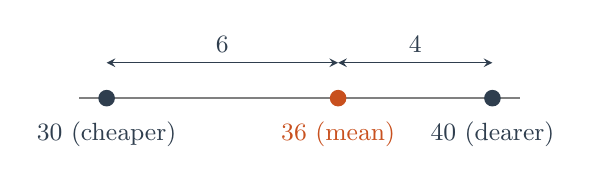
\begin{tikzpicture}[x=0.7cm,font=\small,>=stealth]
\draw[thick,color=gray] (-0.5,0) -- (7.5,0);
\fill[slate] (0,0) circle (3pt);
\fill[ember] (4.2,0) circle (3pt);
\fill[slate] (7,0) circle (3pt);
\node[below=5pt,color=slate] at (0,0) {30 (cheaper)};
\node[below=5pt,color=ember] at (4.2,0) {36 (mean)};
\node[below=5pt,color=slate] at (7,0) {40 (dearer)};
\draw[<->,color=slate] (0,0.45) -- (4.2,0.45) node[midway,above] {6};
\draw[<->,color=slate] (4.2,0.45) -- (7,0.45) node[midway,above] {4};
\end{tikzpicture}\par\nopagebreak\smallskip
{\small The mean 36 is 6 above the cheaper and 4 below the dearer. Quantities go the opposite way: cheaper : dearer $= 4 : 6 = 2 : 3$. There is more of the dearer, so the mean sits nearer it.}
\end{center}

\infobox{Two habits that remove most mistakes}{
\begin{enumerate}
\item \textbf{Name three numbers:} cheaper $a$, dearer $b$, mean $m$. The mean goes in the middle. If it is not between $a$ and $b$, something is swapped.
\item \textbf{The ratio is of quantities, and it is flipped.} The bigger gap belongs to the \emph{smaller} quantity. Check: the mean is nearer the one you use more of.
\end{enumerate}}

\subsection*{Spot-it table}
Read the wording, find the row, jump to the type.
\begin{center}\small\renewcommand{\arraystretch}{1.18}\setlength{\tabcolsep}{7pt}
\begin{tabularx}{\linewidth}{@{}>{\raggedright\arraybackslash}X l >{\raggedright\arraybackslash}X@{}}
\toprule
\textbf{\color{slate}Wording in the question} & \textbf{\color{slate}Type} & \textbf{\color{slate}The one move} \\ \midrule
20 kg at 30 mixed with 30 kg at 40, price? & M1 & total value $\div$ total quantity \\
In what ratio to get a mixture worth 36? & M2 & cross: gaps from the mean \\
How many kg to add to 30 kg of the other? & M3 & ratio, then one part \\
Sold at 42 making 20\% profit & M4 & mixture's cost first, then M2 \\
Three varieties, the first two in equal parts & M5 & blend two into one first \\
20\% solution with 50\% solution, add water & M6 & strength is the price; water is 0\% \\
Two vessels with different milk : water ratios & M7 & percent of milk in each \\
Add water to change the ratio & M8 & the other ingredient is the anchor \\
Draw off and replace with water & M9 & multiply by $1-\frac{\text{drawn}}{\text{total}}$ \\
Milkman adds water, sells at milk's price & M10 & profit $=$ water $\div$ milk \\
Boys' and girls' averages, class average & M11 & group averages are the prices \\
Sells a part at 20\% profit, the rest at? & M12 & profit percents are the prices \\
\bottomrule
\end{tabularx}\end{center}

\subsection{M1. Price of a mixture (weighted mean)}
\spot ``20 kg at 30 a kg mixed with 30 kg at 40 a kg. Price of the mixture?'' ``30 students average 60 and 20 average 70. Average of all?''

\mech
\begin{enumerate}
\item Value of each part = quantity $\times$ price (or students $\times$ average).
\item Total value = add the values.
\item Mean = total value $\div$ total quantity.
\end{enumerate}

\samp 20 kg of rice at 30 a kg is mixed with 30 kg at 40 a kg. What is the price of the mixture per kg?
\begin{enumerate}
\item Values: $20 \times 30 = 600$ and $30 \times 40 = 1200$.
\item Total value: 1800. Total quantity: 50 kg.
\item Price: $1800 \div 50 = 36$ a kg.
\end{enumerate}
\ans{36 a kg. (Between 30 and 40, nearer 40 because there is more of it.)}

\samp 30 students average 60 marks and 20 students average 70. What is the average of all 50?
\begin{enumerate}
\item Marks: $30 \times 60 = 1800$ and $20 \times 70 = 1400$.
\item Total: 3200 marks for 50 students.
\item Average: $3200 \div 50 = 64$.
\end{enumerate}
\ans{64.}

\tryit 15 litres of milk at 24 a litre are mixed with 10 litres at 34 a litre. Price per litre of the mixture?

\subsection{M2. Alligation: the ratio for a target price}
\spot ``In what ratio must rice at 30 a kg and at 40 a kg be mixed to get a mixture worth 36 a kg?''

\mech
\begin{enumerate}
\item Write three numbers: cheaper $a$, dearer $b$, mean $m$.
\item Cheaper's share = dearer $-$ mean, that is $b - m$.
\item Dearer's share = mean $-$ cheaper, that is $m - a$.
\item Cheaper : dearer $= (b - m) : (m - a)$. Simplify.
\end{enumerate}

\subsection{M3. From the ratio to the quantity}
\spot ``How many kg at 40 must be mixed with 30 kg at 30 to get 34 a kg?''

\mech
\begin{enumerate}
\item Alligation (M2) gives the ratio of the two quantities.
\item The quantity you are given is some number of parts. Find one part.
\item Multiply to get the other quantity.
\end{enumerate}

\samp 30 kg of rice at 30 a kg is mixed with some rice at 40 a kg to get 34 a kg. How much rice at 40?
\begin{enumerate}
\item Cheaper : dearer $= (40 - 34) : (34 - 30) = 6 : 4 = 3 : 2$.
\item The cheaper is 3 parts = 30 kg, so 1 part = 10 kg.
\item The dearer is 2 parts: $2 \times 10 = 20$ kg.
\item Check: $(30 \times 30 + 20 \times 40) \div 50 = 1700 \div 50 = 34$.
\end{enumerate}
\ans{20 kg.}

\samp 60 kg of a mixture worth 16 a kg is made from rice at 12 and at 18. How much of each?
\begin{enumerate}
\item Cheaper : dearer $= (18 - 16) : (16 - 12) = 2 : 4 = 1 : 2$.
\item 3 parts = 60 kg, so 1 part = 20 kg.
\item Cheaper: 20 kg. Dearer: 40 kg.
\end{enumerate}
\ans{20 kg at 12, 40 kg at 18.}

\tryit How many litres of milk at 18 a litre must be added to 12 litres at 24 a litre to get a mixture worth 20 a litre?

\subsection{M4. The mean is hidden behind a selling price}
\spot ``Rice costing 30 and 40 is mixed and sold at 42 a kg, making 20\% profit. In what ratio?''

\mech
\begin{enumerate}
\item The mean you need is the \emph{cost} of the mixture, not its selling price.
\item Cost = selling price $\div$ (1 + profit). For a loss, divide by (1 $-$ loss).
\item Then alligate as in M2.
\end{enumerate}

\samp Rice costing 30 and 40 a kg is mixed and sold at 42 a kg, making 20\% profit. In what ratio was it mixed?
\begin{enumerate}
\item Cost of the mixture: $42 \div 1.2 = 35$.
\item Cheaper : dearer $= (40 - 35) : (35 - 30) = 5 : 5$.
\end{enumerate}
\ans{1 : 1.}

\samp Tea costing 40 and 60 a kg is mixed and sold at 54 a kg for 20\% profit. In what ratio?
\begin{enumerate}
\item Cost of the mixture: $54 \div 1.2 = 45$.
\item Cheaper : dearer $= (60 - 45) : (45 - 40) = 15 : 5 = 3 : 1$.
\end{enumerate}
\ans{3 : 1.}

\tryit Rice costing 40 and 50 a kg is mixed and sold at 55 a kg to gain 25\%. In what ratio?

\subsection{M5. Three ingredients}
\spot ``Three kinds cost 20, 30 and 50. The first two are mixed in equal amounts. That blend is mixed with the third to get 36. Ratio?''

\mech
\begin{enumerate}
\item Blend the first two into one ingredient. Find its price.
\item Alligate the blend with the third.
\item Split the blend's share between the first two in their own ratio.
\end{enumerate}

\samp Three kinds cost 20, 30 and 50 a kg. The first two are mixed in equal amounts, and the blend is mixed with the third to get 36 a kg. Find the ratio of the three.
\begin{enumerate}
\item Blend of 20 and 30 in equal amounts: price 25.
\item Blend : third $= (50 - 36) : (36 - 25) = 14 : 11$.
\item Split the blend's 14 parts equally: 7 and 7.
\item Ratio: $7 : 7 : 11$.
\item Check: $(7 \times 20 + 7 \times 30 + 11 \times 50) \div 25 = 900 \div 25 = 36$.
\end{enumerate}
\ans{7 : 7 : 11.}

\sane Without a link between two of them (like ``equal amounts''), three ingredients have many correct answers. The question must give one.

\tryit Three kinds cost 12, 16 and 24 a kg. The first two are mixed in equal amounts, and the blend is mixed with the third to get 18 a kg. Ratio of the three?

\subsection{M6. Solutions of different strength}
\spot ``How many litres of 20\% solution must be mixed with 30 litres of 50\% to get 40\%?'' ``How much water makes 40\% acid into 25\%?''

\mech
\begin{enumerate}
\item The strength (percent) plays the price.
\item Water is 0\%. A pure substance is 100\%.
\item To find a strength: pure content $\div$ total volume (M1).
\item To find a ratio or a quantity: alligation (M2, M3).
\end{enumerate}

\samp 20 litres of a 30\% solution are mixed with 30 litres of a 50\% solution. What is the strength?
\begin{enumerate}
\item Pure content: 30\% of 20 is 6 litres, and 50\% of 30 is 15 litres.
\item Total pure: 21 litres in 50 litres.
\item Strength: $21 \div 50 = 42\%$.
\end{enumerate}
\ans{42\%.}

\samp How many litres of a 20\% solution must be mixed with 30 litres of a 50\% solution to get 40\%?
\begin{enumerate}
\item 20\% : 50\% $= (50 - 40) : (40 - 20) = 10 : 20 = 1 : 2$.
\item The 50\% solution is 2 parts = 30 litres, so 1 part = 15 litres.
\item The 20\% solution is 1 part: 15 litres.
\item Check: $(15 \times 20 + 30 \times 50) \div 45 = 40$.
\end{enumerate}
\ans{15 litres.}

\samp How much water must be added to 20 litres of 40\% acid to make it 25\%?
\begin{enumerate}
\item Water is 0\%. Water : acid $= (40 - 25) : (25 - 0) = 15 : 25 = 3 : 5$.
\item The acid is 5 parts = 20 litres, so 1 part = 4 litres.
\item Water: $3 \times 4 = 12$ litres.
\item Check: 8 litres of acid in 32 litres is 25\%.
\end{enumerate}
\ans{12 litres.}

\tryit How much water must be added to 30 litres of a 60\% acid solution to bring it down to 40\%?

\subsection{M7. Mixing two mixtures}
\spot ``Vessel A has milk : water = 3 : 1, vessel B has 2 : 3. In what ratio should they be mixed to get 1 : 1?''

\mech
\begin{enumerate}
\item Turn each milk : water ratio into the \textbf{percent of milk}.
\item That percent plays the price. The target ratio gives the mean.
\item Alligate as in M2.
\end{enumerate}

\samp Vessel A is milk : water $= 3 : 1$. Vessel B is $2 : 3$. In what ratio should A and B be mixed to get $1 : 1$?
\begin{enumerate}
\item Milk in A: $\tfrac34 = 75\%$. Milk in B: $\tfrac25 = 40\%$. Target: $\tfrac12 = 50\%$.
\item B (lower) : A (higher) $= (75 - 50) : (50 - 40) = 25 : 10 = 5 : 2$.
\item So A : B $= 2 : 5$.
\item Check: 2 litres of A has 1.5 milk and 0.5 water. 5 litres of B has 2 milk and 3 water. Together: 3.5 and 3.5.
\end{enumerate}
\ans{A : B $= 2 : 5$.}

\tryit Vessel A has milk : water $= 4 : 1$. Vessel B has $1 : 4$. In what ratio should A and B be mixed to get $3 : 2$?

\subsection{M8. Adding one ingredient to change the ratio}
\spot ``40 litres of milk and water, 3 : 1. How much water to make it 3 : 2?''

\mech
\begin{enumerate}
\item Find the actual amount of each ingredient.
\item The ingredient you do \emph{not} add stays the same. It is the anchor. Find one part from it.
\item New amount of the other = its new parts $\times$ one part.
\item Amount to add = new amount $-$ old amount.
\end{enumerate}

\samp 40 litres of milk and water are in the ratio 3 : 1. How much water must be added to make it 3 : 2?
\begin{enumerate}
\item Milk: 30 litres. Water: 10 litres.
\item Milk stays the same: 3 parts = 30, so 1 part = 10.
\item New water: $2 \times 10 = 20$ litres.
\item Add: $20 - 10 = 10$ litres.
\end{enumerate}
\ans{10 litres of water.}

\samp 60 litres of milk and water are in the ratio 7 : 3. How much milk must be added to make it 8 : 3?
\begin{enumerate}
\item Milk: 42 litres. Water: 18 litres.
\item Water stays the same: 3 parts = 18, so 1 part = 6.
\item New milk: $8 \times 6 = 48$ litres.
\item Add: $48 - 42 = 6$ litres.
\item Check: $48 : 18 = 8 : 3$.
\end{enumerate}
\ans{6 litres of milk.}

\tryit 50 litres of milk and water are in the ratio 4 : 1. How much water must be added to make it 4 : 3?

\subsection{M9. Draw off and replace}
\spot ``40 litres of pure milk. 8 litres are taken out and replaced with water. This is done once more. How much milk is left?''

\mech
\begin{enumerate}
\item Each time, the fraction that stays is $1 - \dfrac{\text{taken out}}{\text{total}}$.
\item Milk left = milk at the start $\times$ that fraction, once for each time.
\item The amount taken out is of the \emph{mixture}, not of the milk alone.
\end{enumerate}
\textbf{Formula.} Milk left $=$ milk at the start $\times\left(1-\dfrac{y}{x}\right)^{n}$, where $x$ is the total volume, $y$ is taken out each time, and $n$ is the number of times.

\subsection{M10. Profit from adding water}
\spot ``A milkman adds water to milk and sells it at the price of pure milk. The mixture is 20\% water. Profit?''

\mech
\begin{enumerate}
\item He pays only for the milk. He sells all of the mixture at milk's price.
\item His profit is the water.
\item Profit percent = water $\div$ milk $\times$ 100. (Divide by what he paid for: the milk.)
\end{enumerate}

\samp A milkman sells a mixture that is 20\% water at the price of pure milk. What is his profit percent?
\begin{enumerate}
\item Take 100 litres: 80 milk and 20 water.
\item He pays for 80 litres. He is paid for 100 litres.
\item Profit: 20 on a cost of 80.
\item Profit percent: $20 \div 80 \times 100 = 25\%$.
\end{enumerate}
\ans{25\% (not 20\%).}

\tryit A milkman adds 12 litres of water to 80 litres of pure milk and sells the mixture at the cost price of milk. What is his profit percent?

\subsection{M11. Averages as mixtures}
\spot ``Boys average 60, girls average 70, the class averages 64. Ratio of boys to girls?''

\mech
\begin{enumerate}
\item Group averages play the prices.
\item The combined average is the mean.
\item The number of people is the quantity. Alligate as in M2.
\end{enumerate}

\samp Boys average 60 marks, girls average 70, and the class averages 64. Find boys : girls.
\begin{enumerate}
\item Boys : girls $= (70 - 64) : (64 - 60) = 6 : 4 = 3 : 2$.
\end{enumerate}
\ans{3 : 2.}

\samp All employees average 7000. Officers average 15000 and the others 6000. Find officers : others.
\begin{enumerate}
\item Others (lower) : officers (higher) $= (15000 - 7000) : (7000 - 6000) = 8000 : 1000 = 8 : 1$.
\item So officers : others $= 1 : 8$.
\end{enumerate}
\ans{1 : 8. (The mean is near 6000 because there are many more of the others.)}

\tryit A class of 45 averages 40 kg. Boys average 45 kg and girls 36 kg. How many boys are there?

\subsection{M12. Mixed profit percents}
\spot ``He sells one third of his goods at 20\% profit. At what profit must he sell the rest to make 12\% overall?''

\mech
\begin{enumerate}
\item Profit percents play the prices. The overall profit is the mean.
\item The share of the goods (by cost) is the quantity.
\item Quantity at the lower profit : quantity at the higher profit $= (\text{higher} - \text{overall}) : (\text{overall} - \text{lower})$.
\end{enumerate}

\samp He sells one third of his goods at 20\% profit. At what profit must he sell the rest to make 12\% overall?
\begin{enumerate}
\item Call the unknown profit $x$. It must be below 12.
\item The rest (two thirds) is at $x$, one third is at 20. Ratio $2 : 1$.
\item $2 : 1 = (20 - 12) : (12 - x) = 8 : (12 - x)$.
\item So $12 - x = 4$, and $x = 8$.
\item Check: $\tfrac13 \times 20 + \tfrac23 \times 8 = 6\tfrac23 + 5\tfrac13 = 12$.
\end{enumerate}
\ans{8\% profit.}

\samp Half the goods are sold at 10\% profit and half at 4\% loss. What is the overall result?
\begin{enumerate}
\item Equal halves, so take the plain mean.
\item A loss is negative: $(10 + (-4)) \div 2 = 3$.
\end{enumerate}
\ans{3\% profit.}

\tryit A shopkeeper sells $\tfrac35$ of his goods at 10\% profit. At what profit must he sell the rest to make 14\% overall?

\subsection*{Shortcuts to memorise}
\begin{center}\small\renewcommand{\arraystretch}{1.9}\setlength{\tabcolsep}{8pt}
\begin{tabularx}{\linewidth}{@{}>{\raggedright\arraybackslash}X>{\raggedright\arraybackslash}X@{}}
\toprule
\textbf{\color{slate}Idea} & \textbf{\color{slate}Rule} \\ \midrule
Mean of a mixture & total value $\div$ total quantity \\
Alligation & cheaper : dearer $=(b-m):(m-a)$ \\
Strength of a solution & percent is the price; water is 0\%, pure is 100\% \\
Mixture sold at a profit & mixture's cost $=\dfrac{\text{selling price}}{1+\text{profit}}$ \\
Replacement, $n$ rounds & original $\times\left(1-\dfrac{y}{x}\right)^n$ \\
Dilution profit & $\dfrac{\text{water}}{\text{milk}}\times 100$ \\
Average of combined groups & alligation, with member counts as quantities \\
Mixed profit percents & alligation on the percents, with goods by cost as quantities \\
\bottomrule
\end{tabularx}\end{center}

\subsection*{Sanity checks before you mark the option}
\infobox{Ten seconds that save a wrong answer}{
\begin{itemize}
\item The mean lies strictly between the two values. If it does not, you swapped something.
\item The mean is nearer the ingredient you use more of.
\item Put the answer back: total value $\div$ total quantity should give the mean.
\item Replacement: milk left is smaller than before, and you multiplied fractions, not subtracted litres.
\item Ratios in the answer are of quantities, not of prices.
\end{itemize}}

\subsection*{Traps}
\begin{enumerate}
\item \textbf{Mean outside the two values, or cheaper and dearer swapped} (M2). The mean must sit in the middle.
\item \textbf{The ratio read the wrong way round.} The bigger gap goes with the smaller quantity (M2).
\item \textbf{Giving the ratio of prices} instead of the ratio of quantities (M1, M2).
\item \textbf{Ignoring the profit.} When a selling price is given, find the mixture's cost first (M4).
\item \textbf{Three ingredients with no extra condition} have many answers (M5).
\item \textbf{Using the ratio 3 : 1 as strengths 3 and 1.} Convert to percent of milk first: 75\% and 25\% (M7).
\item \textbf{Adding to the wrong thing.} When water is added, milk is the anchor, not the total (M8).
\item \textbf{Replacement done by subtraction.} 40 minus 8 minus 8 is 24, but the answer is 25.6. Multiply the fractions (M9).
\item \textbf{Dilution profit measured on the selling side.} 20\% water gives 25\% profit, not 20\% (M10).
\item \textbf{Using the averages as a ratio.} Alligate on the gaps from the combined average (M11).
\item \textbf{Mixed profit weighted by selling price.} Weight by cost (M12).
\end{enumerate}

\subsection*{Answers to ``Try it''}
\begin{center}\small\renewcommand{\arraystretch}{1.25}\setlength{\tabcolsep}{8pt}
\begin{tabularx}{\linewidth}{@{}l>{\raggedright\arraybackslash}p{3.4cm}>{\raggedright\arraybackslash}X@{}}
\toprule
\textbf{\color{slate}Type} & \textbf{\color{slate}Answer} & \textbf{\color{slate}Working, step by step} \\ \midrule
M1 & 28 a litre & $15 \times 24 + 10 \times 34 = 700$. \newline $700 \div 25 = 28$. \\
M2 & 3 : 2 & $(35 - 26) : (26 - 20) = 9 : 6$. \\
M3 & 24 litres & Cheaper : dearer $= (24 - 20) : (20 - 18) = 2 : 1$. \newline The 12 litres is 1 part, so the cheaper is 2 parts. \\
M4 & 3 : 2 & Cost $55 \div 1.25 = 44$. \newline $(50 - 44) : (44 - 40) = 6 : 4$. \\
M5 & 3 : 3 : 4 & Blend of 12 and 16 is 14. \newline Blend : third $= (24 - 18) : (18 - 14) = 3 : 2 = 6 : 4$. \newline Split the blend's 6 parts equally: 3 and 3. \\
M6 & 15 litres & Water 0\%, acid 60\%, target 40\%. \newline Water : acid $= 20 : 40 = 1 : 2$. \newline Acid 30 litres is 2 parts. \\
M7 & A : B $= 2 : 1$ & A has 80\% milk, B 20\%, target 60\%. \newline B : A $= 20 : 40 = 1 : 2$. \\
M8 & 20 litres & Milk 40, water 10. \newline Milk 4 parts = 40, 1 part 10. New water 30. \\
M9 & 32 litres & Stays $\tfrac{40}{50} = 0.8$ each time. \newline $50 \times 0.8 \times 0.8 = 32$. \\
M10 & 15\% & Water 12, milk 80. \newline $12 \div 80 \times 100 = 15$. \\
M11 & 20 boys & Girls : boys $= (45 - 40) : (40 - 36) = 5 : 4$. \newline 9 parts = 45, 1 part = 5. Boys $4 \times 5$. \\
M12 & 20\% & Rest is $\tfrac25$. Ratio $3 : 2 = (x - 14) : (14 - 10)$. \newline $x - 14 = 6$. \\
\bottomrule
\end{tabularx}\end{center}

\clearpage
\section[Profit and loss (L1--L12)]{Profit and loss (with discount and marked price)}\label{ch:L}
\addtocontents{toc}{\protect\nopagebreak}

\subsection*{The one idea}
Three prices run through every question: the \textbf{cost price} (CP, what the seller paid), the \textbf{marked price} (MP, the label) and the \textbf{selling price} (SP, what the buyer pays). One rule settles most mistakes: \textbf{profit, loss and mark-up percents are out of the CP; a discount percent is out of the MP.}

\begin{center}
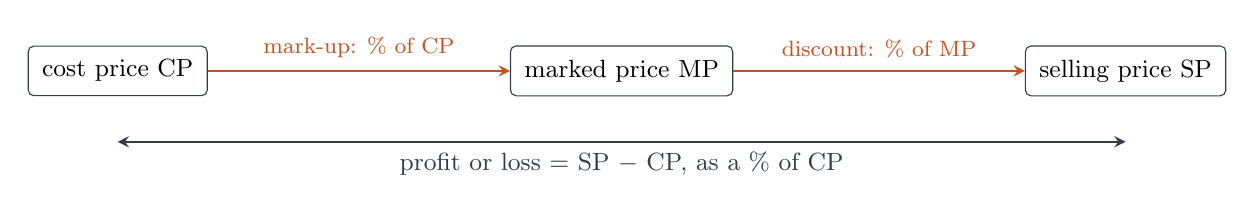
\begin{tikzpicture}[font=\small,>=stealth]
\node[draw=slate,rounded corners=2pt,inner sep=5pt] (a) at (0,0) {cost price CP};
\node[draw=slate,rounded corners=2pt,inner sep=5pt] (b) at (6.4,0) {marked price MP};
\node[draw=slate,rounded corners=2pt,inner sep=5pt] (c) at (12.8,0) {selling price SP};
\draw[->,thick,color=ember] (a) -- (b) node[midway,above=1pt,font=\footnotesize] {mark-up: \% of CP};
\draw[->,thick,color=ember] (b) -- (c) node[midway,above=1pt,font=\footnotesize] {discount: \% of MP};
\draw[<->,thick,color=slate] (0,-0.9) -- (12.8,-0.9) node[midway,below] {profit or loss $=$ SP $-$ CP, as a \% of CP};
\end{tikzpicture}
\end{center}

\infobox{Two habits that remove most mistakes}{
\begin{enumerate}
\item \textbf{Percent of what?} CP for profit, loss and mark-up. MP for discount. Say it before you calculate.
\item \textbf{No number given? Start from 100.} Set the base (CP, or MP for a discount) at 100. It is the percent version of the chairs, and each step becomes easy to follow (L4, L5, L7).
\end{enumerate}}

\subsection*{Spot-it table}
Read the wording, find the row, jump to the type.
\begin{center}\small\renewcommand{\arraystretch}{1.18}\setlength{\tabcolsep}{7pt}
\begin{tabularx}{\linewidth}{@{}>{\raggedright\arraybackslash}X l >{\raggedright\arraybackslash}X@{}}
\toprule
\textbf{\color{slate}Wording in the question} & \textbf{\color{slate}Type} & \textbf{\color{slate}The one move} \\ \midrule
Bought for 800, sold for 920, profit percent? & L1 & profit $\div$ cost \\
Sold at 15\% profit, find the cost (or the price) & L2 & multiply or divide by the multiplier \\
A sells to B, B sells to C & L3 & multiply the multipliers \\
Marked price, discount, profit & L4 & discount on MP, profit on CP \\
At what price must it be marked to earn 20\%? & L5 & work back from the selling price \\
Successive discounts, buy 3 get 1 free & L6 & multiply, or $\frac{\text{free}}{\text{total}}$ \\
Two items, same selling price, one gain, one loss & L7 & loss of $\frac{x^2}{100}\%$ \\
Part sold at 25\% profit, rest at 5\% loss & L8 & weight each part by its cost \\
CP of 15 articles = SP of 12 articles & L9 & $\frac{x-y}{y}\times 100$ \\
Uses a 900 g weight for 1 kg & L10 & error $\div$ weight given \\
20\% of the stock spoils, sells the rest & L11 & whole cost over fewer units \\
Sold at 1200 he loses 20\%; what price gains 15\%? & L12 & find the cost first \\
\bottomrule
\end{tabularx}\end{center}

\subsection{L1. Basics: profit, loss and percent}
\spot ``Bought for 800, sold for 920. Profit percent?'' ``Bought for 4000, spent 500 on repairs, sold for 5400.''

\mech
\begin{enumerate}
\item CP includes every cost to get the item ready to sell (repairs, transport, packing).
\item Profit = SP $-$ CP. Loss = CP $-$ SP.
\item Profit\% = profit $\div$ \textbf{CP} $\times$ 100. Loss\% = loss $\div$ \textbf{CP} $\times$ 100.
\end{enumerate}

\samp Bought for 800, sold for 920. Profit percent?
\begin{enumerate}
\item Profit: $920 - 800 = 120$.
\item Profit\%: $120 \div 800 \times 100 = 15\%$.
\end{enumerate}
\ans{15\% profit.}

\samp Bought for 500, sold for 450. Loss percent?
\begin{enumerate}
\item Loss: $500 - 450 = 50$.
\item Loss\%: $50 \div 500 \times 100 = 10\%$.
\end{enumerate}
\ans{10\% loss.}

\samp Bought for 4000, 500 spent on repairs, sold for 5400. Profit percent?
\begin{enumerate}
\item CP: $4000 + 500 = 4500$.
\item Profit: $5400 - 4500 = 900$.
\item Profit\%: $900 \div 4500 \times 100 = 20\%$.
\end{enumerate}
\ans{20\% profit.}

\samp A shopkeeper's profit is 20\% of his \emph{selling} price. What is it as a percent of cost?
\begin{enumerate}
\item Take SP = 100. Profit = 20, so CP = 80.
\item Profit on cost: $20 \div 80 \times 100 = 25\%$.
\end{enumerate}
\ans{25\%.}

\tryit (a) Bought for 1250, sold for 1500. Profit percent? (b) A scooter is bought for 24000, 2000 is spent on repairs, and it is sold for 23400. Profit or loss percent?

\subsection{L2. SP from CP, and CP from SP}
\spot ``Cost 600, sold at 25\% profit. SP?'' ``Sold for 1155 at 10\% profit. Cost?''

\mech
\begin{enumerate}
\item Multiplier: profit $p\%$ is $1 + \tfrac{p}{100}$. Loss $p\%$ is $1 - \tfrac{p}{100}$.
\item SP = CP $\times$ multiplier.
\item CP = SP $\div$ multiplier. Never take the percent off the SP.
\end{enumerate}

\samp Cost 600, sold at 25\% profit. Selling price?
\begin{enumerate}
\item $600 \times 1.25 = 750$.
\end{enumerate}
\ans{750.}

\samp Sold for 1155 at 10\% profit. Cost price?
\begin{enumerate}
\item $1155 \div 1.1 = 1050$.
\end{enumerate}
\ans{1050.}

\samp Sold for 765 at 15\% loss. Cost price?
\begin{enumerate}
\item $765 \div 0.85 = 900$.
\end{enumerate}
\ans{900.}

\tryit (a) Sold for 1080 at 20\% profit. Cost? (b) Sold for 640 at 20\% loss. Cost?

\subsection{L3. A chain of sellers}
\spot ``A buys for 500 and sells to B at 20\% profit. B sells to C at 10\% profit. What does C pay?''

\mech
\begin{enumerate}
\item Each seller's cost is the previous seller's price.
\item Multiply by each seller's multiplier in turn.
\item To go back, divide by each multiplier in turn.
\end{enumerate}

\samp A buys for 500 and sells to B at 20\% profit. B sells to C at 10\% profit. What does C pay?
\begin{enumerate}
\item B pays: $500 \times 1.2 = 600$.
\item C pays: $600 \times 1.1 = 660$.
\end{enumerate}
\ans{660.}

\samp A buys for 800 and sells to B at 25\% profit. B sells to C at 10\% loss. What does C pay?
\begin{enumerate}
\item B pays: $800 \times 1.25 = 1000$.
\item C pays: $1000 \times 0.9 = 900$.
\end{enumerate}
\ans{900.}

\tryit A sells to B at 25\% profit, and B sells to C at 20\% profit. C pays 750. What did A pay?

\subsection{L4. Marked price and discount}
\spot ``Marked 1000, sold at 20\% discount, cost 640. Profit percent?'' ``Marked 25\% above cost, 10\% discount. Profit percent?''

\mech
\begin{enumerate}
\item The discount is a percent of the \textbf{MP}: SP = MP $\times$ (1 $-$ discount).
\item The profit is a percent of the \textbf{CP}, as in L1.
\item Mark-up and discount together: start from CP = 100 and apply each in turn.
\end{enumerate}

\subsection{L5. What price must be marked?}
\spot ``Cost 900. What should the marked price be to earn 25\% profit after a 10\% discount?''

\mech
\begin{enumerate}
\item SP = CP $\times$ (1 + profit).
\item MP = SP $\div$ (1 $-$ discount).
\end{enumerate}

\samp Cost 900. What marked price gives 25\% profit after a 10\% discount?
\begin{enumerate}
\item SP: $900 \times 1.25 = 1125$.
\item MP: $1125 \div 0.9 = 1250$.
\end{enumerate}
\ans{1250.}

\samp By what percent above cost must goods be marked to earn 20\% profit after a 10\% discount?
\begin{enumerate}
\item CP = 100.
\item SP: $100 \times 1.2 = 120$.
\item MP: $120 \div 0.9 = 133\tfrac13$.
\end{enumerate}
\ans{$33\tfrac13\%$ above cost.}

\tryit Cost 800. What marked price gives 20\% profit after a 4\% discount?

\subsection{L6. Successive discounts}
\spot ``Two discounts of 20\% and 10\%. One equal discount?'' ``Buy 3, get 1 free.''

\mech
\begin{enumerate}
\item Start from MP = 100. Take off each discount in turn, from the new price.
\item Single equal discount = 100 $-$ final price.
\item ``Buy $x$, get $y$ free'': you pay for $x$ and get $x + y$. Discount $= \dfrac{y}{x + y}$.
\end{enumerate}
\textbf{Formula.} Two discounts: $d_1 + d_2 - \dfrac{d_1 \times d_2}{100}$.

\samp Two successive discounts of 20\% and 10\%. What single discount is the same? What is the price on a marked price of 2000?
\begin{enumerate}
\item From 100: less 20\% gives 80.
\item Less 10\% of 80 gives 72.
\item Single discount: $100 - 72 = 28\%$. (Formula: $20 + 10 - 2 = 28$.)
\item On 2000: $2000 \times 0.8 \times 0.9 = 1440$.
\end{enumerate}
\ans{28\%, and the price is 1440.}

\samp Which is better for the buyer: one 30\% discount, or 10\% then 20\%?
\begin{enumerate}
\item One 30\%: he pays 70.
\item 10\% then 20\%: $100 \to 90 \to 72$. He pays 72.
\end{enumerate}
\ans{The single 30\% discount.}

\samp Buy 3, get 1 free. What discount is that?
\begin{enumerate}
\item You pay for 3 and get 4.
\item Discount: $1 \div 4 = 25\%$.
\end{enumerate}
\ans{25\%.}

\tryit Successive discounts of 25\% and 20\%. What single discount is the same?

\subsection{L7. Same selling price, one gain and one loss}
\spot ``Two articles sold at 1200 each, one at 20\% profit, the other at 20\% loss. Overall?''

\mech
\begin{enumerate}
\item Find each cost: CP = SP $\div$ multiplier (L2).
\item Compare the total cost with the total sold.
\end{enumerate}
\textbf{Shortcut.} Same selling price, $x\%$ profit on one and $x\%$ loss on the other: always a \textbf{loss} of $\dfrac{x \times x}{100}\%$.

\samp Two articles are sold at 1200 each. One makes 20\% profit, the other 20\% loss. Overall result?
\begin{enumerate}
\item First cost: $1200 \div 1.2 = 1000$.
\item Second cost: $1200 \div 0.8 = 1500$.
\item Total cost: 2500. Total sold: 2400.
\item Loss: 100. Loss\%: $100 \div 2500 \times 100 = 4\%$.
\item Shortcut check: $20 \times 20 \div 100 = 4$.
\end{enumerate}
\ans{4\% loss.}

\sane The article sold at a loss cost more, so the loss outweighs the gain.

\tryit Two articles are sold at 2400 each, one at 25\% profit and the other at 25\% loss. Overall profit or loss percent?

\subsection{L8. Parts sold at different percents}
\spot ``Goods cost 20000. 40\% sold at 25\% profit, the rest at 5\% loss. Overall?''

\mech
\begin{enumerate}
\item Split the cost into the parts.
\item Profit or loss of each part in money.
\item Net = profits $-$ losses.
\item Overall percent = net $\div$ total cost $\times$ 100.
\end{enumerate}

\samp Goods cost 20000. 40\% are sold at 25\% profit and the rest at 5\% loss. Overall profit percent?
\begin{enumerate}
\item Part one costs 40\% of 20000 = 8000. Profit: 25\% of 8000 = 2000.
\item Part two costs 12000. Loss: 5\% of 12000 = 600.
\item Net: $2000 - 600 = 1400$.
\item Overall: $1400 \div 20000 \times 100 = 7\%$.
\item Quick check: $0.4 \times 25 - 0.6 \times 5 = 10 - 3 = 7$.
\end{enumerate}
\ans{7\% profit.}

\tryit Goods cost 30000. One third is sold at 30\% profit and the rest at 6\% loss. Overall profit or loss, in money and in percent?

\subsection{L9. Cost of some articles = selling price of others}
\spot ``The cost of 15 articles equals the selling price of 12 articles. Profit percent?''

\mech
\begin{enumerate}
\item Let the common amount be the LCM of the two numbers.
\item CP of one article = LCM $\div$ the cost-side number.
\item SP of one article = LCM $\div$ the selling-side number.
\item Compare as in L1.
\end{enumerate}
\textbf{Shortcut.} CP of $x$ = SP of $y$: profit\% $=\dfrac{x - y}{y}\times 100$. Profit if $x > y$, loss if $x < y$.

\samp The cost of 15 articles equals the selling price of 12. Profit percent?
\begin{enumerate}
\item Common amount: LCM of 15 and 12 is 60.
\item CP of one: $60 \div 15 = 4$. SP of one: $60 \div 12 = 5$.
\item Profit: 1 on 4, which is 25\%.
\item Shortcut check: $(15 - 12) \div 12 = 25\%$.
\end{enumerate}
\ans{25\% profit.}

\samp The cost of 12 articles equals the selling price of 15. Profit or loss?
\begin{enumerate}
\item Shortcut: $(12 - 15) \div 15 \times 100 = -20$.
\end{enumerate}
\ans{20\% loss.}

\tryit The cost of 18 articles equals the selling price of 15 articles. Profit percent?

\subsection{L10. False weights}
\spot ``He sells at cost price but uses a 900 g weight for 1 kg. Gain percent?''

\mech
\begin{enumerate}
\item The customer pays for the true weight (1000 g) but gets the false weight.
\item Gain = true $-$ false.
\item Gain\% = gain $\div$ \textbf{false weight} $\times$ 100. (He paid only for what he gave.)
\end{enumerate}
\textbf{With a profit too.} Overall multiplier = (1 + profit) $\times$ true $\div$ false.

\samp He sells at cost price but uses a 900 g weight for 1 kg. Gain percent?
\begin{enumerate}
\item Gain: $1000 - 900 = 100$ g.
\item Gain\%: $100 \div 900 \times 100 = 11\tfrac19\%$.
\end{enumerate}
\ans{$11\tfrac19\%$.}

\samp The same 900 g weight, and he also adds 10\% to the price. Gain percent?
\begin{enumerate}
\item He charges $1.1 \times 1000 = 1100$ for goods that cost him 900.
\item Gain: $1100 - 900 = 200$. Gain\%: $200 \div 900 \times 100 = 22\tfrac29\%$.
\end{enumerate}
\ans{$22\tfrac29\%$.}

\tryit (a) He uses an 800 g weight for 1 kg and sells at cost price. Gain percent? (b) He also sells at 20\% profit. Overall gain percent?

\subsection{L11. Wastage}
\spot ``Buys 100 kg at 50 a kg. 20\% spoils. At what price must he sell the rest for 20\% profit?''

\mech
\begin{enumerate}
\item Total cost = quantity bought $\times$ price. (He paid for all of it.)
\item Money he wants = total cost $\times$ (1 + profit).
\item Quantity left to sell = bought $-$ wasted.
\item Price per kg = money he wants $\div$ quantity left.
\end{enumerate}

\samp He buys 100 kg at 50 a kg. 20\% spoils. At what price per kg must he sell the rest to make 20\% profit?
\begin{enumerate}
\item Total cost: $100 \times 50 = 5000$.
\item Money he wants: $5000 \times 1.2 = 6000$.
\item Left to sell: $100 - 20 = 80$ kg.
\item Price: $6000 \div 80 = 75$ a kg.
\end{enumerate}
\ans{75 a kg.}

\tryit A grocer buys 200 kg of rice at 30 a kg. 10\% is wasted. He sells the rest at 36 a kg. Profit or loss percent?

\subsection{L12. Two selling prices, find the cost}
\spot ``Sold at 1200 he loses 20\%. At what price would he gain 15\%?'' ``At 540 a loss, at 660 a gain, same percent.''

\mech
\begin{enumerate}
\item Always find the \textbf{cost} first.
\item One price with its percent: CP = SP $\div$ multiplier (L2).
\item Equal loss and gain percents: CP is exactly halfway between the two prices.
\item Two prices with different profit percents: the money gap is the percent gap of CP. CP = money gap $\div$ percent gap.
\end{enumerate}

\samp Sold at 1200 he loses 20\%. At what price would he gain 15\%?
\begin{enumerate}
\item CP: $1200 \div 0.8 = 1500$.
\item New SP: $1500 \times 1.15 = 1725$.
\end{enumerate}
\ans{1725.}

\samp Selling at 540 gives a loss, and at 660 a gain of the same percent. Find the cost.
\begin{enumerate}
\item Halfway: $(540 + 660) \div 2 = 600$.
\item Check: loss 60, gain 60, both 10\% of 600.
\end{enumerate}
\ans{600.}

\samp Had he sold it for 250 more, he would have gained 25\% instead of 15\%. Find the cost.
\begin{enumerate}
\item The extra 250 is the extra $25 - 15 = 10\%$ of CP.
\item CP: $250 \div 0.1 = 2500$.
\end{enumerate}
\ans{2500.}

\tryit (a) Sold for 720 he loses 10\%. At what price would he gain 25\%? (b) Selling at 480 gives a loss and at 600 a gain of the same percent. Find the cost.

\subsection*{Shortcuts to memorise}
\begin{center}\small\renewcommand{\arraystretch}{1.9}\setlength{\tabcolsep}{8pt}
\begin{tabularx}{\linewidth}{@{}>{\raggedright\arraybackslash}X>{\raggedright\arraybackslash}X@{}}
\toprule
\textbf{\color{slate}Idea} & \textbf{\color{slate}Rule} \\ \midrule
Profit or loss percent & $\dfrac{\text{SP}-\text{CP}}{\text{CP}}\times 100$ \\
SP from CP, CP from SP & CP $\times(1\pm\frac{p}{100})$;\quad SP $\div(1\pm\frac{p}{100})$ \\
Discount & SP $=$ MP $\times\left(1-\dfrac{d}{100}\right)$ \\
Two successive discounts & $d_1+d_2-\dfrac{d_1 d_2}{100}$ \\
Buy $x$, get $y$ free & discount $=\dfrac{y}{x+y}$ \\
Same SP, $x\%$ gain and $x\%$ loss & loss of $\dfrac{x^2}{100}\%$ \\
CP of $x$ articles = SP of $y$ & $\dfrac{x-y}{y}\times 100$ \\
False weight & $\dfrac{\text{true}-\text{false}}{\text{false}}\times 100$ \\
Equal loss\% and gain\% at two SPs & CP $=$ midpoint of the two SPs \\
\bottomrule
\end{tabularx}\end{center}

\subsection*{Sanity checks before you mark the option}
\infobox{Ten seconds that save a wrong answer}{
\begin{itemize}
\item Profit and loss percents are out of CP. A discount is out of MP.
\item A profit needs SP above CP. A loss needs SP below CP.
\item Equal gain and loss percents on equal selling prices always end in a loss.
\item A discount is below 100\%, and so is a loss.
\item Put the answer back: start from CP $= 100$ and apply each step. Do you land on the given price?
\end{itemize}}

\subsection*{Traps}
\begin{enumerate}
\item \textbf{Percent on the wrong base.} Profit is out of CP, not SP (L1). A discount is out of MP, not CP (L4).
\item \textbf{Forgetting extra costs.} Repairs and transport belong in the CP (L1).
\item \textbf{Taking the percent off the SP to get the CP.} Divide by the multiplier (L2).
\item \textbf{Adding the mark-up and the discount.} A 25\% mark-up with a 10\% discount is 12.5\%, not 15\% (L4).
\item \textbf{Adding successive discounts.} 20\% then 10\% is 28\%, not 30\% (L6).
\item \textbf{``Buy 3 get 1 free'' read as 33\%.} You get 4 and pay for 3, so the discount is 25\% (L6).
\item \textbf{Equal gain and loss on equal selling prices as break-even.} It is a loss of $\frac{x^2}{100}\%$ (L7).
\item \textbf{Weighting parts by selling price.} Weight by cost (L8).
\item \textbf{CP of $x$ = SP of $y$ upside down.} Check: more articles on the cost side means a profit (L9).
\item \textbf{False weight measured on the true weight.} Divide by the weight actually given (L10).
\item \textbf{Wastage ignored in the cost.} The whole stock was paid for, only part is sold (L11).
\end{enumerate}

\subsection*{Answers to ``Try it''}
\begin{center}\small\renewcommand{\arraystretch}{1.25}\setlength{\tabcolsep}{8pt}
\begin{tabularx}{\linewidth}{@{}l>{\raggedright\arraybackslash}p{3.4cm}>{\raggedright\arraybackslash}X@{}}
\toprule
\textbf{\color{slate}Type} & \textbf{\color{slate}Answer} & \textbf{\color{slate}Working, step by step} \\ \midrule
L1 & (a) 20\% profit \newline (b) 10\% loss & (a) Profit 250. $250 \div 1250$. \newline (b) CP $24000 + 2000 = 26000$. Loss $26000 - 23400 = 2600$. $2600 \div 26000$. \\
L2 & (a) 900 \newline (b) 800 & (a) $1080 \div 1.2$. \newline (b) $640 \div 0.8$. \\
L3 & 500 & $750 \div 1.2 = 625$ (B's cost). \newline $625 \div 1.25 = 500$. \\
L4 & 12\% profit & CP 100, MP 140, SP $140 \times 0.8 = 112$. \\
L5 & 1000 & SP $800 \times 1.2 = 960$. \newline MP $960 \div 0.96 = 1000$. \\
L6 & 40\% & $100 \to 75 \to 60$. \\
L7 & 6.25\% loss & $25 \times 25 \div 100 = 6.25$. \newline (Costs 1920 and 3200, total 5120. Sold 4800.) \\
L8 & Profit of 1800, which is 6\% & Part one costs 10000, profit 3000. \newline Part two costs 20000, loss 1200. \newline Net 1800. $1800 \div 30000 = 6\%$. \\
L9 & 20\% profit & $(18 - 15) \div 15 \times 100$. \\
L10 & (a) 25\% \newline (b) 50\% & (a) $200 \div 800$. \newline (b) $1.2 \times 1000 = 1200$ for goods costing 800. Gain 400 on 800. \\
L11 & 8\% profit & Cost $200 \times 30 = 6000$. \newline Sells $180 \times 36 = 6480$. Profit 480 on 6000. \\
L12 & (a) 1000 \newline (b) 540 & (a) CP $720 \div 0.9 = 800$. $800 \times 1.25 = 1000$. \newline (b) Halfway between 480 and 600. \\
\bottomrule
\end{tabularx}\end{center}

\clearpage
\section[Calendar (C1--C12)]{Calendar (with odd days and weekdays)}\label{ch:C}
\addtocontents{toc}{\protect\nopagebreak}

\subsection*{The one idea}
A week has 7 days, so after any whole number of weeks you are back on the same weekday. Only the \textbf{odd days} matter: the days left over after taking out whole weeks (the remainder when you divide by 7). Number the weekdays Sunday 0, Monday 1, and so on up to Saturday 6, put them on a wheel, and move round it.

\begin{center}
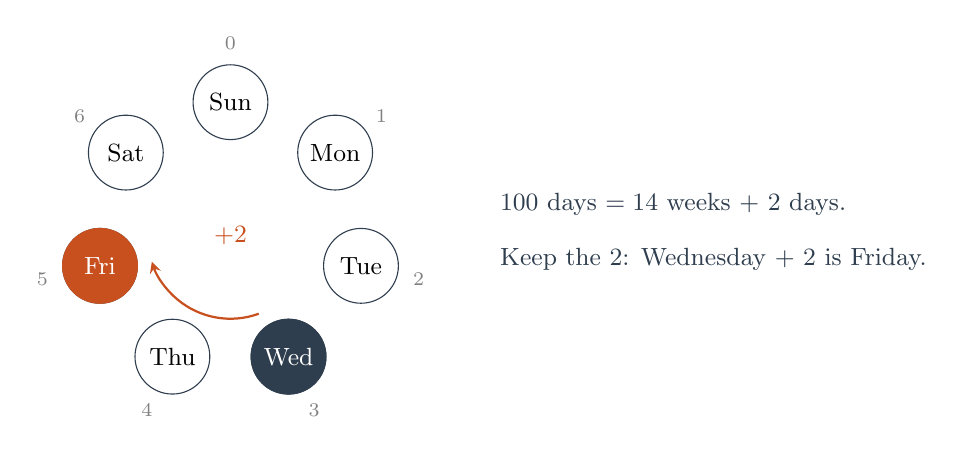
\begin{tikzpicture}[font=\small,>=stealth]
\foreach \k/\nm in {0/Sun,1/Mon,2/Tue,3/Wed,4/Thu,5/Fri,6/Sat}{
  \pgfmathsetmacro{\ang}{90-\k*360/7}
  \node[draw=slate,circle,inner sep=1pt,minimum size=0.95cm] at (\ang:1.7cm) {\nm};
  \node[color=gray,font=\scriptsize] at (\ang:2.45cm) {\k};
}
\node[draw=slate,fill=slate,text=white,circle,inner sep=1pt,minimum size=0.95cm] at (-64.29:1.7cm) {Wed};
\node[draw=ember,fill=ember,text=white,circle,inner sep=1pt,minimum size=0.95cm] at (-167.14:1.7cm) {Fri};
\draw[->,thick,color=ember] (-70:1.05cm) arc[start angle=-70,end angle=-162,radius=1.05cm];
\node[color=ember] at (0,0) {$+2$};
\node[anchor=west,color=slate] at (3.3,0.4) {100 days $=14$ weeks $+\ 2$ days.};
\node[anchor=west,color=slate] at (3.3,-0.3) {Keep the 2: Wednesday $+\ 2$ is Friday.};
\end{tikzpicture}
\end{center}

\infobox{Two habits that remove most mistakes}{
\begin{enumerate}
\item \textbf{Throw away whole weeks.} Divide by 7 and keep the remainder. 100 days is 2 odd days.
\item \textbf{Count the right days.} From a date to the same date next year, a 29 February in between adds one more.
\end{enumerate}}

\subsection*{Spot-it table}
Read the wording, find the row, jump to the type.
\begin{center}\small\renewcommand{\arraystretch}{1.18}\setlength{\tabcolsep}{7pt}
\begin{tabularx}{\linewidth}{@{}>{\raggedright\arraybackslash}X l >{\raggedright\arraybackslash}X@{}}
\toprule
\textbf{\color{slate}Wording in the question} & \textbf{\color{slate}Type} & \textbf{\color{slate}The one move} \\ \midrule
Is 1900 a leap year, how many odd days & C1 & by 4, centuries by 400 \\
Today is Wednesday, what day after 100 days & C2 & divide by 7, keep the remainder \\
Same date next year or the year before & C3 & $+1$, or $+2$ across 29 February \\
On which day was 15 August 1947 & C4 & odd days: centuries, years, days \\
1 January is Monday, what day is 15 August & C5 & month offset table \\
How many Sundays in this month or year & C6 & whole weeks plus extra days \\
Same calendar as 2017 & C7 & add odd days up to a multiple of 7 \\
Which month matches October & C8 & same month offset \\
Sum of the dates of four Wednesdays & C9 & dates differ by 7 \\
Days from 14 February to 3 May, date after 100 days & C10 & rest of the month, whole months \\
The day before yesterday was Thursday & C11 & today is 0, then move \\
Last day of 1900, of a century & C12 & century table 5, 3, 1, 0 \\
\bottomrule
\end{tabularx}\end{center}

\subsection{C1. Leap years and odd days}
\spot ``Is 1900 a leap year?'' ``Leap years from 1901 to 2000?'' ``Odd days in 100 years?''

\mech
\begin{enumerate}
\item \textbf{Leap year:} divisible by 4. But a century year (1900, 2000) must be divisible by \textbf{400}.
\item \textbf{Odd days} = days left after whole weeks. Ordinary year: 1. Leap year: 2.
\item Months: 31 days gives 3 odd days, 30 days gives 2, February 0 (1 in a leap year).
\item Centuries: 100 years give 5 odd days, 200 give 3, 300 give 1, 400 give 0.
\end{enumerate}

\samp Which of 1900, 2000, 2024 and 2100 are leap years?
\begin{enumerate}
\item 1900: a century year, not divisible by 400. Not leap.
\item 2000: divisible by 400. Leap.
\item 2024: divisible by 4. Leap.
\item 2100: a century year, not divisible by 400. Not leap.
\end{enumerate}
\ans{2000 and 2024 only.}

\samp How many leap years from 1901 to 2000? From 2001 to 2100?
\begin{enumerate}
\item 1904 to 2000 in steps of 4: 25 years. 2000 is leap. So 25.
\item 2004 to 2100 in steps of 4: 25 years. But 2100 is not leap. So 24.
\end{enumerate}
\ans{25 and 24.}

\samp How many odd days in 100 years (1601 to 1700)?
\begin{enumerate}
\item 24 leap years and 76 ordinary years.
\item Odd days: $24 \times 2 + 76 \times 1 = 124$.
\item $124 = 17$ weeks $+ 5$.
\item (In 400 years: 97 leap and 303 ordinary give $194 + 303 = 497 = 71$ weeks, so 0.)
\end{enumerate}
\ans{5 odd days.}

\tryit (a) Are 2400 and 2200 leap years? (b) How many leap years are there from 1801 to 1900?

\subsection{C2. Days later, days ago}
\spot ``Today is Wednesday. What day after 100 days?'' ``What day 45 days ago?'' ``The 3rd is a Wednesday. What day is the 26th?''

\mech
\begin{enumerate}
\item Divide the number of days by 7. Keep only the \textbf{remainder}.
\item ``Later'': move forward that many days. ``Ago'': move backward.
\item In one month, days between two dates = the difference of the dates.
\end{enumerate}

\samp Today is Wednesday. What day will it be after 100 days?
\begin{enumerate}
\item $100 = 14 \times 7 + 2$. Remainder 2.
\item Wednesday + 2 = Friday.
\end{enumerate}
\ans{Friday.}

\samp Today is Wednesday. What day was it 45 days ago?
\begin{enumerate}
\item $45 = 6 \times 7 + 3$. Remainder 3.
\item Wednesday $-$ 3 = Sunday.
\end{enumerate}
\ans{Sunday.}

\samp The 3rd of a month is a Wednesday. What day is the 26th?
\begin{enumerate}
\item $26 - 3 = 23$ days later.
\item $23 = 3 \times 7 + 2$. Remainder 2.
\item Wednesday + 2 = Friday.
\end{enumerate}
\ans{Friday.}

\tryit Today is Monday. What day will it be (a) after 59 days, (b) 100 days ago?

\subsection{C3. The same date in another year}
\spot ``15 August 2023 was a Tuesday. What day was 15 August 2024?''

\mech
\begin{enumerate}
\item One year later, the same date moves \textbf{1} day forward.
\item It moves \textbf{2} days if a 29 February lies \emph{between} the two dates.
\item Going back in time, move backward instead.
\end{enumerate}

\samp 15 August 2023 was a Tuesday. What day was 15 August 2024?
\begin{enumerate}
\item 29 February 2024 lies between the two dates. Move 2.
\item Tuesday + 2 = Thursday.
\end{enumerate}
\ans{Thursday.}

\samp 15 August 2023 was a Tuesday. What day was 15 August 2022?
\begin{enumerate}
\item No 29 February between 15 August 2022 and 15 August 2023. Move 1.
\item Going back: Tuesday $-$ 1 = Monday.
\end{enumerate}
\ans{Monday.}

\samp 15 August 2024 is a Thursday. In which year is 15 August next a Thursday?
\begin{enumerate}
\item Moves: 2025 +1, 2026 +1, 2027 +1, 2028 +2 (29 February 2028 is between), 2029 +1, 2030 +1.
\item Total: 7, a whole week.
\end{enumerate}
\ans{2030.}

\tryit 26 January 2023 was a Thursday. What day will 26 January 2025 be?

\subsection{C4. Day of the week for any date}
\spot ``On which day was 15 August 1947?''

\mech
\begin{enumerate}
\item Completed years = year $-$ 1.
\item Odd days from whole blocks: 400 years give 0. Then 100 give 5, 200 give 3, 300 give 1.
\item Odd days from the years left: years + leap years among them (years $\div$ 4, rounded down). Keep the remainder after 7.
\item Odd days in the current year up to the date: 31-day month 3, 30-day month 2, February 0 (1 if leap), plus the date itself.
\item Add all, keep the remainder after 7. 0 = Sunday, 1 = Monday, ..., 6 = Saturday.
\end{enumerate}

\samp On which day was 15 August 1947?
\begin{enumerate}
\item Completed years: $1946 = 1600 + 300 + 46$.
\item 1600 years: 0. 300 years: 1.
\item 46 years: 11 leap years. $46 + 11 = 57 = 8 \times 7 + 1$. That is 1.
\item 1947 to the end of July: $3 + 0 + 3 + 2 + 3 + 2 + 3 = 16$, which is 2.
\item Plus 15 August: 15 is 1. So this year gives $2 + 1 = 3$.
\item Total: $0 + 1 + 1 + 3 = 5$. 5 is Friday.
\end{enumerate}
\ans{Friday.}

\samp On which day was 26 January 1950?
\begin{enumerate}
\item Completed years: $1949 = 1600 + 300 + 49$.
\item 1600 years: 0. 300 years: 1.
\item 49 years: 12 leap years. $49 + 12 = 61 = 8 \times 7 + 5$. That is 5.
\item 26 January: 26 is 5.
\item Total: $0 + 1 + 5 + 5 = 11$, which is 4. 4 is Thursday.
\end{enumerate}
\ans{Thursday.}

\samp On which day was 15 August 2024 (a leap year)?
\begin{enumerate}
\item Completed years: $2023 = 2000 + 23$.
\item 2000 years: 0.
\item 23 years: 5 leap years. $23 + 5 = 28$, which is 0.
\item 2024 to the end of July: $3 + 1 + 3 + 2 + 3 + 2 + 3 = 17$, which is 3.
\item Plus 15: 1. Total: $0 + 0 + 3 + 1 = 4$. 4 is Thursday.
\end{enumerate}
\ans{Thursday.}

\sane Test the method on dates you know: 1 January 2000 was a Saturday. 15 August 1947 was a Friday.

\tryit On which day was (a) 1 January 1901, (b) 14 February 2013?

\subsection{C5. Day of any date from 1 January}
\spot ``1 January 2024 was a Monday. What day was 15 August 2024?''

\mech
\begin{enumerate}
\item Find the month's offset in the table.
\item Day = day of 1 January + month's offset + (date $-$ 1).
\item Keep the remainder after 7.
\end{enumerate}

\subsection{C6. How many times does a weekday occur?}
\spot ``How many Sundays in a 31-day month that starts on a Saturday?'' ``How many Tuesdays in a leap year that starts on a Tuesday?''

\mech
\begin{enumerate}
\item Every weekday occurs once in each full week.
\item The extra days (table) are the \emph{first} few days of the month or year.
\item Those weekdays occur one more time.
\end{enumerate}

\subsection{C7. When does a calendar repeat?}
\spot ``The calendar of 2017 is the same as the calendar of which later year?''

\mech
\begin{enumerate}
\item Two years share a calendar when both conditions hold:
\item (1) both are leap, or both are ordinary;
\item (2) the odd days from the first year up to (not including) the second add up to a multiple of 7.
\item Add year by year (ordinary 1, leap 2) until both hold.
\item A leap year usually repeats after 28 years.
\end{enumerate}

\samp Which later year has the same calendar as 2017?
\begin{enumerate}
\item Running total: 2017: 1, 2018: 2, 2019: 3, 2020 (leap): 5, 2021: 6, 2022: 7.
\item The total reaches 7 after 2022.
\item The next year, 2023, is ordinary like 2017.
\end{enumerate}
\ans{2023.}

\samp Which later year has the same calendar as 2022?
\begin{enumerate}
\item The total reaches 7 after 2027. But 2028 is leap, so it does not match.
\item Keep going. The total reaches 14 after 2032.
\item 2033 is ordinary like 2022.
\end{enumerate}
\ans{2033.}

\samp Which later year has the same calendar as the leap year 2024?
\begin{enumerate}
\item 28 years hold 7 leap years: $28 + 7 = 35$, a multiple of 7.
\item $2024 + 28 = 2052$, which is leap too.
\end{enumerate}
\ans{2052.}

\tryit Which later year has the same calendar as (a) 2025, (b) 2020?

\subsection{C8. Months that match}
\spot ``Which month has the same calendar as October in an ordinary year?''

\mech
\begin{enumerate}
\item Two months start on the same weekday when their offsets (C5 table) are equal.
\item Group the months by offset (table below).
\end{enumerate}

\subsection{C9. Dates of the same weekday}
\spot ``The four Wednesdays of a month add up to 66. Date of the first?'' ``The second Monday is the 12th. What day is the 1st?''

\mech
\begin{enumerate}
\item The same weekday comes every \textbf{7} days.
\item Call the first one $a$. The others are $a + 7$, $a + 14$, $a + 21$.
\item To find the 1st of the month, count back from the first one.
\end{enumerate}

\samp The four Wednesdays of a month add up to 66. What is the date of the first?
\begin{enumerate}
\item $a + (a + 7) + (a + 14) + (a + 21) = 4a + 42$.
\item $4a + 42 = 66$, so $4a = 24$ and $a = 6$.
\item The Wednesdays are 6, 13, 20, 27.
\end{enumerate}
\ans{The 6th.}

\samp The second Monday of a month is the 12th. What day is the 1st?
\begin{enumerate}
\item The first Monday is $12 - 7 = 5$.
\item Count back: 4th Sunday, 3rd Saturday, 2nd Friday, 1st Thursday.
\end{enumerate}
\ans{Thursday.}

\samp The 20th of a month is a Friday. Which dates are Sundays?
\begin{enumerate}
\item Friday + 2 = Sunday, so the 22nd is a Sunday.
\item Step by 7: 1, 8, 15, 22, 29.
\end{enumerate}
\ans{1, 8, 15, 22 and 29.}

\tryit (a) Three Sundays in a row add up to 45. What is the date of the first? (b) The 9th of a month is a Tuesday. What day is the 1st?

\subsection{C10. Counting days between dates}
\spot ``How many days from 14 February to 3 May?'' ``What date is 100 days after 15 January?''

\mech
\begin{enumerate}
\item Days left in the first month + every whole month between + days into the last month.
\item This leaves out the start date and counts the end date. If both ends count, add 1.
\item In a leap year February has 29 days.
\end{enumerate}

\samp How many days from 14 February to 3 May (an ordinary year)?
\begin{enumerate}
\item Rest of February: $28 - 14 = 14$.
\item March: 31. April: 30.
\item Into May: 3.
\item Total: $14 + 31 + 30 + 3 = 78$.
\end{enumerate}
\ans{78 days.}

\samp What date is 100 days after 15 January (an ordinary year)?
\begin{enumerate}
\item Rest of January: $31 - 15 = 16$. Left: $100 - 16 = 84$.
\item February (28): left $84 - 28 = 56$.
\item March (31): left $56 - 31 = 25$.
\item 25 days into April.
\end{enumerate}
\ans{25 April.}

\tryit (a) How many days from 20 March to 5 June (an ordinary year)? (b) What date is 60 days after 10 December 2022?

\subsection{C11. Yesterday and tomorrow puzzles}
\spot ``The day before yesterday was Thursday. What day will it be three days after tomorrow?''

\mech
\begin{enumerate}
\item Call today 0.
\item Yesterday is $-1$, the day before yesterday $-2$. Tomorrow is $+1$, the day after tomorrow $+2$.
\item First find today. Then move from today.
\end{enumerate}

\samp The day before yesterday was Thursday. What day is three days after tomorrow?
\begin{enumerate}
\item Today = Thursday + 2 = Saturday.
\item Tomorrow = Sunday.
\item Three days after that = Wednesday.
\end{enumerate}
\ans{Wednesday.}

\samp The day after tomorrow is Sunday. What was the day before yesterday?
\begin{enumerate}
\item Today = Sunday $-$ 2 = Friday.
\item The day before yesterday = Friday $-$ 2 = Wednesday.
\end{enumerate}
\ans{Wednesday.}

\tryit (a) The day before yesterday was Tuesday. What will the day after tomorrow be? (b) The day after tomorrow is Monday. What day was it three days before yesterday?

\subsection{C12. The last day of a century}
\spot ``On which day was 31 December 1900?'' ``Which weekdays can never end a century?''

\mech
\begin{enumerate}
\item Take out 400-year blocks (0 odd days).
\item The centuries left give 100: 5, 200: 3, 300: 1.
\item Read the weekday from the table.
\end{enumerate}

\subsection*{Shortcuts to memorise}
\begin{center}\small\renewcommand{\arraystretch}{1.9}\setlength{\tabcolsep}{8pt}
\begin{tabularx}{\linewidth}{@{}>{\raggedright\arraybackslash}X>{\raggedright\arraybackslash}X@{}}
\toprule
\textbf{\color{slate}Idea} & \textbf{\color{slate}Rule} \\ \midrule
Leap year & divisible by 4; century years by 400 \\
Odd days & ordinary year 1, leap year 2; 31-day month 3, 30-day month 2 \\
Centuries & 100 years: 5, 200: 3, 300: 1, 400: 0 \\
Weekday codes & Sunday 0, Monday 1, ..., Saturday 6 \\
Same date next year & $+1$, or $+2$ if 29 February is between \\
Day of 1st of each month (ordinary) & 0, 3, 3, 6, 1, 4, 6, 2, 5, 0, 3, 5 \\
Leap year & add 1 from March onward \\
Extra days & 30-day month 2, 31-day month 3, ordinary year 1, leap year 2 \\
Calendar repeat & same leap type and odd days add to a multiple of 7 \\
Same weekday in a month & dates differ by 7 \\
Last day of a century & Friday, Wednesday, Monday, Sunday \\
\bottomrule
\end{tabularx}\end{center}

\subsection*{Sanity checks before you mark the option}
\infobox{Ten seconds that save a wrong answer}{
\begin{itemize}
\item A remainder after dividing by 7 is always 0 to 6.
\item ``Later'' moves forward round the wheel. ``Ago'' moves backward.
\item A leap day only counts if it lies between the two dates.
\item Check your method on a date you know: 15 August 1947 was a Friday, 26 January 1950 a Thursday, 1 January 2000 a Saturday.
\item After February, the offset in a leap year is 1 more than in an ordinary year.
\end{itemize}}

\subsection*{Traps}
\begin{enumerate}
\item \textbf{Century years treated as leap by the ``divisible by 4'' rule.} 1900 and 2100 are not leap (C1).
\item \textbf{Using the whole number of days} instead of the remainder after weeks (C2).
\item \textbf{Moving the wrong way for ``ago''} (C2).
\item \textbf{A leap day that is not between the dates.} 29 February 2024 counts for 15 August 2023 to 15 August 2024 ($+2$), but not for 15 January 2023 to 15 January 2024 ($+1$), because it comes after 15 January 2024 (C3).
\item \textbf{Counting the year of the date as completed.} Use year $-$ 1 (C4).
\item \textbf{Leaving out the date itself.} The days of the current year include the date (C4).
\item \textbf{Using the leap-year offset in January or February} (C5).
\item \textbf{Counting the extra days from the wrong end.} The extra days are the first days of the month or year (C6).
\item \textbf{Calling two years the same when one is leap} and the other is not (C7).
\item \textbf{Equal start days read as equal months.} February and March start alike but differ in length (C8).
\item \textbf{Off by one when counting days between dates.} Decide whether both ends count (C10).
\item \textbf{Century counted from 1901 to 2000} instead of by 400-year blocks (C12).
\end{enumerate}

\subsection*{Answers to ``Try it''}
\begin{center}\small\renewcommand{\arraystretch}{1.25}\setlength{\tabcolsep}{8pt}
\begin{tabularx}{\linewidth}{@{}l>{\raggedright\arraybackslash}p{3.4cm}>{\raggedright\arraybackslash}X@{}}
\toprule
\textbf{\color{slate}Type} & \textbf{\color{slate}Answer} & \textbf{\color{slate}Working, step by step} \\ \midrule
C1 & (a) 2400 is leap, 2200 is not \newline (b) 24 & (a) 400 divides 2400 but not 2200. \newline (b) 1804 to 1900 in fours is 25, but 1900 is not leap. \\
C2 & (a) Thursday \newline (b) Saturday & (a) $59 = 8 \times 7 + 3$. Monday + 3. \newline (b) $100 = 14 \times 7 + 2$. Monday $-$ 2. \\
C3 & Sunday & 2023 to 2024: +1. 2024 to 2025 crosses 29 Feb 2024: +2. \newline Thursday + 3. \\
C4 & (a) Tuesday \newline (b) Thursday & (a) $1900 = 1600 + 300$ gives 1. 1 January gives 1. Total 2. \newline (b) $2012 = 2000 + 12$: $12 + 3 = 15$ gives 1. January 31 and 14 February: $31 + 14 = 45$ gives 3. Total 4. \\
C5 & Thursday & October's offset (ordinary) 0. Date $-$ 1 = 1. \newline Wednesday + 1. \\
C6 & (a) 4 \newline (b) 53 & (a) 2 extra days: Thursday and Friday. Saturday stays at 4. \newline (b) 1 extra day: Friday. \\
C7 & (a) 2031 \newline (b) 2048 & (a) 2025 to 2030: $1 + 1 + 1 + 2 + 1 + 1 = 7$. 2031 is ordinary. \newline (b) Leap year: add 28. \\
C8 & (a) December \newline (b) July & (a) Leap year: September and December both 6. \newline (b) Ordinary year: April and July both 6. \\
C9 & (a) the 8th \newline (b) Monday & (a) $3a + 21 = 45$, so $a = 8$. \newline (b) The 2nd is a Tuesday, so the 1st is a Monday. \\
C10 & (a) 77 days \newline (b) 8 February 2023 & (a) $11 + 30 + 31 + 5 = 77$. \newline (b) 21 to the end of December, 31 in January: 52. Then 8 more. \\
C11 & (a) Saturday \newline (b) Tuesday & (a) Today is Thursday. Thursday + 2. \newline (b) Today is Saturday. Yesterday Friday. Friday $-$ 3. \\
C12 & (a) Wednesday \newline (b) Friday & (a) $1800 = 4 \times 400 + 200$: 3. \newline (b) $2100 = 5 \times 400 + 100$: 5. \\
\bottomrule
\end{tabularx}\end{center}

\clearpage
\section[Clocks (K1--K12)]{Clocks (with hands, faulty clocks and chimes)}\label{ch:K}
\addtocontents{toc}{\protect\nopagebreak}

\subsection*{The one idea}
The dial has \textbf{60 minute spaces} round it. The minute hand moves 1 space every minute. The hour hand moves only $\tfrac1{12}$ of a space every minute. So the minute hand \textbf{gains $\tfrac{11}{12}$ of a space every minute} (55 spaces in an hour). Nearly every clock question asks: how many spaces must the minute hand gain?

\begin{center}\small\renewcommand{\arraystretch}{1.18}\setlength{\tabcolsep}{9pt}
\begin{tabular}{@{}lll@{}}
\toprule
\textbf{\color{slate}Hand} & \textbf{\color{slate}Degrees a minute} & \textbf{\color{slate}Minute spaces a minute} \\ \midrule
Minute hand & $6^\circ$ & 1 \\
Hour hand & $0.5^\circ$ & $\tfrac1{12}$ \\
Minute hand gains on hour hand & $5.5^\circ$ & $\tfrac{11}{12}$ \\
\bottomrule
\end{tabular}\end{center}

\begin{center}
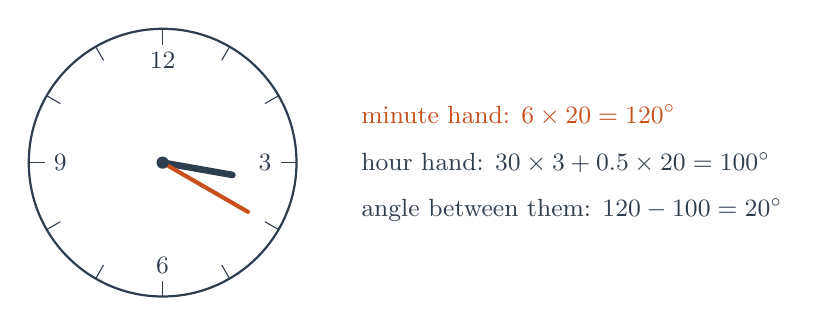
\begin{tikzpicture}[font=\small]
\draw[thick,color=slate] (0,0) circle (1.7cm);
\foreach \a in {0,30,...,330}{
  \draw[color=slate] ({90-\a}:1.5cm) -- ({90-\a}:1.7cm);
}
\node[color=slate] at (90:1.3cm) {12};
\node[color=slate] at (0:1.3cm) {3};
\node[color=slate] at (-90:1.3cm) {6};
\node[color=slate] at (180:1.3cm) {9};
\draw[line width=2.4pt,color=slate,line cap=round] (0,0) -- (-10:0.9cm);
\draw[line width=1.5pt,color=ember,line cap=round] (0,0) -- (-30:1.25cm);
\fill[slate] (0,0) circle (2.2pt);
\node[anchor=west,color=ember] at (2.4,0.6) {minute hand: $6 \times 20 = 120^\circ$};
\node[anchor=west,color=slate] at (2.4,0.0) {hour hand: $30 \times 3 + 0.5 \times 20 = 100^\circ$};
\node[anchor=west,color=slate] at (2.4,-0.6) {angle between them: $120 - 100 = 20^\circ$};
\end{tikzpicture}\par\nopagebreak\smallskip
{\small The clock at 3:20. Angles are measured clockwise from 12.}
\end{center}

\infobox{Two habits that remove most mistakes}{
\begin{enumerate}
\item \textbf{Think in minute spaces.} There are 60 round the dial. At $h$ o'clock the hour hand is $5h$ spaces ahead of the minute hand (count 12 o'clock as 0).
\item \textbf{Ask how many spaces the minute hand must gain.} Then minutes $=$ spaces $\times \tfrac{12}{11}$.
\end{enumerate}}

\subsection*{Spot-it table}
Read the wording, find the row, jump to the type.
\begin{center}\small\renewcommand{\arraystretch}{1.18}\setlength{\tabcolsep}{7pt}
\begin{tabularx}{\linewidth}{@{}>{\raggedright\arraybackslash}X l >{\raggedright\arraybackslash}X@{}}
\toprule
\textbf{\color{slate}Wording in the question} & \textbf{\color{slate}Type} & \textbf{\color{slate}The one move} \\ \midrule
Where are the hands at 3:20 & K1 & $6^\circ$ and $0.5^\circ$ a minute \\
Angle between the hands at 3:15 & K2 & $|30h - 5.5m|$ \\
At what time are the hands at right angles & K3 & spaces the minute hand must gain \\
Hands together or opposite between 4 and 5 & K4 & $\frac{60h}{11}$ \\
How many times a day do the hands coincide & K5 & 11 in 12 hours \\
Clock gains 6 minutes an hour, true time? & K6 & clock time : true time \\
2 minutes slow Monday, 4 minutes fast Thursday & K7 & steady drift \\
When will a faulty clock be right again & K8 & the error reaches 12 hours \\
Hands meet every 64 minutes & K9 & a correct clock: 65 $\frac{5}{11}$ \\
Clock strikes 4 in 6 seconds & K10 & gaps, not strikes \\
Mirror image of 4:20 & K11 & 11:60 minus the time \\
Hands equally far from 12 & K12 & hour angle + minute angle $=360^\circ$ \\
\bottomrule
\end{tabularx}\end{center}

\subsection{K1. Hand speeds and positions}
\spot ``Where are the hands at 3:20?'' ``The hour hand has turned $75^\circ$ since 12. What time is it?''

\mech
\begin{enumerate}
\item Minute hand: $6^\circ$ a minute. Hour hand: $0.5^\circ$ a minute ($30^\circ$ an hour).
\item At $h$ hours $m$ minutes, measured clockwise from 12:
\item Minute hand $= 6m$. Hour hand $= 30h + 0.5m$.
\end{enumerate}

\samp Where are the hands at 3:20?
\begin{enumerate}
\item Minute hand: $6 \times 20 = 120^\circ$.
\item Hour hand: $30 \times 3 + 0.5 \times 20 = 90 + 10 = 100^\circ$.
\end{enumerate}
\ans{Minute hand $120^\circ$, hour hand $100^\circ$ from 12.}

\samp The hour hand has turned $75^\circ$ since 12. What time is it?
\begin{enumerate}
\item The hour hand turns $30^\circ$ an hour.
\item $75 \div 30 = 2.5$ hours.
\end{enumerate}
\ans{2:30.}

\samp How far does each hand turn in 25 minutes?
\begin{enumerate}
\item Minute hand: $6 \times 25 = 150^\circ$.
\item Hour hand: $0.5 \times 25 = 12.5^\circ$.
\end{enumerate}
\ans{$150^\circ$ and $12.5^\circ$.}

\tryit (a) Where are the two hands at 7:24? (b) How many degrees does the hour hand turn in 40 minutes?

\subsection{K2. Angle between the hands}
\spot ``What is the angle between the hands at 3:15?''

\mech
\begin{enumerate}
\item Angle $= |\,30h - 5.5m\,|$. Use 0 for 12 o'clock.
\item If the answer is more than $180^\circ$, take $360^\circ$ minus it.
\end{enumerate}

\samp What is the angle between the hands at 3:15?
\begin{enumerate}
\item $30 \times 3 = 90$ and $5.5 \times 15 = 82.5$.
\item $90 - 82.5 = 7.5$.
\end{enumerate}
\ans{$7.5^\circ$.}

\samp What is the angle at 4:30?
\begin{enumerate}
\item $30 \times 4 = 120$ and $5.5 \times 30 = 165$.
\item $|120 - 165| = 45$.
\end{enumerate}
\ans{$45^\circ$.}

\samp What is the angle at 10:10?
\begin{enumerate}
\item $30 \times 10 = 300$ and $5.5 \times 10 = 55$.
\item $300 - 55 = 245$. That is more than 180.
\item $360 - 245 = 115$.
\end{enumerate}
\ans{$115^\circ$.}

\sane The hour hand moves too. At 3:15 it is a little past the 3, so the angle is not 0.

\tryit What is the angle between the hands at (a) 7:20, (b) 11:35?

\subsection{K3. The time for a given angle}
\spot ``Between 4 and 5, when are the hands at right angles?'' ``Between 7 and 8, when are they $30^\circ$ apart?''

\mech
\begin{enumerate}
\item Turn the angle into minute spaces: $X = \theta \div 6$. ($90^\circ$ is 15 spaces, $30^\circ$ is 5.)
\item At $h$ o'clock the hour hand is $5h$ spaces ahead.
\item The minute hand must gain $5h - X$ spaces (to be $X$ behind) or $5h + X$ (to be $X$ ahead).
\item If a gain is below 0, add 60. If it is 60 or more, take 60 away.
\item Minutes = spaces gained $\times \tfrac{12}{11}$. Keep only answers under 60.
\end{enumerate}

\samp Between 4 and 5, when are the hands at right angles?
\begin{enumerate}
\item $X = 90 \div 6 = 15$ spaces. $5h = 20$.
\item First gain: $20 - 15 = 5$ spaces. Minutes: $5 \times \tfrac{12}{11} = 5\tfrac5{11}$.
\item Second gain: $20 + 15 = 35$ spaces. Minutes: $35 \times \tfrac{12}{11} = 38\tfrac2{11}$.
\end{enumerate}
\ans{4:05$\tfrac5{11}$ and 4:38$\tfrac2{11}$.}

\samp Between 2 and 3, when are the hands at right angles?
\begin{enumerate}
\item $X = 15$. $5h = 10$.
\item First gain: $10 + 15 = 25$ spaces. Minutes: $25 \times \tfrac{12}{11} = 27\tfrac3{11}$.
\item Second gain: $10 - 15 = -5$. Add 60: 55 spaces. Minutes: $55 \times \tfrac{12}{11} = 60$.
\item 60 minutes is exactly 3:00, not between 2 and 3. Drop it.
\end{enumerate}
\ans{Only 2:27$\tfrac3{11}$.}

\samp Between 1 and 2, when are the hands at right angles?
\begin{enumerate}
\item $X = 15$. $5h = 5$.
\item First gain: $5 + 15 = 20$ spaces. Minutes: $20 \times \tfrac{12}{11} = 21\tfrac9{11}$.
\item Second gain: $5 - 15 = -10$. Add 60: 50 spaces. Minutes: $50 \times \tfrac{12}{11} = 54\tfrac6{11}$.
\end{enumerate}
\ans{1:21$\tfrac9{11}$ and 1:54$\tfrac6{11}$.}

\textbf{Shortcut.} Minutes $= \dfrac{60h \pm 2\theta}{11}$. If an answer comes out negative, add $65\tfrac5{11}$. If it comes out as 60 or more, subtract $65\tfrac5{11}$. Keep only answers from 0 up to just under 60.

\tryit (a) Between 7 and 8, when are the hands $30^\circ$ apart? (b) Between 8 and 9, when are they at right angles?

\subsection{K4. Hands together, hands opposite}
\spot ``Between 4 and 5, when do the hands meet?'' ``When are they in a straight line, pointing opposite ways?''

\mech
\begin{enumerate}
\item \textbf{Together:} the minute hand must gain $5h$ spaces. Minutes $= \dfrac{60h}{11}$.
\item \textbf{Opposite}, for $h$ from 0 to 5: minutes $= \dfrac{60h + 360}{11}$.
\item \textbf{Opposite}, for $h$ from 6 to 11: minutes $= \dfrac{60h - 360}{11}$.
\item The hands do not meet between 11 and 12 (they meet at 12:00). They are not opposite between 5 and 6 (they are at 6:00).
\end{enumerate}

\samp Between 4 and 5, when do the hands meet?
\begin{enumerate}
\item $60 \times 4 \div 11 = 240 \div 11 = 21\tfrac9{11}$.
\end{enumerate}
\ans{4:21$\tfrac9{11}$.}

\samp Between 4 and 5, when are the hands opposite?
\begin{enumerate}
\item $h = 4$ is 5 or less: $(240 + 360) \div 11 = 600 \div 11 = 54\tfrac6{11}$.
\end{enumerate}
\ans{4:54$\tfrac6{11}$.}

\samp Between 8 and 9, when are the hands opposite?
\begin{enumerate}
\item $h = 8$ is 6 or more: $(480 - 360) \div 11 = 120 \div 11 = 10\tfrac{10}{11}$.
\end{enumerate}
\ans{8:10$\tfrac{10}{11}$.}

\tryit (a) Between 7 and 8, when do the hands meet? (b) Between 2 and 3, when are they opposite?

\subsection{K5. How often?}
\spot ``How many times do the hands meet in a day?'' ``How many times are they at right angles?''

\mech
\begin{enumerate}
\item The minute hand gains $5.5^\circ$ a minute.
\item A full lap of $360^\circ$ takes $360 \div 5.5 = 65\tfrac5{11}$ minutes.
\item In 12 hours (720 minutes) that happens 11 times.
\end{enumerate}

\subsection{K6. Fast and slow clocks}
\spot ``A clock gains 6 minutes every hour. Set right at 5 am. What is the true time when it shows 4 pm?''

\mech
\begin{enumerate}
\item In 60 true minutes, a clock that gains $g$ shows $60 + g$. One that loses $l$ shows $60 - l$.
\item So clock time : true time $= (60 \pm g) : 60$.
\item Find the clock time passed since it was set right. Convert it to true time.
\item Add to the time it was set right.
\end{enumerate}

\samp A clock gains 6 minutes every hour. It is set right at 5 am. What is the true time when it shows 4 pm?
\begin{enumerate}
\item Clock time passed: 5 am to 4 pm is 11 hours = 660 minutes.
\item Clock : true $= 66 : 60$.
\item True time passed: $660 \times \tfrac{60}{66} = 600$ minutes = 10 hours.
\item True time: 5 am + 10 hours = 3 pm.
\end{enumerate}
\ans{3 pm.}

\samp A clock loses 10 minutes a day. It is set right at 8 am Monday. What does it show at 8 pm Tuesday?
\begin{enumerate}
\item True time passed: 36 hours.
\item Loss: $10 \times 36 \div 24 = 15$ minutes.
\item It shows 8 pm $-$ 15 minutes.
\end{enumerate}
\ans{7:45 pm.}

\tryit (a) A watch loses 5 minutes every hour. It is set right at 7 am. What does it show at a true 1 pm? (b) A clock gains 12 minutes every hour and is set right at 6 am. What is the true time when it shows 4:24 pm?

\subsection{K7. A steady drift between two readings}
\spot ``2 minutes slow at 8 am Monday, 4 minutes fast at 8 am Thursday. When was it right?''

\mech
\begin{enumerate}
\item Total change in error: slow and fast, add them. Both the same way, subtract.
\item Rate of change = total change $\div$ time between readings.
\item Time to cure the first error = first error $\div$ rate.
\end{enumerate}

\samp A watch is 2 minutes slow at 8 am Monday and 4 minutes fast at 8 am Thursday. When was it right?
\begin{enumerate}
\item Time between: 72 hours.
\item Change: $2 + 4 = 6$ minutes in 72 hours, so 1 minute every 12 hours.
\item To cure 2 minutes: $2 \times 12 = 24$ hours after 8 am Monday.
\end{enumerate}
\ans{8 am Tuesday.}

\samp A watch is 2 minutes slow at noon Sunday and 4 min 48 s fast at 2 pm the next Sunday. When was it right?
\begin{enumerate}
\item Time between: $7 \times 24 + 2 = 170$ hours.
\item Change: $2 + 4.8 = 6.8$ minutes. Rate: $6.8 \div 170 = 0.04$ minute an hour.
\item To cure 2 minutes: $2 \div 0.04 = 50$ hours after noon Sunday.
\end{enumerate}
\ans{2 pm Tuesday.}

\tryit A clock is 5 minutes fast at 6 am Monday and 7 minutes slow at 6 am Wednesday. When was it right?

\subsection{K8. When is a faulty clock right again?}
\spot ``A clock gains 15 minutes a day. After how many days does it show the right time again?''

\mech
\begin{enumerate}
\item A 12-hour dial looks right again after it is 12 hours (720 minutes) off.
\item Time = 720 $\div$ (gain or loss per day, or per hour).
\end{enumerate}

\samp A clock gains 15 minutes a day. When is it right again?
\begin{enumerate}
\item $720 \div 15 = 48$.
\end{enumerate}
\ans{After 48 days.}

\samp A clock loses 4 minutes every hour. When is it right again?
\begin{enumerate}
\item $720 \div 4 = 180$ hours.
\item $180 \div 24 = 7.5$ days.
\end{enumerate}
\ans{After 7 days 12 hours.}

\tryit (a) A watch gains 10 minutes a day. After how many days is it right again? (b) A clock loses 6 minutes every hour. After how many days is it right again?

\subsection{K9. Hands that meet at an odd interval}
\spot ``The hands of a clock meet every 64 minutes of true time. How much does it gain or lose in a day?''

\mech
\begin{enumerate}
\item On a correct clock the hands meet every $65\tfrac5{11}$ minutes.
\item If they meet sooner (in true time), the clock is fast. Later, it is slow.
\item Gain per meeting $= 65\tfrac5{11} - $ the given interval.
\item Meetings in a day $= 1440 \div$ the given interval. Multiply.
\end{enumerate}

\samp The hands meet every 64 minutes of true time. How much does the clock gain or lose in a day?
\begin{enumerate}
\item 64 is less than $65\tfrac5{11}$, so the clock is fast.
\item Gain per meeting: $\tfrac{720}{11} - 64 = \tfrac{16}{11}$ minutes.
\item Meetings in a day: $1440 \div 64 = 22.5$.
\item Gain in a day: $22.5 \times \tfrac{16}{11} = \tfrac{360}{11} = 32\tfrac8{11}$ minutes.
\end{enumerate}
\ans{It gains $32\tfrac8{11}$ minutes a day.}

\tryit The hands meet every 65 minutes of true time. Does the clock gain or lose, and how much in a day?

\subsection{K10. Chimes and strikes}
\spot ``How many strikes in a day?'' ``It takes 6 seconds to strike 4. How long to strike 8?''

\mech
\begin{enumerate}
\item Hour strikes in 12 hours: $1 + 2 + \dots + 12 = 78$. In a day: 156.
\item $n$ strikes have only $n - 1$ \textbf{gaps}.
\item Time = number of gaps $\times$ length of one gap.
\end{enumerate}

\samp How many hour strikes in a day?
\begin{enumerate}
\item $1 + 2 + \dots + 12 = 12 \times 13 \div 2 = 78$.
\item Twice a day: $2 \times 78 = 156$.
\end{enumerate}
\ans{156.}

\samp A clock takes 6 seconds to strike 4. How long to strike 8?
\begin{enumerate}
\item 4 strikes have 3 gaps. One gap: $6 \div 3 = 2$ seconds.
\item 8 strikes have 7 gaps: $7 \times 2 = 14$ seconds.
\end{enumerate}
\ans{14 seconds.}

\tryit (a) A clock takes 10 seconds to strike 6. How long to strike 9? (b) A clock strikes the hours and also once every half hour. How many strikes in a day?

\subsection{K11. Mirror images}
\spot ``A clock in a mirror shows 4:20. What is the real time?''

\mech
\begin{enumerate}
\item Mirror time = \textbf{11:60 minus the time}.
\item Use 0 for 12.
\item It works both ways: mirror of the mirror is the real time.
\end{enumerate}

\samp What is the mirror image of 4:20?
\begin{enumerate}
\item $11{:}60 - 4{:}20 = 7{:}40$.
\end{enumerate}
\ans{7:40.}

\samp What are the mirror images of 7:10, 12:20 and 6:00?
\begin{enumerate}
\item 7:10: $11{:}60 - 7{:}10 = 4{:}50$.
\item 12:20 is 0:20: $11{:}60 - 0{:}20 = 11{:}40$.
\item 6:00: $11{:}60 - 6{:}00 = 5{:}60$, which is 6:00.
\end{enumerate}
\ans{4:50, 11:40 and 6:00.}

\tryit (a) What is the mirror image of 3:25? (b) A clock in a mirror shows 2:30. What is the real time?

\subsection{K12. Hands equally far from 12}
\spot ``Between 4 and 5, when are the hands equally far from 12, one on each side?''

\mech
\begin{enumerate}
\item The two hands' angles from 12 add up to $360^\circ$: $30h + 0.5m + 6m = 360$.
\item Solve: minutes $= \dfrac{720 - 60h}{13}$.
\end{enumerate}

\samp Between 4 and 5, when are the hands equally far from 12?
\begin{enumerate}
\item $(720 - 240) \div 13 = 480 \div 13 = 36\tfrac{12}{13}$.
\item Check: hour hand $120 + 0.5 \times 36\tfrac{12}{13} = 138\tfrac6{13}$. Minute hand $6 \times 36\tfrac{12}{13} = 221\tfrac7{13}$. They add to 360.
\end{enumerate}
\ans{4:36$\tfrac{12}{13}$.}

\samp Between 7 and 8, when are the hands equally far from 12?
\begin{enumerate}
\item $(720 - 420) \div 13 = 300 \div 13 = 23\tfrac1{13}$.
\end{enumerate}
\ans{7:23$\tfrac1{13}$.}

\tryit Between 2 and 3, when are the hands equally far from 12?

\subsection*{Shortcuts to memorise}
\begin{center}\small\renewcommand{\arraystretch}{1.9}\setlength{\tabcolsep}{8pt}
\begin{tabularx}{\linewidth}{@{}>{\raggedright\arraybackslash}X>{\raggedright\arraybackslash}X@{}}
\toprule
\textbf{\color{slate}Idea} & \textbf{\color{slate}Rule} \\ \midrule
Speeds & minute hand $6^\circ$ a min, hour hand $0.5^\circ$ a min, gain $5.5^\circ$ a min \\
Positions & minute hand $6m$, hour hand $30h + 0.5m$ \\
Angle between the hands & $|30h - 5.5m|$, then take the smaller of it and $360 -$ it \\
Time for an angle $\theta$ & $\dfrac{60h \pm 2\theta}{11}$; add $65\frac5{11}$ if negative, subtract it if 60 or more \\
Together, opposite & $\dfrac{60h}{11}$;\quad $\dfrac{60h \pm 360}{11}$ \\
How often (12 hours) & together 11, opposite 11, right angles 22 \\
Gap between events & together or opposite $65\frac5{11}$ min, right angle $32\frac8{11}$ min \\
Faulty clock & clock time : true time $=(60 \pm g) : 60$ \\
Right again & 720 minutes of error (12-hour dial) \\
Strikes & $n$ strikes have $n - 1$ gaps \\
Mirror image & 11:60 minus the time \\
Hands equally far from 12 & $\dfrac{720 - 60h}{13}$ \\
\bottomrule
\end{tabularx}\end{center}

\subsection*{Sanity checks before you mark the option}
\infobox{Ten seconds that save a wrong answer}{
\begin{itemize}
\item Minutes after $h$ o'clock must be between 0 and 60.
\item The angle between the hands is never more than $180^\circ$.
\item At 12:00 the hands are together, at 6:00 opposite, at 3:00 and 9:00 at right angles.
\item Put the time back into $|30h - 5.5m|$. Do you get the angle?
\item The hour hand moves too. It is never exactly on a number except on the hour.
\end{itemize}}

\subsection*{Traps}
\begin{enumerate}
\item \textbf{Treating the hour hand as still} (K1, K2). It moves $0.5^\circ$ a minute.
\item \textbf{Not taking the smaller angle.} 245$^\circ$ means 115$^\circ$ (K2).
\item \textbf{Using $h = 12$ in the angle formula.} Use 0 (K2).
\item \textbf{Giving two answers when there is one.} Between 2 and 3 and between 8 and 9 there is only one right angle (K3).
\item \textbf{Looking for a meeting between 11 and 12.} The hands meet at exactly 12:00 (K4).
\item \textbf{12 meetings in 12 hours.} It is 11 (K5).
\item \textbf{Faulty clocks: mixing clock time and true time.} The ratio is clock : true $=(60 \pm g) : 60$ (K6).
\item \textbf{Per hour and per day mixed up} (K6, K8).
\item \textbf{Right again after 24 hours of error} on a 12-hour dial. It is 12 hours (K8).
\item \textbf{Counting strikes instead of gaps.} 4 strikes have 3 gaps (K10).
\item \textbf{Mirror image of 12:xx or 6:00.} Count 12 as 0 (K11).
\item \textbf{Meeting interval used as a clock interval.} The 64 minutes is true time, the $65\frac5{11}$ is clock time (K9).
\end{enumerate}

\subsection*{Answers to ``Try it''}
\begin{center}\small\renewcommand{\arraystretch}{1.25}\setlength{\tabcolsep}{8pt}
\begin{tabularx}{\linewidth}{@{}l>{\raggedright\arraybackslash}p{3.4cm}>{\raggedright\arraybackslash}X@{}}
\toprule
\textbf{\color{slate}Type} & \textbf{\color{slate}Answer} & \textbf{\color{slate}Working, step by step} \\ \midrule
K1 & (a) minute $144^\circ$, hour $222^\circ$ \newline (b) $20^\circ$ & (a) $6 \times 24 = 144$. $30 \times 7 + 0.5 \times 24 = 222$. \newline (b) $0.5 \times 40 = 20$. \\
K2 & (a) $100^\circ$ \newline (b) $137.5^\circ$ & (a) $|210 - 110| = 100$. \newline (b) $|330 - 192.5| = 137.5$. \\
K3 & (a) 7:32$\frac8{11}$ and 7:43$\frac7{11}$ \newline (b) 8:27$\frac3{11}$ only & (a) $5h = 35$, $X = 5$. Gains 30 and 40 spaces. \newline (b) $5h = 40$, $X = 15$. Gains 25 and 55. 55 spaces is 60 minutes, which is 9:00. \\
K4 & (a) 7:38$\frac2{11}$ \newline (b) 2:43$\frac7{11}$ & (a) $420 \div 11$. \newline (b) $(120 + 360) \div 11 = 480 \div 11$. \\
K5 & (a) 22 \newline (b) $16\frac4{11}$ minutes & (a) 11 in 12 hours. \newline (b) $90 \div 5.5$. \\
K6 & (a) 12:30 pm \newline (b) 2:40 pm & (a) 6 true hours, loses $6 \times 5 = 30$ minutes. \newline (b) Clock passed 10 h 24 min $= 624$ min. $624 \times \tfrac{60}{72} = 520$ min $= 8$ h 40 min after 6 am. \\
K7 & 2 am Tuesday & Change $5 + 7 = 12$ minutes in 48 hours: 1 minute every 4 hours. \newline Cure 5 minutes: 20 hours after 6 am Monday. \\
K8 & (a) 72 days \newline (b) 5 days & (a) $720 \div 10$. \newline (b) $720 \div 6 = 120$ hours. \\
K9 & Gains $10\frac{10}{143}$ minutes a day & $\frac{720}{11} - 65 = \frac5{11}$ per meeting. \newline Meetings: $1440 \div 65$. Multiply: $\frac{1440}{143}$. \\
K10 & (a) 16 seconds \newline (b) 180 & (a) 5 gaps in 10 s, so 2 s a gap. 9 strikes: 8 gaps. \newline (b) $156 + 24$. \\
K11 & (a) 8:35 \newline (b) 9:30 & (a) $11{:}60 - 3{:}25$. \newline (b) $11{:}60 - 2{:}30$. \\
K12 & 2:46$\frac2{13}$ & $(720 - 120) \div 13 = 600 \div 13$. \\
\bottomrule
\end{tabularx}\end{center}

\clearpage
\section[Averages and ages (A1--A12)]{Averages and ages (with totals and age differences)}\label{ch:A}
\addtocontents{toc}{\protect\nopagebreak}

\subsection*{The one idea}
An average is the \textbf{fair share}: if every item were made equal, each would be the average. So total $=$ average $\times$ number of items. Anything that changes an average changes the total first. \textbf{Work with totals, never with averages.}

\begin{center}
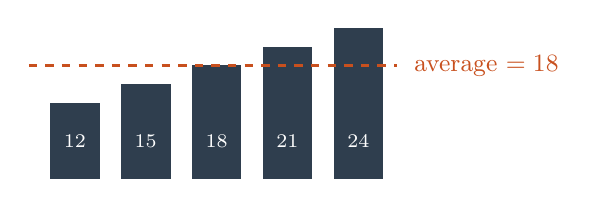
\begin{tikzpicture}[x=0.9cm,y=0.08cm,font=\small]
\foreach \xi/\val in {0/12,1/15,2/18,3/21,4/24}{
  \fill[slate] (\xi,0) rectangle (\xi+0.7,\val);
  \node[color=white,font=\scriptsize] at (\xi+0.35,6) {\val};
}
\draw[dashed,thick,color=ember] (-0.3,18) -- (4.9,18);
\node[anchor=west,color=ember] at (5.0,18) {average $=18$};
\end{tikzpicture}\par\nopagebreak\smallskip
{\small The bars above the line (by 3 and 6) fill exactly the gaps below it (by 3 and 6). Total $=5 \times 18 = 90$.}
\end{center}

\infobox{Two habits that remove most mistakes}{
\begin{enumerate}
\item \textbf{Turn every average into a total} (average $\times$ number), do the adding and subtracting on totals, then divide at the end.
\item \textbf{For ages, the difference between two people never changes.} Everyone gets one year older each year, so a sum of $n$ ages grows by $n$ a year.
\end{enumerate}}

\subsection*{Spot-it table}
Read the wording, find the row, jump to the type.
\begin{center}\small\renewcommand{\arraystretch}{1.18}\setlength{\tabcolsep}{7pt}
\begin{tabularx}{\linewidth}{@{}>{\raggedright\arraybackslash}X l >{\raggedright\arraybackslash}X@{}}
\toprule
\textbf{\color{slate}Wording in the question} & \textbf{\color{slate}Type} & \textbf{\color{slate}The one move} \\ \midrule
Average of 12, 18, 25, 30, 35 & A1 & total $\div$ number; total $=$ average $\times$ number \\
Average of 5, 8, 11, ..., 35; first 20 even numbers & A2 & (first + last) $\div$ 2 \\
A sixth number is added and the average rises & A3 & new total $-$ old total \\
Average of 11 numbers; the first six, the last six & A4 & first total + last total $-$ overall total \\
52 was read as 25, correct average & A5 & fix the total \\
Each number increased by 5, or doubled & A6 & the average does the same \\
Average of 205, 214, 198, 211, 207 & A7 & assumed mean plus average deviation \\
Family's average at the youngest's birth; teacher included & A8 & totals, and years per person \\
A is 12 years older; after 5 years twice as old & A9 & the difference never changes \\
Father 3 times as old; after 10 years twice & A10 & difference $=(k-1)\times$ younger \\
Ratio of ages 4 : 3; six years ago 7 : 5 & A11 & equalise the differences (R4) \\
Sum of ages 60; six years ago 5 times & A12 & the sum falls by 2 per year back \\
\bottomrule
\end{tabularx}\end{center}

\subsection{A1. Average basics: the total}
\spot ``Average of 12, 18, 25, 30, 35.'' ``Average of 6 numbers is 15, five of them add to 70. The sixth?''

\mech
\begin{enumerate}
\item Average = total $\div$ number of items.
\item So total = average $\times$ number of items.
\item A missing item = total needed $-$ total you have.
\end{enumerate}

\samp Find the average of 12, 18, 25, 30, 35.
\begin{enumerate}
\item Total: $12 + 18 + 25 + 30 + 35 = 120$.
\item Average: $120 \div 5 = 24$.
\end{enumerate}
\ans{24.}

\samp The average of 6 numbers is 15. Five of them add up to 70. Find the sixth.
\begin{enumerate}
\item Total of all six: $6 \times 15 = 90$.
\item Sixth: $90 - 70 = 20$.
\end{enumerate}
\ans{20.}

\samp A student scored 70, 78, 74 and 80. What must he score in the fifth test to average 75?
\begin{enumerate}
\item Total needed: $5 \times 75 = 375$.
\item He has: $70 + 78 + 74 + 80 = 302$.
\item He needs: $375 - 302 = 73$.
\end{enumerate}
\ans{73.}

\tryit (a) Average of 8, 14, 17, 21, 25. (b) The average of 4 numbers is 30. Three of them are 25, 28 and 40. Find the fourth.

\subsection{A2. Average of a regular series}
\spot ``Average of 5, 8, 11, ..., 35.'' ``Average of the first 20 even numbers.'' ``6 consecutive even numbers average 25.''

\mech
\begin{enumerate}
\item Same step each time: average = (first + last) $\div$ 2.
\item First $n$ counting numbers: average $(n + 1) \div 2$. First $n$ even numbers: $n + 1$. First $n$ odd numbers: $n$.
\item Odd count of numbers: the average is the middle one. Even count: halfway between the two middle ones.
\item Number of terms = (last $-$ first) $\div$ step + 1.
\end{enumerate}

\samp Find the average of 5, 8, 11, ..., 35.
\begin{enumerate}
\item The step is always 3.
\item Average: $(5 + 35) \div 2 = 20$.
\end{enumerate}
\ans{20. (11 terms, total 220.)}

\samp Find the average of the first 20 even numbers.
\begin{enumerate}
\item First $n$ even numbers average $n + 1$: $20 + 1 = 21$.
\item Check: the numbers are 2 to 40, and $(2 + 40) \div 2 = 21$.
\end{enumerate}
\ans{21.}

\samp Six consecutive even numbers average 25. Find them.
\begin{enumerate}
\item Six numbers: 25 sits between the 3rd and 4th.
\item So the 3rd and 4th are 24 and 26.
\item Count out from there in steps of 2.
\end{enumerate}
\ans{20, 22, 24, 26, 28, 30.}

\tryit (a) Average of 4, 9, 14, ..., 49. (b) Average of the first 30 odd numbers. (c) Seven consecutive numbers average 40. What is the smallest?

\subsection{A3. Adding, removing or replacing an item}
\spot ``5 numbers average 20. A sixth is added and the average becomes 22. Find it.''

\mech
\begin{enumerate}
\item Old total = old average $\times$ old count.
\item New total = new average $\times$ new count.
\item The item added or removed = the difference of the two totals.
\item Replacing: new total = old total $-$ item out + item in.
\end{enumerate}

\samp 5 numbers average 20. A sixth is added and the average becomes 22. Find the sixth.
\begin{enumerate}
\item Old total: $5 \times 20 = 100$.
\item New total: $6 \times 22 = 132$.
\item The sixth number: $132 - 100 = 32$.
\end{enumerate}
\ans{32.}

\samp 8 numbers average 30. One is removed and the other 7 average 28. Which number was removed?
\begin{enumerate}
\item Old total: $8 \times 30 = 240$.
\item New total: $7 \times 28 = 196$.
\item Removed: $240 - 196 = 44$.
\end{enumerate}
\ans{44.}

\samp 10 numbers average 25. One of them, 35, is replaced by 5. New average?
\begin{enumerate}
\item Old total: $10 \times 25 = 250$.
\item New total: $250 - 35 + 5 = 220$.
\item New average: $220 \div 10 = 22$.
\end{enumerate}
\ans{22.}

\tryit (a) 6 numbers average 40. A seventh is added and the average becomes 42. Find it. (b) 9 numbers average 30. One of them, 48, is replaced by 12. New average?

\subsection{A4. Overlapping groups}
\spot ``11 numbers average 50. The first six average 49 and the last six average 52. Find the sixth number.''

\mech
\begin{enumerate}
\item The two groups share an item. Adding the two totals counts it twice.
\item Shared item = first total + last total $-$ overall total.
\end{enumerate}

\samp 11 numbers average 50. The first six average 49 and the last six average 52. Find the sixth number.
\begin{enumerate}
\item First six: $6 \times 49 = 294$.
\item Last six: $6 \times 52 = 312$.
\item All 11: $11 \times 50 = 550$.
\item Sixth: $294 + 312 - 550 = 56$.
\end{enumerate}
\ans{56.}

\samp Monday to Thursday average 40. Tuesday to Friday average 42. Friday is 45. Find Monday.
\begin{enumerate}
\item Monday to Thursday: $4 \times 40 = 160$.
\item Tuesday to Friday: $4 \times 42 = 168$.
\item The difference is Friday $-$ Monday: $168 - 160 = 8$.
\item Monday: $45 - 8 = 37$.
\end{enumerate}
\ans{37.}

\tryit (a) 13 numbers average 42. The first seven average 40 and the last seven average 45. Find the seventh. (b) Monday to Wednesday average 30, and Wednesday to Friday average 35. Wednesday is 32. Find the average of all five days.

\subsection{A5. A wrong reading corrected}
\spot ``10 numbers average 40. 52 was read as 25. Correct average?''

\mech
\begin{enumerate}
\item Wrong total = wrong average $\times$ count.
\item Correct total = wrong total $-$ the wrong value + the right value.
\item Correct average = correct total $\div$ count.
\end{enumerate}

\samp 10 numbers were found to average 40, but 52 had been read as 25. Correct average?
\begin{enumerate}
\item Wrong total: $10 \times 40 = 400$.
\item Correct total: $400 - 25 + 52 = 427$.
\item Correct average: $427 \div 10 = 42.7$.
\end{enumerate}
\ans{42.7.}

\samp 20 numbers average 35. Two were wrong: 51 was noted as 15, and 24 as 42. Correct average?
\begin{enumerate}
\item Wrong total: $20 \times 35 = 700$.
\item First fix: $-15 + 51 = +36$. Second fix: $-42 + 24 = -18$. Net: $+18$.
\item Correct total: $700 + 18 = 718$.
\item Correct average: $718 \div 20 = 35.9$.
\end{enumerate}
\ans{35.9.}

\tryit (a) 15 numbers average 30. One number, 45, was copied as 15. Correct average? (b) 10 numbers average 24, but 38 was entered as 83. Correct average?

\subsection{A6. Changing every number}
\spot ``7 numbers average 20. Each is increased by 5. New average?'' ``Each is multiplied by 4, then 2 is added.''

\mech
\begin{enumerate}
\item Add $k$ to every number: the average goes up by $k$.
\item Multiply every number by $m$: the average is multiplied by $m$.
\item Both: new average = old average $\times m + k$.
\end{enumerate}

\samp 7 numbers average 20. What is the new average if each goes up by 5? If each is doubled?
\begin{enumerate}
\item Up by 5: $20 + 5 = 25$.
\item Doubled: $20 \times 2 = 40$.
\end{enumerate}
\ans{25 and 40.}

\samp 3, 5, 7, 9 average 6. Each is multiplied by 4 and then 2 is added. New average?
\begin{enumerate}
\item $6 \times 4 + 2 = 26$.
\item Check: the numbers become 14, 22, 30, 38, which average 26.
\end{enumerate}
\ans{26.}

\tryit 8 numbers average 25. Each is multiplied by 3, then 7 is taken away. New average?

\subsection{A7. The assumed-mean shortcut}
\spot ``Average of 205, 214, 198, 211, 207.'' Big numbers close together.

\mech
\begin{enumerate}
\item Pick an easy number near them.
\item Write how far each number is above ($+$) or below ($-$) it. Add these.
\item Average = easy number + (sum $\div$ count).
\end{enumerate}

\samp Find the average of 205, 214, 198, 211, 207.
\begin{enumerate}
\item Pick 205.
\item Differences: $0, +9, -7, +6, +2$. Sum: $+10$.
\item $10 \div 5 = 2$.
\item Average: $205 + 2 = 207$.
\end{enumerate}
\ans{207.}

\samp Find the average of 1204, 1212, 1198, 1206.
\begin{enumerate}
\item Pick 1200.
\item Differences: $+4, +12, -2, +6$. Sum: $+20$.
\item $20 \div 4 = 5$.
\item Average: $1200 + 5 = 1205$.
\end{enumerate}
\ans{1205.}

\tryit Find the average of 305, 312, 298, 311, 304.

\subsection{A8. Average ages over time}
\spot ``5 family members average 24. The youngest is 8. Average when the youngest was born?'' ``20 students average 15. With the teacher it is 16.''

\mech
\begin{enumerate}
\item Same people, $t$ years later: the average goes up by $t$.
\item Someone joins or leaves: use totals (A3).
\item At the youngest's birth: leave the youngest out. Everyone else was younger by the youngest's age.
\end{enumerate}

\samp 5 family members average 24 years. The youngest is 8. What was the average of the others when the youngest was born?
\begin{enumerate}
\item Total now: $5 \times 24 = 120$.
\item The other four now: $120 - 8 = 112$.
\item 8 years ago, each of the four was 8 younger: $112 - 4 \times 8 = 80$.
\item Average: $80 \div 4 = 20$.
\end{enumerate}
\ans{20 years.}

\samp 20 students average 15 years. With the teacher, the 21 average 16. How old is the teacher?
\begin{enumerate}
\item With the teacher: $21 \times 16 = 336$.
\item Students only: $20 \times 15 = 300$.
\item Teacher: $336 - 300 = 36$.
\end{enumerate}
\ans{36 years.}

\tryit (a) A family of 4 averages 22. The youngest is 4. What was the average of the other three four years ago? (b) 9 players average 24. With the coach the average is 26. How old is the coach?

\subsection{A9. The age difference never changes}
\spot ``A is 12 years older than B. In 5 years A will be twice as old as B. Present ages?''

\mech
\begin{enumerate}
\item Both get one year older each year. The \textbf{difference stays the same}.
\item If the older is $k$ times the younger, the difference is $(k - 1)$ times the younger.
\item So the younger at that moment = difference $\div (k - 1)$.
\item Move back or forward to the present.
\end{enumerate}

\subsection{A10. ``Times as old'' at two moments}
\spot ``A father is 3 times as old as his son. In 10 years he will be twice as old. Present ages?''

\mech
\begin{enumerate}
\item Let the younger's age now be $s$.
\item At each moment, difference $= (k - 1) \times$ the younger's age then.
\item The two differences are equal. Solve for $s$.
\end{enumerate}

\samp A father is 3 times as old as his son. In 10 years he will be twice as old. Find their ages.
\begin{enumerate}
\item Now: difference $= (3 - 1) \times s = 2s$.
\item In 10 years: difference $= (2 - 1) \times (s + 10) = s + 10$.
\item $2s = s + 10$, so $s = 10$.
\item Father: $3 \times 10 = 30$.
\item Check: in 10 years, 40 and 20.
\end{enumerate}
\ans{Son 10, father 30.}

\samp A mother is 4 times as old as her child. Five years ago she was 7 times as old. Find their ages.
\begin{enumerate}
\item Now: difference $= 3c$.
\item Five years ago: difference $= 6 \times (c - 5) = 6c - 30$.
\item $3c = 6c - 30$, so $3c = 30$ and $c = 10$.
\item Mother: $4 \times 10 = 40$.
\item Check: five years ago, 35 and 5.
\end{enumerate}
\ans{Child 10, mother 40.}

\tryit (a) A man is 5 times as old as his son. In 8 years he will be 3 times as old. Find their ages. (b) A is twice as old as B. Ten years ago A was 3 times as old as B. Find their ages.

\subsection{A11. Ratio of ages across the years}
\spot ``Ages are 4 : 3. Six years ago they were 7 : 5. Present ages?''

\mech
\begin{enumerate}
\item The same years are added to both, so the \textbf{difference} stays the same (as in R4).
\item Scale the two ratios until their differences are equal.
\item One person's change in parts = the number of years. Find one part.
\end{enumerate}

\samp The ages of A and B are 4 : 3. Six years ago they were 7 : 5. Find their ages now.
\begin{enumerate}
\item Differences: $4 - 3 = 1$ and $7 - 5 = 2$.
\item Scale 4 : 3 to 8 : 6, so both differences are 2.
\item A goes from 7 parts (then) to 8 parts (now): 1 part = 6 years.
\item A: $8 \times 6 = 48$. B: $6 \times 6 = 36$.
\item Check: six years ago, $42 : 30 = 7 : 5$.
\end{enumerate}
\ans{A 48, B 36.}

\samp The ages of A and B are 5 : 3. In 10 years they will be 3 : 2. Find their ages now.
\begin{enumerate}
\item Differences: 2 and 1. Scale 3 : 2 to 6 : 4.
\item A goes from 5 parts to 6 parts: 1 part = 10 years.
\item A: 50. B: 30.
\item Check: in 10 years, $60 : 40 = 3 : 2$.
\end{enumerate}
\ans{A 50, B 30.}

\tryit A father and son are 7 : 2 in age. In 4 years they will be 3 : 1. Find their ages now.

\subsection{A12. Sum of ages and a condition}
\spot ``Father and son add up to 60. Six years ago the father was 5 times as old. Present ages?''

\mech
\begin{enumerate}
\item The sum of $n$ people's ages changes by $n$ every year.
\item Find the sum at the moment of the condition.
\item Split that sum in the ratio given. Then move to the present.
\end{enumerate}

\samp A father and son are 60 together. Six years ago the father was 5 times as old as the son. Find their ages now.
\begin{enumerate}
\item Two people, 6 years back: the sum was $60 - 2 \times 6 = 48$.
\item Ratio $5 : 1$ is 6 parts. One part: $48 \div 6 = 8$.
\item Then: son 8, father 40.
\item Now: son 14, father 46. (Sum 60.)
\end{enumerate}
\ans{Son 14, father 46.}

\samp A, B, C are 2 : 3 : 4 in age and add up to 81. In how many years will they add up to 99?
\begin{enumerate}
\item Three people, so the sum grows by 3 a year.
\item Growth needed: $99 - 81 = 18$.
\item Years: $18 \div 3 = 6$.
\end{enumerate}
\ans{6 years.}

\tryit (a) A mother and daughter are 56 together. Four years ago the mother was 7 times as old. Find their ages now. (b) Three brothers are 3 : 5 : 7 in age and add up to 75. In how many years will they add up to 96?

\subsection*{Shortcuts to memorise}
\begin{center}\small\renewcommand{\arraystretch}{1.9}\setlength{\tabcolsep}{8pt}
\begin{tabularx}{\linewidth}{@{}>{\raggedright\arraybackslash}X>{\raggedright\arraybackslash}X@{}}
\toprule
\textbf{\color{slate}Idea} & \textbf{\color{slate}Rule} \\ \midrule
Average and total & total $=$ average $\times$ number \\
Constant step & average $=\dfrac{\text{first}+\text{last}}{2}$ \\
First $n$ numbers & natural $\dfrac{n+1}{2}$, even $n+1$, odd $n$ \\
Item added or removed & difference of the two totals \\
Overlapping groups & total $=$ first $+$ last $-$ shared item \\
A misread number & corrected total $=$ total $-$ wrong $+$ right \\
Add $k$, multiply by $m$ & new average $=$ old $\times\,m + k$ \\
Assumed mean & mean $+\ \dfrac{\text{sum of deviations}}{n}$ \\
Same people, $t$ years later & average $+\,t$ \\
Ages & the difference never changes \\
$k$ times as old & younger $=$ difference $\div\ (k-1)$ \\
Sum of $n$ ages & changes by $n$ each year \\
\bottomrule
\end{tabularx}\end{center}

\subsection*{Sanity checks before you mark the option}
\infobox{Ten seconds that save a wrong answer}{
\begin{itemize}
\item An average lies between the smallest and the largest value.
\item After adding an item above the average, the average goes up. Below the average, it goes down.
\item Put the ages back into the question: do both conditions hold?
\item No age is negative. ``Years ago'' must not be more than the person's age.
\item Averages of groups of different sizes cannot be added. Use totals.
\end{itemize}}

\subsection*{Traps}
\begin{enumerate}
\item \textbf{Averaging averages.} Groups of different sizes need totals (A1, A3).
\item \textbf{The old count used after an item is added or removed} (A3).
\item \textbf{The shared item counted twice} in overlapping groups (A4).
\item \textbf{A correction applied with the wrong sign.} Total $-$ wrong $+$ right (A5).
\item \textbf{Counting terms wrongly.} The number of terms is (last $-$ first) $\div$ step $+$ 1 (A2).
\item \textbf{The wrong count in the assumed-mean division} (A7).
\item \textbf{Counting the youngest before birth.} At the youngest's birth, leave them out (A8).
\item \textbf{Moving only one person's age.} Both change by the same years (A9).
\item \textbf{The ``times as old'' condition applied at the wrong moment} (A10).
\item \textbf{Using the ratio terms as the ages} (A11). Multiply by one part.
\item \textbf{A sum of ages growing by 1 a year.} It grows by the number of people (A12).
\end{enumerate}

\subsection*{Answers to ``Try it''}
\begin{center}\small\renewcommand{\arraystretch}{1.25}\setlength{\tabcolsep}{8pt}
\begin{tabularx}{\linewidth}{@{}l>{\raggedright\arraybackslash}p{3.4cm}>{\raggedright\arraybackslash}X@{}}
\toprule
\textbf{\color{slate}Type} & \textbf{\color{slate}Answer} & \textbf{\color{slate}Working, step by step} \\ \midrule
A1 & (a) 17 \newline (b) 27 & (a) Total 85. $85 \div 5$. \newline (b) Total 120. $120 - 25 - 28 - 40$. \\
A2 & (a) 26.5 \newline (b) 30 \newline (c) 37 & (a) $(4 + 49) \div 2$. \newline (b) First $n$ odd numbers average $n$. \newline (c) The middle is 40, so 37 to 43. \\
A3 & (a) 54 \newline (b) 26 & (a) $7 \times 42 - 6 \times 40 = 294 - 240$. \newline (b) $(270 - 48 + 12) \div 9 = 234 \div 9$. \\
A4 & (a) 49 \newline (b) 32.6 & (a) $280 + 315 - 546$. \newline (b) $(90 + 105 - 32) \div 5 = 163 \div 5$. \\
A5 & (a) 32 \newline (b) 19.5 & (a) $(450 - 15 + 45) \div 15 = 480 \div 15$. \newline (b) $(240 - 83 + 38) \div 10 = 195 \div 10$. \\
A6 & 68 & $25 \times 3 - 7$. \\
A7 & 306 & Pick 300. Differences $+5, +12, -2, +11, +4$, sum 30. \newline $30 \div 5 = 6$. \\
A8 & (a) 24 \newline (b) 44 & (a) Total 88. Others 84. Four years ago $84 - 12 = 72$. $72 \div 3$. \newline (b) $10 \times 26 - 9 \times 24 = 260 - 216$. \\
A9 & (a) A 30, B 10 \newline (b) mother 30, daughter 6 & (a) Five years ago B was $20 \div 4 = 5$. \newline (b) In 6 years the daughter is $24 \div 2 = 12$. \\
A10 & (a) man 40, son 8 \newline (b) A 40, B 20 & (a) $4s = 2(s + 8)$, so $s = 8$. \newline (b) $b = 2(b - 10)$, so $b = 20$. \\
A11 & Father 56, son 16 & Differences 5 and 2. Scale to $14 : 4$ and $15 : 5$ (both 10). \newline Father 14 to 15 parts: 1 part = 4 years. \\
A12 & (a) mother 46, daughter 10 \newline (b) 7 years & (a) Four years ago the sum was 48. 8 parts, daughter 6 then. \newline (b) Sum grows 3 a year. $(96 - 75) \div 3$. \\
\bottomrule
\end{tabularx}\end{center}

\clearpage
\section[Interest (I1--I12)]{Interest (simple and compound)}\label{ch:I}
\addtocontents{toc}{\protect\nopagebreak}

\subsection*{The one idea}
Interest is the price of using someone's money. \textbf{Simple interest} is the same amount every year: a fixed percent of the \emph{original} sum. \textbf{Compound interest} is a fixed percent of the amount at the \emph{start of each year}, so it earns interest on interest. Compound interest is just repeated percent change (P8): multiply by $1+\tfrac{R}{100}$ once a year.

\begin{center}
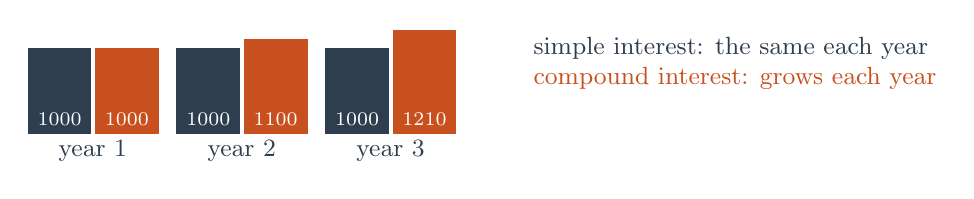
\begin{tikzpicture}[x=0.9cm,y=0.0011cm,font=\small]
\foreach \xa/\sv/\cv in {0/1000/1000,2.1/1000/1100,4.2/1000/1210}{
  \fill[slate] (\xa,0) rectangle (\xa+0.9,\sv);
  \fill[ember] (\xa+0.95,0) rectangle (\xa+1.85,\cv);
  \node[color=white,font=\scriptsize] at (\xa+0.45,170) {\sv};
  \node[color=white,font=\scriptsize] at (\xa+1.4,170) {\cv};
}
\node[color=slate] at (0.92,-190) {year 1};
\node[color=slate] at (3.02,-190) {year 2};
\node[color=slate] at (5.12,-190) {year 3};
\node[anchor=west,color=slate] at (7.0,1000) {simple interest: the same each year};
\node[anchor=west,color=ember] at (7.0,650) {compound interest: grows each year};
\end{tikzpicture}\par\nopagebreak\smallskip
{\small Interest earned each year on 10000 at 10\%. In year 2 the compound sum is 11000, and 10\% of 11000 is 1100.}
\end{center}

\infobox{Two habits that remove most mistakes}{
\begin{enumerate}
\item \textbf{Same units for rate and time.} The rate is per year, so time is in years (8 months is $\tfrac23$ year). Compounded half-yearly: use half the rate and twice the periods.
\item \textbf{Start from 100 when no sum is given.} It is the percent version of the chairs. At 10\% compound for 2 years, 100 becomes 121.
\end{enumerate}}

\subsection*{Spot-it table}
Read the wording, find the row, jump to the type.
\begin{center}\small\renewcommand{\arraystretch}{1.18}\setlength{\tabcolsep}{7pt}
\begin{tabularx}{\linewidth}{@{}>{\raggedright\arraybackslash}X l >{\raggedright\arraybackslash}X@{}}
\toprule
\textbf{\color{slate}Wording in the question} & \textbf{\color{slate}Type} & \textbf{\color{slate}The one move} \\ \midrule
Interest on 5000 at 8\% for 3 years & I1 & $\frac{PRT}{100}$ \\
A sum doubles in 8 years, triples in? & I2 & $R\times T=100(n-1)$ \\
2\% more would give 360 more & I3 & extra percent $\times$ time of the sum \\
A sum split at 6\% and 10\%, total interest & I4 & average rate, then alligation \\
Borrows at 6\%, lends at 8\% & I5 & gain $=$ rate gap $\times P\times T$ \\
10000 at 10\% for 2 years, compound & I6 & multiply by $1+\frac{R}{100}$ each year \\
Compounded half-yearly, quarterly & I7 & half the rate, twice the periods \\
Difference between CI and SI & I8 & $P\left(\frac{R}{100}\right)^2$ for 2 years \\
Sum becomes 12100 in 2 years, 13310 in 3 & I9 & the ratio of amounts a year apart \\
Two equal annual instalments & I10 & divide each by the multiplier \\
2 years 3 months at compound interest & I11 & CI for whole years, SI for the rest \\
CI is 2100 and SI is 2000 for 2 years & I12 & $R=\frac{200\,(\text{CI}-\text{SI})}{\text{SI}}$ \\
\bottomrule
\end{tabularx}\end{center}

\subsection{I1. Simple interest basics}
\spot ``Simple interest on 5000 at 8\% for 3 years.'' ``At what rate does 3000 earn 900 in $2\tfrac12$ years?''

\mech
\begin{enumerate}
\item Simple interest (SI) $= \dfrac{P \times R \times T}{100}$. $P$ is the sum, $R$ the rate a year, $T$ the years.
\item Amount = $P$ + SI.
\item Turned round: $R = \dfrac{100 \times \text{SI}}{P \times T}$, and $T = \dfrac{100 \times \text{SI}}{P \times R}$.
\item Months to years: 6 months $= \tfrac12$ year, 8 months $= \tfrac23$ year.
\end{enumerate}

\samp Find the simple interest and amount on 5000 at 8\% for 3 years.
\begin{enumerate}
\item SI: $5000 \times 8 \times 3 \div 100 = 1200$.
\item Amount: $5000 + 1200 = 6200$.
\end{enumerate}
\ans{SI 1200, amount 6200.}

\samp At what rate does 3000 earn 900 in $2\tfrac12$ years?
\begin{enumerate}
\item $R = 100 \times 900 \div (3000 \times 2.5) = 90000 \div 7500 = 12$.
\end{enumerate}
\ans{12\%.}

\samp Find the interest on 9000 at 8\% for 8 months.
\begin{enumerate}
\item 8 months $= \tfrac23$ year.
\item SI: $9000 \times 8 \times \tfrac23 \div 100 = 480$.
\end{enumerate}
\ans{480.}

\tryit (a) Simple interest on 12000 at $7\tfrac12\%$ for 4 years. (b) In how many years will 8000 become 10400 at 6\% simple interest?

\subsection{I2. A sum doubles, triples}
\spot ``A sum doubles in 8 years at simple interest. When will it triple?''

\mech
\begin{enumerate}
\item A sum becomes $n$ times when the interest is $(n - 1)$ times the sum.
\item That needs $R \times T = 100 \times (n - 1)$.
\item Double: $R \times T = 100$. Triple: 200. Four times: 300.
\end{enumerate}

\samp A sum doubles in 8 years at simple interest. Find the rate, and the time to triple.
\begin{enumerate}
\item Double: $R \times 8 = 100$, so $R = 12.5\%$.
\item Triple: $R \times T = 200$, so $T = 200 \div 12.5 = 16$.
\end{enumerate}
\ans{12.5\%; it triples in 16 years.}

\samp A sum becomes 3 times in 15 years. Find the rate.
\begin{enumerate}
\item Triple: $R \times 15 = 200$.
\item $R = 200 \div 15 = 13\tfrac13$.
\end{enumerate}
\ans{$13\tfrac13\%$.}

\samp At 10\%, how long until a sum becomes 4 times?
\begin{enumerate}
\item Four times: $10 \times T = 300$, so $T = 30$.
\end{enumerate}
\ans{30 years.}

\tryit (a) A sum becomes 5 times in 20 years at simple interest. Find the rate. (b) At 8\% simple interest, how long until a sum doubles?

\subsection{I3. Comparing sums, rates and times}
\spot ``If the rate were 2\% higher, the interest for 3 years would be 360 more. Find the sum.''

\mech
\begin{enumerate}
\item Simple interest goes with $P \times R \times T$.
\item Only the rate changes: extra interest = $P \times$ extra rate $\times T \div 100$.
\item Two cases: work out $P \times R \times T$ for each and compare.
\end{enumerate}

\samp If the rate were 2\% higher, the interest for 3 years would be 360 more. Find the sum.
\begin{enumerate}
\item Extra: $2\% \times 3$ years $= 6\%$ of the sum.
\item 6\% of the sum = 360. So 1\% = 60.
\item Sum: $100 \times 60 = 6000$.
\end{enumerate}
\ans{6000.}

\samp Sums in the ratio 3 : 5 are lent at 8\% for 4 years and at 6\% for 5 years. Ratio of the interests?
\begin{enumerate}
\item First: $3 \times 8 \times 4 = 96$. Second: $5 \times 6 \times 5 = 150$.
\item $96 : 150$. Divide by 6.
\end{enumerate}
\ans{16 : 25.}

\tryit (a) If the rate were 3\% higher, the interest for 2 years would be 450 more. Find the sum. (b) Sums in the ratio 2 : 3 are lent at 5\% for 3 years and 4\% for 5 years. Ratio of the interests?

\subsection{I4. Splitting a sum at two rates}
\spot ``8000 is lent in two parts at 6\% and 10\%. The interest for 2 years is 1280. Find the parts.''

\mech
\begin{enumerate}
\item Average rate $= \dfrac{100 \times \text{total interest}}{P \times T}$.
\item Lower-rate part : higher-rate part $= (\text{higher} - \text{average}) : (\text{average} - \text{lower})$.
\item Split the sum in that ratio.
\end{enumerate}

\samp 8000 is lent in two parts at 6\% and 10\%. The interest for 2 years is 1280. Find the parts.
\begin{enumerate}
\item Average rate: $100 \times 1280 \div (8000 \times 2) = 8\%$.
\item Parts: $(10 - 8) : (8 - 6) = 2 : 2 = 1 : 1$.
\item 4000 and 4000.
\item Check: $4000 \times 6 \times 2 \div 100 = 480$ and $4000 \times 10 \times 2 \div 100 = 800$. Total 1280.
\end{enumerate}
\ans{4000 at 6\% and 4000 at 10\%.}

\samp 9000 is lent at 5\% and 9\%. The interest for 2 years is 1080. Find the parts.
\begin{enumerate}
\item Average rate: $100 \times 1080 \div (9000 \times 2) = 6\%$.
\item Parts: $(9 - 6) : (6 - 5) = 3 : 1$. 4 parts, one part 2250.
\item 6750 at 5\% and 2250 at 9\%.
\item Check: $675 + 405 = 1080$.
\end{enumerate}
\ans{6750 at 5\% and 2250 at 9\%.}

\tryit 12000 is lent in two parts at 5\% and 8\% simple interest. The interest for 1 year is 840. Find the parts.

\subsection{I5. Borrowing and lending}
\spot ``He borrows 5000 at 6\% and lends it at 8\%. What does he gain?''

\mech
\begin{enumerate}
\item He pays one rate and earns another, on the same sum.
\item Gain $= P \times (\text{rate gap}) \times T \div 100$.
\end{enumerate}

\samp He borrows 5000 at 6\% and lends it at 8\%. What does he gain in 1 year? In 3 years?
\begin{enumerate}
\item Rate gap: $8 - 6 = 2\%$.
\item One year: 2\% of 5000 = 100.
\item Three years: $3 \times 100 = 300$.
\end{enumerate}
\ans{100 a year, 300 in 3 years.}

\samp He borrows at 4\% and lends at 6\%, and gains 400 in 4 years. Find the sum.
\begin{enumerate}
\item Gap $\times$ time: $2\% \times 4 = 8\%$ of the sum.
\item 8\% of the sum = 400. So 1\% = 50.
\item Sum: $100 \times 50 = 5000$.
\end{enumerate}
\ans{5000.}

\tryit He borrows at 5\% and lends at $7\tfrac12\%$. He gains 750 in 3 years. Find the sum.

\subsection{I6. Compound interest: the basics}
\spot ``Compound interest on 10000 at 10\% for 2 years.''

\mech
\begin{enumerate}
\item Each year, multiply by $1 + \tfrac{R}{100}$.
\item Amount $= P \times \left(1 + \tfrac{R}{100}\right)^n$ for $n$ years.
\item Compound interest (CI) = amount $-$ $P$.
\end{enumerate}

\samp Find the compound interest on 10000 at 10\% for 2 years, and for 3 years.
\begin{enumerate}
\item Year 1: $10000 \times 1.1 = 11000$.
\item Year 2: $11000 \times 1.1 = 12100$. CI for 2 years: 2100.
\item Year 3: $12100 \times 1.1 = 13310$. CI for 3 years: 3310.
\item (Simple interest for 3 years would be 3000.)
\end{enumerate}
\ans{2100 for 2 years, 3310 for 3 years.}

\samp Find the compound interest on 8000 at 5\% for 3 years.
\begin{enumerate}
\item $8000 \times 1.05 = 8400$.
\item $8400 \times 1.05 = 8820$.
\item $8820 \times 1.05 = 9261$.
\item CI: $9261 - 8000 = 1261$.
\end{enumerate}
\ans{1261.}

\tryit (a) Compound interest on 6250 at 8\% for 2 years. (b) Amount of 5000 at 20\% compound interest for 3 years.

\subsection{I7. Compounded half-yearly or quarterly}
\spot ``Amount on 8000 at 10\% a year for 1 year, compounded half-yearly.''

\mech
\begin{enumerate}
\item Half-yearly: half the rate, twice the number of periods.
\item Quarterly: a quarter of the rate, four times the number of periods.
\item Then multiply once per period, as in I6.
\end{enumerate}

\samp Find the amount on 8000 at 10\% a year for 1 year, compounded half-yearly.
\begin{enumerate}
\item Rate per half-year: 5\%. Periods: 2.
\item $8000 \times 1.05 = 8400$. $8400 \times 1.05 = 8820$.
\item CI: 820. (Yearly it would be 800.)
\end{enumerate}
\ans{8820.}

\samp Find the amount on 16000 at 10\% a year for $1\tfrac12$ years, compounded half-yearly.
\begin{enumerate}
\item Rate per half-year: 5\%. Periods: 3.
\item $16000 \times 1.05 \times 1.05 \times 1.05 = 18522$.
\item CI: 2522.
\end{enumerate}
\ans{18522.}

\samp Find the amount on 10000 at 8\% a year for 6 months, compounded quarterly.
\begin{enumerate}
\item Rate per quarter: 2\%. Periods: 2.
\item $10000 \times 1.02 \times 1.02 = 10404$.
\end{enumerate}
\ans{10404.}

\tryit (a) Amount and compound interest on 20000 at 10\% a year for 1 year, compounded half-yearly. (b) Amount of 5000 at 8\% a year for 6 months, compounded quarterly.

\subsection{I8. The difference between CI and SI}
\spot ``The difference between compound and simple interest for 2 years at 10\% is 50. Find the sum.''

\mech
\begin{enumerate}
\item The difference is interest on interest.
\item 2 years: CI $-$ SI $= P \times \left(\tfrac{R}{100}\right)^2$.
\item 3 years: CI $-$ SI $= P \times \left(\tfrac{R}{100}\right)^2 \times \left(3 + \tfrac{R}{100}\right)$.
\end{enumerate}

\samp CI $-$ SI for 2 years at 10\% is 50. Find the sum.
\begin{enumerate}
\item $\left(\tfrac{10}{100}\right)^2 = 0.01$.
\item $P \times 0.01 = 50$, so $P = 5000$.
\end{enumerate}
\ans{5000.}

\samp CI $-$ SI for 3 years at 10\% is 620. Find the sum.
\begin{enumerate}
\item $0.01 \times (3 + 0.1) = 0.031$.
\item $P \times 0.031 = 620$, so $P = 20000$.
\end{enumerate}
\ans{20000.}

\samp Find CI $-$ SI for 2 years on 8000 at 5\%.
\begin{enumerate}
\item $8000 \times 0.05 \times 0.05 = 20$.
\end{enumerate}
\ans{20.}

\tryit (a) CI $-$ SI for 2 years at 12\% is 144. Find the sum. (b) Find CI $-$ SI for 3 years on 8000 at 5\%.

\subsection{I9. The rate or the time from compound amounts}
\spot ``A sum becomes 12100 in 2 years and 13310 in 3 years. Find the rate.'' ``A sum doubles in 5 years. When is it 8 times?''

\mech
\begin{enumerate}
\item Amounts one year apart: later $\div$ earlier $= 1 + \tfrac{R}{100}$.
\item From the sum and one amount: amount $\div$ sum $= \left(1 + \tfrac{R}{100}\right)^n$. Spot the power.
\item Doubles in $k$ years: 4 times in $2k$, 8 times in $3k$, 16 times in $4k$.
\end{enumerate}

\samp A sum becomes 12100 in 2 years and 13310 in 3 years. Find the rate.
\begin{enumerate}
\item $13310 \div 12100 = 1.1$.
\item So $R = 10\%$.
\end{enumerate}
\ans{10\%.}

\samp 8000 becomes 9261 in 3 years. Find the rate.
\begin{enumerate}
\item $9261 \div 8000 = 1.157625$.
\item That is $1.05 \times 1.05 \times 1.05$. So $R = 5\%$.
\end{enumerate}
\ans{5\%.}

\samp A sum doubles in 5 years. When is it 8 times?
\begin{enumerate}
\item $8 = 2 \times 2 \times 2$: three doublings.
\item $3 \times 5 = 15$.
\end{enumerate}
\ans{15 years.}

\tryit (a) A sum becomes 3456 in 2 years and 4147.2 in 3 years. Find the rate. (b) A sum doubles in 4 years. When is it 16 times?

\subsection{I10. Equal annual instalments}
\spot ``A loan is repaid in two equal yearly instalments of 1210 at 10\% compound interest. What was the loan?''

\mech
\begin{enumerate}
\item \textbf{Compound:} bring each instalment back to today. Divide by the multiplier once for each year it waits. Add them.
\item \textbf{Simple:} after 2 years the lender is owed $P \times (1 + 2r)$. The first instalment counts as $x \times (1 + r)$ (it is paid a year early), the second as $x$.
\end{enumerate}

\samp A loan is repaid in two equal yearly instalments of 1210 at 10\% compound interest. What was the loan?
\begin{enumerate}
\item First instalment, back one year: $1210 \div 1.1 = 1100$.
\item Second, back two years: $1210 \div 1.21 = 1000$.
\item Loan: $1100 + 1000 = 2100$.
\end{enumerate}
\ans{2100.}

\samp A loan of 1750 at 10\% simple interest is repaid in two equal yearly instalments. Find each instalment.
\begin{enumerate}
\item Owed after 2 years: $1750 \times 1.2 = 2100$.
\item $x \times 1.1 + x = 2100$, so $2.1x = 2100$.
\item $x = 1000$.
\end{enumerate}
\ans{1000.}

\tryit What loan is cleared by two equal yearly instalments of 2420 at 10\% compound interest?

\subsection{I11. Changing rates and part years}
\spot ``10\% in year one and 20\% in year two, compounded.'' ``8000 at 10\% for $2\tfrac14$ years.''

\mech
\begin{enumerate}
\item Different rates in different years: multiply each year's own multiplier.
\item A part year: compound for the whole years. Then add simple interest on that amount for the part year.
\end{enumerate}

\samp 10000 grows at 10\% in the first year and 20\% in the second, compounded. Find the amount.
\begin{enumerate}
\item Year 1: $10000 \times 1.1 = 11000$.
\item Year 2: $11000 \times 1.2 = 13200$.
\end{enumerate}
\ans{13200.}

\samp Find the amount on 8000 at 10\% for 2 years 3 months.
\begin{enumerate}
\item 2 whole years: $8000 \times 1.21 = 9680$.
\item 3 months is $\tfrac14$ year. SI on 9680: $9680 \times 10 \times \tfrac14 \div 100 = 242$.
\item Amount: $9680 + 242 = 9922$.
\end{enumerate}
\ans{9922.}

\tryit Find the amount of 5000 at 20\% a year for 2 years 3 months.

\subsection{I12. CI and SI both given for 2 years}
\spot ``For 2 years the compound interest is 2100 and the simple interest is 2000. Find the rate and the sum.''

\mech
\begin{enumerate}
\item Rate: $R = \dfrac{200 \times (\text{CI} - \text{SI})}{\text{SI}}$.
\item Sum: $P = \dfrac{100 \times \text{SI}}{2 \times R}$.
\end{enumerate}

\samp For 2 years, CI is 2100 and SI is 2000. Find the rate and the sum.
\begin{enumerate}
\item $R = 200 \times 100 \div 2000 = 10\%$.
\item $P = 100 \times 2000 \div (2 \times 10) = 10000$.
\end{enumerate}
\ans{10\%, 10000.}

\samp For 2 years, CI is 1040 and SI is 1000. Find the rate and the sum.
\begin{enumerate}
\item $R = 200 \times 40 \div 1000 = 8\%$.
\item $P = 100 \times 1000 \div 16 = 6250$.
\item Check: $6250 \times 1.08 \times 1.08 - 6250 = 1040$.
\end{enumerate}
\ans{8\%, 6250.}

\tryit For 2 years the compound interest on a sum is 820 and the simple interest is 800. Find the rate and the sum.

\subsection*{Shortcuts to memorise}
\begin{center}\small\renewcommand{\arraystretch}{1.9}\setlength{\tabcolsep}{8pt}
\begin{tabularx}{\linewidth}{@{}>{\raggedright\arraybackslash}X>{\raggedright\arraybackslash}X@{}}
\toprule
\textbf{\color{slate}Idea} & \textbf{\color{slate}Rule} \\ \midrule
Simple interest & $\dfrac{P R T}{100}$;\quad amount $=P+$ interest \\
$n$ times at simple interest & $R\times T = 100\,(n-1)$ \\
Interest compared & proportional to $P\times R\times T$ \\
Borrow and lend & gain $=\dfrac{P\times\text{rate gap}\times T}{100}$ \\
Compound amount & $P\left(1+\dfrac{R}{100}\right)^n$ \\
Half-yearly, quarterly & $R\div 2$ and $2n$;\quad $R\div 4$ and $4n$ \\
CI $-$ SI, 2 years & $P\left(\dfrac{R}{100}\right)^2$ \\
CI $-$ SI, 3 years & $P\left(\dfrac{R}{100}\right)^2\left(3+\dfrac{R}{100}\right)$ \\
Rate from two amounts & $\dfrac{A_{n+1}}{A_n}-1$ \\
Doubles in $k$ years (compound) & 4 times in $2k$, 8 times in $3k$ \\
CI and SI for 2 years & $R=\dfrac{200\,(\text{CI}-\text{SI})}{\text{SI}}$ \\
\bottomrule
\end{tabularx}\end{center}

\subsection*{Sanity checks before you mark the option}
\infobox{Ten seconds that save a wrong answer}{
\begin{itemize}
\item In the first year, simple and compound interest are the same. After that, compound is larger.
\item Interest is not the amount. Amount $=$ sum $+$ interest.
\item The rate and the time are in the same units. Months have been turned into years.
\item Put the answer back: the first year's interest should be $P\times\tfrac{R}{100}$.
\item A sum that doubles at compound interest in $k$ years has not tripled in $1.5k$.
\end{itemize}}

\subsection*{Traps}
\begin{enumerate}
\item \textbf{Giving the amount when the interest is asked}, or the other way round (I1, I6).
\item \textbf{Months left as months.} 8 months is $\tfrac23$ year (I1).
\item \textbf{``Doubles in 4 years'' read as ``triples in 8 years''} at compound interest. It is 4 times in 8 years (I2, I9).
\item \textbf{The half-yearly rate and periods not changed} (I7).
\item \textbf{The 2-year CI $-$ SI formula used for 3 years} (I8).
\item \textbf{Splitting the sum the wrong way round.} The part at the higher rate is the smaller one when the average is nearer the lower rate (I4).
\item \textbf{Borrow and lend: using one rate} instead of the gap (I5).
\item \textbf{Instalments not brought back to today} (I10).
\item \textbf{A part year compounded as a whole year.} Use simple interest for the part (I11).
\item \textbf{Compound interest taken as a percent of the original sum} each year. It is a percent of the amount at the start of that year (I6).
\item \textbf{The CI and SI formula for 2 years applied to 3 years} (I12).
\end{enumerate}

\subsection*{Answers to ``Try it''}
\begin{center}\small\renewcommand{\arraystretch}{1.25}\setlength{\tabcolsep}{8pt}
\begin{tabularx}{\linewidth}{@{}l>{\raggedright\arraybackslash}p{3.4cm}>{\raggedright\arraybackslash}X@{}}
\toprule
\textbf{\color{slate}Type} & \textbf{\color{slate}Answer} & \textbf{\color{slate}Working, step by step} \\ \midrule
I1 & (a) 3600 \newline (b) 5 years & (a) $12000 \times 7.5 \times 4 \div 100$. \newline (b) Interest 2400. $100 \times 2400 \div (8000 \times 6)$. \\
I2 & (a) 20\% \newline (b) 12.5 years & (a) 5 times: $R \times 20 = 400$. \newline (b) Double: $8 \times T = 100$. \\
I3 & (a) 7500 \newline (b) 1 : 2 & (a) $3\% \times 2 = 6\%$ of the sum = 450. \newline (b) $2 \times 5 \times 3 = 30$ and $3 \times 4 \times 5 = 60$. \\
I4 & 4000 at 5\%, 8000 at 8\% & Average rate 7\%. \newline $(8 - 7) : (7 - 5) = 1 : 2$. \\
I5 & 10000 & Gap $2.5\% \times 3 = 7.5\%$ of the sum = 750. \\
I6 & (a) 1040 \newline (b) 8640 & (a) $6250 \times 1.08 \times 1.08 = 7290$. $7290 - 6250$. \newline (b) $5000 \times 1.2 \times 1.2 \times 1.2$. \\
I7 & (a) 22050, CI 2050 \newline (b) 5202 & (a) $20000 \times 1.05 \times 1.05$. \newline (b) $5000 \times 1.02 \times 1.02$. \\
I8 & (a) 10000 \newline (b) 61 & (a) $P \times 0.0144 = 144$. \newline (b) $8000 \times 0.0025 \times 3.05$. \\
I9 & (a) 20\% \newline (b) 16 years & (a) $4147.2 \div 3456 = 1.2$. \newline (b) $16 = 2 \times 2 \times 2 \times 2$: four doublings. \\
I10 & 4200 & $2420 \div 1.1 = 2200$. $2420 \div 1.21 = 2000$. \\
I11 & 7560 & Two years: $5000 \times 1.44 = 7200$. \newline 3 months SI on 7200 at 20\%: 360. \\
I12 & 5\%, 8000 & $R = 200 \times 20 \div 800$. \newline $P = 100 \times 800 \div 10$. \\
\bottomrule
\end{tabularx}\end{center}

\clearpage
\section[Number series (N1--N12)]{Number series (with letter series)}\label{ch:N}
\addtocontents{toc}{\protect\nopagebreak}

\subsection*{The one idea}
A number series hides a rule. To find it, look at \textbf{what changes between neighbours}. Write the differences under the series every time. If they do not show the rule, try the ratios, then squares, cubes and primes, then combinations.

\begin{center}
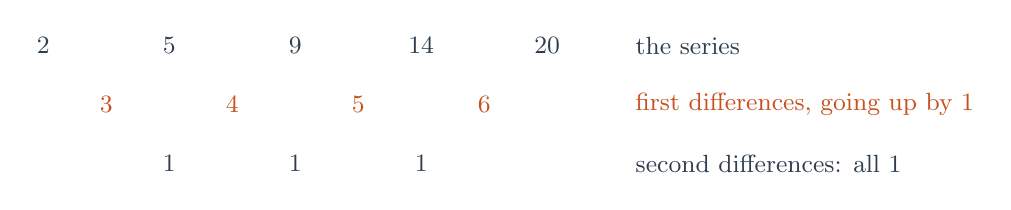
\begin{tikzpicture}[font=\small]
\foreach \xa/\val in {0/2,1.6/5,3.2/9,4.8/14,6.4/20}{\node[color=slate] at (\xa,0) {\val};}
\foreach \xa/\val in {0.8/3,2.4/4,4.0/5,5.6/6}{\node[color=ember] at (\xa,-0.75) {\val};}
\foreach \xa/\val in {1.6/1,3.2/1,4.8/1}{\node[color=slate] at (\xa,-1.5) {\val};}
\node[anchor=west,color=slate] at (7.4,0) {the series};
\node[anchor=west,color=ember] at (7.4,-0.75) {first differences, going up by 1};
\node[anchor=west,color=slate] at (7.4,-1.5) {second differences: all 1};
\end{tikzpicture}\par\nopagebreak\smallskip
{\small Since the second differences are all 1, the next first difference is 7, and the next term is $20 + 7 = 27$.}
\end{center}

\begin{center}\small\renewcommand{\arraystretch}{1.18}\setlength{\tabcolsep}{9pt}
\begin{tabularx}{\linewidth}{@{}c >{\raggedright\arraybackslash}X l@{}}
\toprule
\textbf{\color{slate}Step} & \textbf{\color{slate}Look for} & \textbf{\color{slate}Types} \\ \midrule
1 & the differences between neighbours & N1, N3, N4 \\
2 & the ratios between neighbours & N2, N6, N9 \\
3 & squares, cubes or primes nearby & N5, N8 \\
4 & a mixture: multiply then add, or sums of earlier terms & N6, N8 \\
5 & two series mixed together (alternate terms) & N7 \\
6 & letters instead of numbers & N12 \\
\bottomrule
\end{tabularx}\end{center}

\begin{center}\small\renewcommand{\arraystretch}{1.25}\setlength{\tabcolsep}{8pt}
\begin{tabularx}{\linewidth}{@{}l >{\raggedright\arraybackslash}X@{}}
\toprule
\textbf{\color{slate}Numbers to know} & \\ \midrule
Squares 1 to 15 & 1, 4, 9, 16, 25, 36, 49, 64, 81, 100, 121, 144, 169, 196, 225 \\
Cubes 1 to 10 & 1, 8, 27, 64, 125, 216, 343, 512, 729, 1000 \\
Primes up to 50 & 2, 3, 5, 7, 11, 13, 17, 19, 23, 29, 31, 37, 41, 43, 47 \\
\bottomrule
\end{tabularx}\end{center}

\infobox{Two habits that remove most mistakes}{
\begin{enumerate}
\item \textbf{Test the rule on every term}, not just the first two. Two terms fit many different rules.
\item \textbf{Write the differences under the series} before you think. Most rules show up there, or one row further down.
\end{enumerate}}

\subsection*{Spot-it table}
Read the series, find the row, jump to the type.
\begin{center}\small\renewcommand{\arraystretch}{1.18}\setlength{\tabcolsep}{7pt}
\begin{tabularx}{\linewidth}{@{}>{\raggedright\arraybackslash}X l >{\raggedright\arraybackslash}X@{}}
\toprule
\textbf{\color{slate}The series looks like} & \textbf{\color{slate}Type} & \textbf{\color{slate}The one move} \\ \midrule
7, 12, 17, 22, ? & N1 & the same difference each time \\
3, 6, 12, 24, ? & N2 & the same ratio each time \\
2, 5, 9, 14, 20, ? & N3 & the differences grow steadily \\
3, 4, 6, 10, 18, ? & N4 & the differences have their own pattern \\
2, 5, 10, 17, 26, ? & N5 & each term is near a square or a cube \\
3, 7, 15, 31, 63, ? & N6 & multiply, then add \\
2, 5, 4, 8, 6, 11, ? & N7 & split into two series \\
2, 3, 5, 7, 11, ?\ \ or \ 1, 2, 3, 5, 8, ? & N8 & primes, or sums of earlier terms \\
1, 1, 2, 6, 24, ? & N9 & growing multipliers, alternating steps \\
3, 7, 15, 31, 63, 128, 255 & N10 & find the wrong number \\
5, 8, ?, 14, 17 & N11 & find the missing term \\
A, C, F, J, ? & N12 & turn letters into positions \\
\bottomrule
\end{tabularx}\end{center}

\subsection{N1. Same difference each time}
\spot ``7, 12, 17, 22, ?'' ``45, 38, 31, 24, ?'' ``20th term of 4, 7, 10, 13, ...''

\mech
\begin{enumerate}
\item Subtract each term from the next. If it is always the same, that is the difference $d$.
\item Next term = last term + $d$. ($d$ is negative if the series goes down.)
\item The $n$th term $= a + (n - 1) \times d$, where $a$ is the first term.
\item Sum of $n$ terms $= \tfrac{n}{2} \times (\text{first} + \text{last})$.
\end{enumerate}

\samp 7, 12, 17, 22, ?
\begin{enumerate}
\item Differences: 5, 5, 5.
\item Next: $22 + 5 = 27$.
\end{enumerate}
\ans{27.}

\samp 45, 38, 31, 24, ?
\begin{enumerate}
\item Differences: $-7$ each time.
\item Next: $24 - 7 = 17$.
\end{enumerate}
\ans{17.}

\samp Find the 20th term of 4, 7, 10, 13, ... and the sum of the first 20 terms.
\begin{enumerate}
\item $a = 4$, $d = 3$.
\item 20th term: $4 + 19 \times 3 = 61$.
\item Sum: $\tfrac{20}{2} \times (4 + 61) = 10 \times 65 = 650$.
\end{enumerate}
\ans{61, and the sum is 650.}

\tryit (a) 11, 20, 29, 38, ? (b) The 100th term of 5, 9, 13, 17, ...

\subsection{N2. Same ratio each time}
\spot ``3, 6, 12, 24, ?'' ``5000, 1000, 200, 40, ?'' ``2, $-6$, 18, $-54$, ?''

\mech
\begin{enumerate}
\item Divide each term by the one before. If it is always the same, that is the ratio $r$.
\item $r$ can be a fraction (the series shrinks) or negative (signs switch).
\item Next term = last term $\times r$.
\item The $n$th term $= a \times r^{\,n-1}$.
\end{enumerate}

\samp 3, 6, 12, 24, ?
\begin{enumerate}
\item Ratio: 2.
\item Next: $24 \times 2 = 48$.
\end{enumerate}
\ans{48.}

\samp 5000, 1000, 200, 40, ?
\begin{enumerate}
\item Each term is the one before divided by 5.
\item Next: $40 \div 5 = 8$.
\end{enumerate}
\ans{8.}

\samp 2, $-6$, 18, $-54$, ?
\begin{enumerate}
\item Ratio: $-3$.
\item Next: $-54 \times (-3) = 162$.
\end{enumerate}
\ans{162.}

\samp Find the 8th term of 3, 6, 12, 24, ...
\begin{enumerate}
\item $3 \times 2^{7} = 3 \times 128 = 384$.
\end{enumerate}
\ans{384.}

\tryit (a) 2, 6, 18, 54, ? (b) 1458, 486, 162, 54, ? (c) The 7th term of 5, 10, 20, 40, ...

\subsection{N3. Differences that grow steadily}
\spot ``2, 5, 9, 14, 20, ?'' ``50, 44, 36, 26, 14, ?''

\mech
\begin{enumerate}
\item Write the differences. They are not all equal.
\item Write the differences of the differences. If they are all equal (call it $c$), the differences grow by $c$.
\item Next difference = last difference + $c$. Next term = last term + next difference.
\end{enumerate}

\samp 2, 5, 9, 14, 20, ?
\begin{enumerate}
\item Differences: 3, 4, 5, 6. They go up by 1.
\item Next difference: 7.
\item Next term: $20 + 7 = 27$.
\end{enumerate}
\ans{27.}

\samp 4, 5, 8, 13, 20, ?
\begin{enumerate}
\item Differences: 1, 3, 5, 7. They go up by 2.
\item Next difference: 9. Next term: $20 + 9 = 29$.
\end{enumerate}
\ans{29.}

\samp 50, 44, 36, 26, 14, ?
\begin{enumerate}
\item Differences: $-6, -8, -10, -12$. They go down by 2.
\item Next difference: $-14$. Next term: $14 - 14 = 0$.
\end{enumerate}
\ans{0.}

\tryit (a) 3, 4, 6, 9, 13, ? (b) 1, 4, 10, 19, 31, ?

\subsection{N4. Differences with a pattern of their own}
\spot ``3, 4, 6, 10, 18, ?'' ``1, 2, 6, 15, 31, ?'' ``1, 3, 6, 11, 18, 29, ?''

\mech
\begin{enumerate}
\item Write the differences.
\item Look at them as a new series. Common ones: doubling (1, 2, 4, 8), squares (1, 4, 9, 16), primes (2, 3, 5, 7, 11).
\item Continue that pattern, then add.
\end{enumerate}

\samp 3, 4, 6, 10, 18, ?
\begin{enumerate}
\item Differences: 1, 2, 4, 8. They double.
\item Next difference: 16. Next term: $18 + 16 = 34$.
\end{enumerate}
\ans{34.}

\samp 1, 2, 6, 15, 31, ?
\begin{enumerate}
\item Differences: 1, 4, 9, 16. Squares.
\item Next difference: 25. Next term: $31 + 25 = 56$.
\end{enumerate}
\ans{56.}

\samp 1, 3, 6, 11, 18, 29, ?
\begin{enumerate}
\item Differences: 2, 3, 5, 7, 11. Primes.
\item Next difference: 13. Next term: $29 + 13 = 42$.
\end{enumerate}
\ans{42.}

\tryit (a) 2, 3, 5, 9, 17, ? (b) 0, 1, 5, 14, 30, ?

\subsection{N5. Squares and cubes}
\spot ``2, 5, 10, 17, 26, ?'' ``2, 9, 28, 65, 126, ?'' ``2, 6, 12, 20, 30, ?''

\mech
\begin{enumerate}
\item Compare each term with the squares and cubes (table above).
\item Is each term the same amount above or below one? The rule is $n^2 \pm k$ or $n^3 \pm k$.
\item $n \times (n + 1)$ gives 2, 6, 12, 20, 30.
\end{enumerate}

\samp 2, 5, 10, 17, 26, ?
\begin{enumerate}
\item Each is 1 more than a square: $1 + 1$, $4 + 1$, $9 + 1$, $16 + 1$, $25 + 1$.
\item Next: $36 + 1 = 37$.
\end{enumerate}
\ans{37.}

\samp 0, 3, 8, 15, 24, ?
\begin{enumerate}
\item Each is 1 less than a square: $1 - 1$, $4 - 1$, $9 - 1$, ...
\item Next: $36 - 1 = 35$.
\end{enumerate}
\ans{35.}

\samp 2, 9, 28, 65, 126, ?
\begin{enumerate}
\item Each is 1 more than a cube: $1 + 1$, $8 + 1$, $27 + 1$, $64 + 1$, $125 + 1$.
\item Next: $216 + 1 = 217$.
\end{enumerate}
\ans{217.}

\samp 2, 6, 12, 20, 30, ?
\begin{enumerate}
\item $1 \times 2$, $2 \times 3$, $3 \times 4$, $4 \times 5$, $5 \times 6$.
\item Next: $6 \times 7 = 42$.
\end{enumerate}
\ans{42.}

\tryit (a) 3, 8, 15, 24, 35, ? (b) 0, 7, 26, 63, 124, ?

\subsection{N6. Multiply, then add}
\spot ``3, 7, 15, 31, 63, ?'' ``2, 5, 14, 41, 122, ?'' ``4, 9, 20, 43, ?''

\mech
\begin{enumerate}
\item The terms grow fast, but the ratio is not the same each time.
\item Write the differences. If they double, multiply by 2. If they triple, multiply by 3.
\item Find what is added each time: term $\times a \pm b$ = next term.
\item If the added number grows by 1 each step (+1, +2, +3), the rule is $\times a + 1, +2, +3, \dots$
\end{enumerate}

\samp 3, 7, 15, 31, 63, ?
\begin{enumerate}
\item Differences: 4, 8, 16, 32. They double, so $\times 2$.
\item $3 \times 2 + 1 = 7$, $7 \times 2 + 1 = 15$. The rule is $\times 2 + 1$.
\item Next: $63 \times 2 + 1 = 127$.
\end{enumerate}
\ans{127.}

\samp 2, 5, 14, 41, 122, ?
\begin{enumerate}
\item Differences: 3, 9, 27, 81. They triple, so $\times 3$.
\item $2 \times 3 - 1 = 5$. The rule is $\times 3 - 1$.
\item Next: $122 \times 3 - 1 = 365$.
\end{enumerate}
\ans{365.}

\samp 4, 9, 20, 43, ?
\begin{enumerate}
\item $4 \times 2 + 1 = 9$, $9 \times 2 + 2 = 20$, $20 \times 2 + 3 = 43$.
\item Next: $43 \times 2 + 4 = 90$.
\end{enumerate}
\ans{90.}

\tryit (a) 5, 11, 23, 47, 95, ? (b) 1, 4, 13, 40, ?

\subsection{N7. Two series mixed together}
\spot ``2, 5, 4, 8, 6, 11, 8, ?'' ``3, 10, 6, 20, 12, 40, ?''

\mech
\begin{enumerate}
\item If no single rule fits, split the series in two.
\item Odd positions: 1st, 3rd, 5th, ... Even positions: 2nd, 4th, 6th, ...
\item Each part is usually a simple series.
\item The missing term belongs to whichever part its position is in.
\end{enumerate}

\samp 2, 5, 4, 8, 6, 11, 8, ?
\begin{enumerate}
\item Odd positions: 2, 4, 6, 8.
\item Even positions: 5, 8, 11, and next 14.
\item The missing term is the 8th, an even position.
\end{enumerate}
\ans{14.}

\samp 3, 10, 6, 20, 12, 40, ?
\begin{enumerate}
\item Odd positions: 3, 6, 12 (doubling).
\item Even positions: 10, 20, 40 (doubling).
\item The 7th term is an odd position: $12 \times 2 = 24$.
\end{enumerate}
\ans{24.}

\samp 100, 5, 90, 10, 80, 15, ?
\begin{enumerate}
\item Odd positions: 100, 90, 80 (down 10).
\item Even positions: 5, 10, 15 (up 5).
\item The 7th term is an odd position: $80 - 10 = 70$.
\end{enumerate}
\ans{70.}

\tryit (a) 1, 20, 3, 17, 5, 14, 7, ? (b) 8, 3, 16, 6, 32, 9, ?

\subsection{N8. Primes and sums of earlier terms}
\spot ``2, 3, 5, 7, 11, 13, ?'' ``3, 4, 6, 8, 12, 14, ?'' ``1, 2, 3, 5, 8, 13, ?''

\mech
\begin{enumerate}
\item \textbf{Primes:} 2, 3, 5, 7, 11, 13, 17, 19, 23, ... The series may be the primes, or primes $\pm$ a number.
\item \textbf{Fibonacci type:} each term = the two before added. Variants: add a number as well, or add the \emph{three} before.
\end{enumerate}

\samp 3, 4, 6, 8, 12, 14, ?
\begin{enumerate}
\item These are the primes plus 1: $2 + 1$, $3 + 1$, $5 + 1$, $7 + 1$, $11 + 1$, $13 + 1$.
\item Next prime is 17. Next term: $17 + 1 = 18$.
\end{enumerate}
\ans{18.}

\samp 1, 2, 3, 5, 8, 13, ?
\begin{enumerate}
\item $1 + 2 = 3$, $2 + 3 = 5$, $3 + 5 = 8$, $5 + 8 = 13$.
\item Next: $8 + 13 = 21$.
\end{enumerate}
\ans{21.}

\samp 2, 3, 6, 10, 17, 28, ?
\begin{enumerate}
\item Two before, plus 1: $2 + 3 + 1 = 6$, $3 + 6 + 1 = 10$, $6 + 10 + 1 = 17$.
\item Next: $17 + 28 + 1 = 46$.
\end{enumerate}
\ans{46.}

\samp 1, 2, 4, 7, 13, 24, ?
\begin{enumerate}
\item Three before: $1 + 2 + 4 = 7$, $2 + 4 + 7 = 13$, $4 + 7 + 13 = 24$.
\item Next: $7 + 13 + 24 = 44$.
\end{enumerate}
\ans{44.}

\tryit (a) 4, 5, 7, 9, 13, ? (b) 4, 6, 10, 16, 26, ? (c) 1, 1, 3, 5, 9, 17, ?

\subsection{N9. Growing multipliers and switching steps}
\spot ``1, 1, 2, 6, 24, 120, ?'' ``5, 10, 8, 16, 14, 28, ?''

\mech
\begin{enumerate}
\item \textbf{Growing multipliers:} divide each term by the one before. If you get 1, 2, 3, 4, ..., the next multiplier is one more.
\item \textbf{Switching steps:} the rule changes every step, for example $\times 2$, then $-2$, then $\times 2$ again. Look at the steps in pairs.
\end{enumerate}

\samp 1, 1, 2, 6, 24, 120, ?
\begin{enumerate}
\item Multipliers: $\times 1$, $\times 2$, $\times 3$, $\times 4$, $\times 5$.
\item Next: $\times 6$. $120 \times 6 = 720$.
\end{enumerate}
\ans{720.}

\samp 2, 4, 12, 48, 240, ?
\begin{enumerate}
\item Multipliers: $\times 2$, $\times 3$, $\times 4$, $\times 5$.
\item Next: $\times 6$. $240 \times 6 = 1440$.
\end{enumerate}
\ans{1440.}

\samp 5, 10, 8, 16, 14, 28, ?
\begin{enumerate}
\item Steps: $\times 2$, $-2$, $\times 2$, $-2$, $\times 2$.
\item Next step: $-2$. $28 - 2 = 26$.
\end{enumerate}
\ans{26.}

\tryit (a) 3, 6, 18, 72, 360, ? (b) 4, 8, 6, 12, 10, 20, ?

\subsection{N10. Find the wrong number}
\spot ``Find the wrong number: 3, 7, 15, 31, 63, 128, 255.''

\mech
\begin{enumerate}
\item Find the rule from the first few terms.
\item Run the rule along the series. The first term that does not fit is the suspect.
\item Replace it with the right value. Check that the terms after it still fit.
\end{enumerate}

\samp Find the wrong number: 3, 7, 15, 31, 63, 128, 255.
\begin{enumerate}
\item Rule from the start: $\times 2 + 1$.
\item After 63 should come $63 \times 2 + 1 = 127$, not 128.
\item Check: $127 \times 2 + 1 = 255$, which fits.
\end{enumerate}
\ans{128 (it should be 127).}

\samp Find the wrong number: 2, 5, 10, 17, 26, 36, 50.
\begin{enumerate}
\item Rule: square + 1.
\item The 6th term should be $36 + 1 = 37$.
\end{enumerate}
\ans{36 (it should be 37).}

\samp Find the wrong number: 4, 8, 16, 32, 62, 128.
\begin{enumerate}
\item Rule: doubling. After 32 comes 64.
\item Check: $64 \times 2 = 128$, which fits.
\end{enumerate}
\ans{62 (it should be 64).}

\tryit Find the wrong number. (a) 5, 11, 23, 47, 96, 191. (b) 1, 4, 9, 16, 26, 36, 49.

\subsection{N11. Find the missing term}
\spot ``5, 8, ?, 14, 17'' ``2, ?, 10, 17, ?, 37''

\mech
\begin{enumerate}
\item Use the terms on \emph{both} sides of the gap. The rule must fit all of them.
\item Across one gap, the two neighbours are two steps apart. Halve their difference for a same-difference series.
\item With two gaps, find the rule from the terms you have, fill in, and check.
\end{enumerate}

\samp 5, 8, ?, 14, 17
\begin{enumerate}
\item $5 \to 8$ is $+3$, and $14 \to 17$ is $+3$.
\item The gap: $8 + 3 = 11$.
\item Check: 8 to 14 is 6, two steps of 3.
\end{enumerate}
\ans{11.}

\samp 2, 6, ?, 54, 162
\begin{enumerate}
\item $2 \to 6$ is $\times 3$, and $54 \to 162$ is $\times 3$.
\item The gap: $6 \times 3 = 18$.
\end{enumerate}
\ans{18.}

\samp 2, ?, 10, 17, ?, 37
\begin{enumerate}
\item 10, 17 and 37 are $9 + 1$, $16 + 1$ and $36 + 1$. The rule is square + 1.
\item The gaps: $4 + 1 = 5$ and $25 + 1 = 26$.
\end{enumerate}
\ans{5 and 26.}

\tryit (a) 6, 13, ?, 27, 34 (b) 2, ?, 14, 30, 62

\subsection{N12. Letter series}
\spot ``A, C, F, J, O, ?'' ``Z, X, U, Q, L, ?''

\mech
\begin{enumerate}
\item Replace each letter by its place in the alphabet (table below).
\item Find the rule on the numbers, as in N1 to N9.
\item Turn the answer back into a letter. After 26 (Z), go round: 27 is A.
\end{enumerate}

\subsection*{Shortcuts to memorise}
\begin{center}\small\renewcommand{\arraystretch}{1.9}\setlength{\tabcolsep}{8pt}
\begin{tabularx}{\linewidth}{@{}>{\raggedright\arraybackslash}X>{\raggedright\arraybackslash}X@{}}
\toprule
\textbf{\color{slate}Idea} & \textbf{\color{slate}Rule} \\ \midrule
Constant difference & $n$th term $=a+(n-1)d$ \\
Constant ratio & $n$th term $=a\,r^{\,n-1}$ \\
Differences grow by $c$ & the next difference is the last plus $c$ \\
Differences double, square, prime & extend the pattern, then add \\
Near a square or cube & $n^2\pm k$, $n^3\pm k$, $n(n+1)$ \\
Differences double or triple & the rule is $\times 2\pm b$ or $\times 3\pm b$ \\
Mixed series & split into odd and even positions \\
Fibonacci type & sum of the two (or three) before \\
Ratios 1, 2, 3, ... & factorial-type growth \\
Wrong number & run the rule, find the first misfit, check the rest \\
Letters & position 1 to 26, wrap round after Z \\
\bottomrule
\end{tabularx}\end{center}

\subsection*{Sanity checks before you mark the option}
\infobox{Ten seconds that save a wrong answer}{
\begin{itemize}
\item Does your rule produce \emph{every} given term, not just the first two?
\item Is the size of the answer sensible? A series that doubles will not suddenly go up by 3.
\item For ``find the wrong number'', do the terms after your corrected number still follow the rule?
\item For letter series, did you go round after Z?
\item If two rules fit, take the simpler one that fits all the terms.
\end{itemize}}

\subsection*{Traps}
\begin{enumerate}
\item \textbf{Looking only at differences when the pattern is in the ratios} (N2, N6), or the other way round.
\item \textbf{Stopping at the first rule that fits two terms.} Test it on all of them.
\item \textbf{Missing that the series is two series mixed} (N7).
\item \textbf{The wrong sign in a falling series} (N1, N3). Down by 7 is $-7$.
\item \textbf{A square used where the term is near a cube}, or $n^2+1$ read as $(n+1)^2$ (N5).
\item \textbf{Forgetting the changing number in $\times a + n$} (N6).
\item \textbf{Counting positions wrongly in a mixed series} (N7). The 7th term is an odd position.
\item \textbf{Calling 1 or 9 a prime} (N8). 1 is not prime, and 9 is $3\times3$.
\item \textbf{Naming the wrong number without checking the later terms} (N10).
\item \textbf{Not going round after Z} (N12).
\end{enumerate}

\subsection*{Answers to ``Try it''}
\begin{center}\small\renewcommand{\arraystretch}{1.25}\setlength{\tabcolsep}{8pt}
\begin{tabularx}{\linewidth}{@{}l>{\raggedright\arraybackslash}p{3.4cm}>{\raggedright\arraybackslash}X@{}}
\toprule
\textbf{\color{slate}Type} & \textbf{\color{slate}Answer} & \textbf{\color{slate}Working, step by step} \\ \midrule
N1 & (a) 47 \newline (b) 401 & (a) Step 9. $38 + 9$. \newline (b) $5 + 99 \times 4$. \\
N2 & (a) 162 \newline (b) 18 \newline (c) 320 & (a) $\times 3$. \newline (b) $\div 3$. \newline (c) $5 \times 2^6 = 5 \times 64$. \\
N3 & (a) 18 \newline (b) 46 & (a) Differences 1, 2, 3, 4, then 5. \newline (b) Differences 3, 6, 9, 12, then 15. \\
N4 & (a) 33 \newline (b) 55 & (a) Differences 1, 2, 4, 8, then 16. \newline (b) Differences 1, 4, 9, 16 (squares), then 25. \\
N5 & (a) 48 \newline (b) 215 & (a) Squares from 4, minus 1: next $49 - 1$. \newline (b) Cubes minus 1: next $216 - 1$. \\
N6 & (a) 191 \newline (b) 121 & (a) $\times 2 + 1$. \newline (b) $\times 3 + 1$. \\
N7 & (a) 11 \newline (b) 64 & (a) Even positions 20, 17, 14, then 11. \newline (b) Odd positions double: 8, 16, 32, 64. \\
N8 & (a) 15 \newline (b) 42 \newline (c) 31 & (a) Primes + 2. Next prime 13. \newline (b) Two before: $16 + 26$. \newline (c) Three before: $5 + 9 + 17$. \\
N9 & (a) 2160 \newline (b) 18 & (a) $\times 2, \times 3, \times 4, \times 5$, then $\times 6$. \newline (b) $\times 2$ and $-2$ in turn. \\
N10 & (a) 96, should be 95 \newline (b) 26, should be 25 & (a) $\times 2 + 1$. \newline (b) Squares. \\
N11 & (a) 20 \newline (b) 6 & (a) Step 7. \newline (b) $\times 2 + 2$. \\
N12 & (a) R \newline (b) S & (a) Places 3, 6, 9, 12, 15, then 18. \newline (b) Places 4, 5, 7, 10, 14. Differences 1, 2, 3, 4, then 5: 19. \\
\bottomrule
\end{tabularx}\end{center}

\clearpage
\keepsamptrue
\section[Syllogisms (Y1--Y12)]{Syllogisms (with Venn diagrams)}\label{ch:Y}
\addtocontents{toc}{\protect\nopagebreak}

\subsection*{The one idea}
A syllogism gives you statements about groups (all, no, some) and asks what \emph{must} follow. Draw each statement as circles. A conclusion \textbf{follows} only if it is true in \emph{every} picture the statements allow. If you can draw one allowed picture where it is false, it does not follow. Use only the statements, never what you know about the world.

\begin{center}
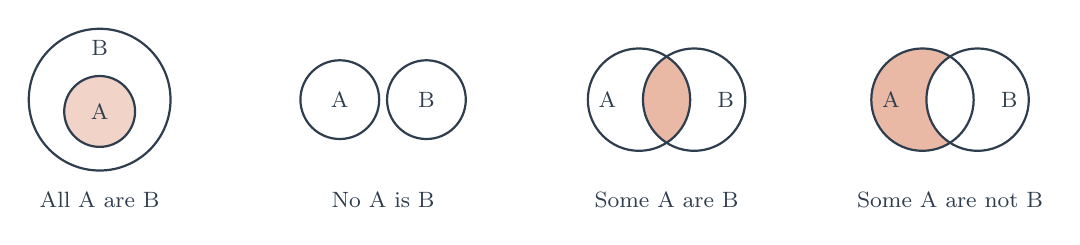
\begin{tikzpicture}[font=\footnotesize]
\begin{scope}
\draw[color=slate,thick] (0,0) circle (0.9);
\draw[color=slate,thick,fill=ember!25] (0,-0.15) circle (0.45);
\node[color=slate] at (0,-0.15) {A};
\node[color=slate] at (0,0.66) {B};
\node[anchor=north,color=slate] at (0,-1.05) {All A are B};
\end{scope}
\begin{scope}[xshift=3.6cm]
\draw[color=slate,thick] (-0.55,0) circle (0.5);
\draw[color=slate,thick] (0.55,0) circle (0.5);
\node[color=slate] at (-0.55,0) {A};
\node[color=slate] at (0.55,0) {B};
\node[anchor=north,color=slate] at (0,-1.05) {No A is B};
\end{scope}
\begin{scope}[xshift=7.2cm]
\begin{scope}
\clip (-0.35,0) circle (0.65);
\fill[ember!40] (0.35,0) circle (0.65);
\end{scope}
\draw[color=slate,thick] (-0.35,0) circle (0.65);
\draw[color=slate,thick] (0.35,0) circle (0.65);
\node[color=slate] at (-0.75,0) {A};
\node[color=slate] at (0.75,0) {B};
\node[anchor=north,color=slate] at (0,-1.05) {Some A are B};
\end{scope}
\begin{scope}[xshift=10.8cm]
\fill[ember!40] (-0.35,0) circle (0.65);
\fill[white] (0.35,0) circle (0.65);
\draw[color=slate,thick] (-0.35,0) circle (0.65);
\draw[color=slate,thick] (0.35,0) circle (0.65);
\node[color=slate] at (-0.75,0) {A};
\node[color=slate] at (0.75,0) {B};
\node[anchor=north,color=slate] at (0,-1.05) {Some A are not B};
\end{scope}
\end{tikzpicture}\par\nopagebreak\smallskip
{\small The four statements as pictures. The shaded part is where at least one member must be.}
\end{center}

\infobox{Two habits that remove most mistakes}{
\begin{enumerate}
\item \textbf{Try to break the conclusion with a picture.} If any allowed picture makes it false, it does not follow.
\item \textbf{Use only the statements.} Ignore real-world facts. ``All cats are animals'' counts only if a statement says it.
\end{enumerate}}

\subsection*{Spot-it table}
Read the wording, find the row, jump to the type.
\begin{center}\small\renewcommand{\arraystretch}{1.18}\setlength{\tabcolsep}{7pt}
\begin{tabularx}{\linewidth}{@{}>{\raggedright\arraybackslash}X l >{\raggedright\arraybackslash}X@{}}
\toprule
\textbf{\color{slate}Wording in the question} & \textbf{\color{slate}Type} & \textbf{\color{slate}The one move} \\ \midrule
``All cats are animals'': what else is true & Y1 & draw the picture \\
Does ``Some B are A'' follow from ``Some A are B'' & Y2 & which statements flip \\
All A are B, all B are C & Y3 & a chain of ``all'' \\
All books are papers, no paper is a stone & Y4 & look up the eight pairs \\
Some pens are books, some books are bags & Y5 & nothing follows \\
Must the conclusion always be true & Y6 & try to make it fail \\
``Either I or II follows'' & Y7 & a complementary pair \\
Three statements in a row & Y8 & combine two at a time \\
``Only doctors are surgeons'' & Y9 & translate the wording \\
``Some cats can be birds'' & Y10 & can any picture make it true \\
In a class of 60, 35 play cricket, 28 football & Y11 & add, then take away the overlap \\
Which diagram shows lions, tigers, animals & Y12 & compare the terms in pairs \\
\bottomrule
\end{tabularx}\end{center}

\subsection{Y1. The four statements and what each tells you}
\spot ``All cats are animals.'' ``No pen is a book.'' ``Some doctors are teachers.'' ``Some men are not students.''

\mech
\begin{enumerate}
\item Four forms: \textbf{All} A are B, \textbf{No} A is B, \textbf{Some} A are B, \textbf{Some} A are \textbf{not} B (the pictures above).
\item ``Some'' means \emph{at least one}, and possibly all of them.
\item In these questions every group named has members. So ``All A are B'' also gives ``Some A are B'', and ``No A is B'' also gives ``Some A are not B''.
\end{enumerate}

\begin{center}\small\renewcommand{\arraystretch}{1.18}\setlength{\tabcolsep}{8pt}
\begin{tabularx}{\linewidth}{@{}l >{\raggedright\arraybackslash}X >{\raggedright\arraybackslash}X@{}}
\toprule
\textbf{\color{slate}Statement} & \textbf{\color{slate}Also follows} & \textbf{\color{slate}Does not follow} \\ \midrule
All A are B & Some A are B; Some B are A & All B are A \\
No A is B & No B is A; Some A are not B; Some B are not A & Some A are B \\
Some A are B & Some B are A & All A are B; Some A are not B \\
Some A are not B & nothing more about A and B & Some B are not A; No A is B \\
\bottomrule
\end{tabularx}\end{center}

\samp All cats are animals.
\begin{enumerate}
\item ``Some cats are animals'': \textbf{follows}.
\item ``All animals are cats'': \textbf{does not follow} (the animal circle can be bigger).
\end{enumerate}
\samp No pen is a book.
\begin{enumerate}
\item ``No book is a pen'': \textbf{follows}.
\item ``Some books are not pens'': \textbf{follows}.
\item ``Some pens are books'': \textbf{does not follow}.
\end{enumerate}
\samp Some doctors are teachers.
\begin{enumerate}
\item ``Some teachers are doctors'': \textbf{follows}.
\item ``All doctors are teachers'' and ``Some doctors are not teachers'': \textbf{neither follows}.
\end{enumerate}
\samp Some men are not students.
\begin{enumerate}
\item ``Some students are not men'': \textbf{does not follow}.
\item ``No man is a student'': \textbf{does not follow}.
\end{enumerate}

\tryit (a) ``No dog is a cat.'' Does ``Some cats are not dogs'' follow? (b) ``Some players are not doctors.'' Does ``Some doctors are not players'' follow?

\subsection{Y2. Converting a statement}
\spot ``All students are boys. Does it follow that all boys are students?''

\mech Which statements can be turned round (subject and predicate swapped)?
\begin{center}\small\renewcommand{\arraystretch}{1.18}\setlength{\tabcolsep}{9pt}
\begin{tabular}{@{}lll@{}}
\toprule
\textbf{\color{slate}Statement} & \textbf{\color{slate}Turn it round?} & \textbf{\color{slate}Result} \\ \midrule
Some A are B & yes & Some B are A \\
No A is B & yes & No B is A \\
All A are B & only partly & Some B are A (not All B are A) \\
Some A are not B & no & nothing \\
\bottomrule
\end{tabular}\end{center}

\samp All students are boys.
\begin{enumerate}
\item ``Some boys are students'': \textbf{follows}.
\item ``All boys are students'': \textbf{does not follow}.
\end{enumerate}
\samp No book is a pen. ``No pen is a book'': \textbf{follows}.

\samp Some men are not women. ``Some women are not men'': \textbf{does not follow}.

\tryit (a) ``Some chairs are tables.'' Does ``Some tables are chairs'' follow? (b) ``All roses are flowers.'' Does ``All flowers are roses'' follow? Does ``Some flowers are roses''?

\subsection{Y3. All and all: a chain}
\spot ``All pens are books. All books are papers. I. All pens are papers. II. All papers are pens.''

\mech
\begin{enumerate}
\item Put the statements in a chain so the middle term links them: A $\to$ B, B $\to$ C.
\item All A are B and all B are C: \textbf{All A are C} follows. So does ``Some C are A'' (the partial flip).
\item ``All C are A'' does \emph{not} follow. The C circle may be bigger.
\end{enumerate}

\samp All pens are books. All books are papers.
\begin{enumerate}
\item I.
\item All pens are papers: \textbf{follows}.
\item II.
\item All papers are pens: \textbf{does not follow}.
\item ``Some papers are pens'': \textbf{follows}.
\end{enumerate}
\samp All teachers are graduates. All graduates are readers. I. All readers are graduates. II. Only some teachers are readers.
\begin{enumerate}
\item I does not follow (the reader circle can be bigger).
\item II would mean some teachers are \emph{not} readers, but all of them are. \textbf{Neither follows.}
\end{enumerate}

\tryit All dogs are animals. All animals are living things. I. All dogs are living things. II. All living things are animals. Which follow?

\subsection{Y4. The eight pairs that give a conclusion}
\spot ``All books are papers. No paper is a stone. Conclusion: No book is a stone.''

\mech
\begin{enumerate}
\item Find the \textbf{middle term}: the term that appears in both statements (B below).
\item Line the statements up so B is last in the first and first in the second: A--B, then B--C. Turn a statement round only as Y2 allows: Some and No turn round freely, All turns into Some.
\item Read the conclusion from the table. A pair that is not in the table gives nothing (Y5).
\end{enumerate}
\begin{center}\small\renewcommand{\arraystretch}{1.18}\setlength{\tabcolsep}{9pt}
\begin{tabular}{@{}rlll@{}}
\toprule
 & \textbf{\color{slate}First} & \textbf{\color{slate}Second} & \textbf{\color{slate}Conclusion} \\ \midrule
1 & All A are B & All B are C & All A are C \\
2 & All A are B & No B is C & No A is C \\
3 & Some A are B & All B are C & Some A are C \\
4 & Some A are B & No B is C & Some A are not C \\
5 & No A is B & All B are C & Some C are not A \\
6 & No A is B & Some B are C & Some C are not A \\
7 & All A are B & Some C are not B & Some C are not A \\
8 & Some B are not A & All B are C & Some C are not A \\
\bottomrule
\end{tabular}\end{center}
Rows 5 to 8 all end in ``Some C are not A''. Rows 7 and 8 cannot be lined up (a ``Some are not'' statement never turns round), so learn them as they stand: in row 7 the middle term B is last in both statements, in row 8 it is first in both.

\samp All books are papers. No paper is a stone.
\begin{enumerate}
\item All + No gives \textbf{No book is a stone}.
\item It follows.
\end{enumerate}
\samp Some doctors are men. All men are mortal.
\begin{enumerate}
\item Some + All gives \textbf{Some doctors are mortal}.
\item It follows.
\end{enumerate}
\samp Some rivers are lakes. No lake is a hill.
\begin{enumerate}
\item Some + No gives \textbf{Some rivers are not hills}.
\item It follows.
\end{enumerate}
\samp No cat is a bird. All birds are flyers.
\begin{enumerate}
\item No + All gives \textbf{Some flyers are not cats}.
\item It follows.
\item ``No cat is a flyer'' \textbf{does not follow}.
\end{enumerate}
\samp All pens are books. Some cups are not books.
\begin{enumerate}
\item Row 7.
\item A cup outside the books cannot be a pen (every pen is a book), so \textbf{Some cups are not pens}.
\item ``Some pens are not cups'': \textbf{does not follow}.
\end{enumerate}
\samp Some pens are not cups. All pens are books.
\begin{enumerate}
\item Row 8.
\item Those pens are books too, so \textbf{Some books are not cups}.
\end{enumerate}

\tryit (a) Some pens are ink. All ink is liquid. Does ``Some pens are liquid'' follow? (b) No fish is a bird. Some birds are swimmers. Does ``Some swimmers are not fish'' follow? (c) All lions are animals. Some tigers are not animals. Does ``Some tigers are not lions'' follow?

\subsection{Y5. When nothing follows}
\spot ``Some pens are books. Some books are bags. Conclusion: Some pens are bags.''

\mech If the pair is not one of the eight rows of Y4 (after the allowed turn-rounds), \textbf{nothing follows}. Three quick checks rule out most pairs:
\begin{enumerate}
\item Both statements are ``some'' type (Some, or Some are not): nothing follows.
\item Both statements are negative (No, or Some are not): nothing follows.
\item The middle term is never \textbf{covered}: nothing follows. B is covered when it is the first term of an ``All'' (All B are \dots), is in a ``No'', or comes after ``not'' in a ``Some are not''. If it is only the second term of an ``All'' or sits inside a ``Some'', nothing ties the two statements together.
\end{enumerate}
A pair can pass all three checks and still give nothing (the last sample), so the table has the final word.

\samp All birds are animals. Some animals are fliers.
\begin{enumerate}
\item ``Animals'' is only the big side of an ``All'' and sits inside a ``Some'': not covered.
\item ``Some birds are fliers'', ``All birds are fliers'' and ``Some fliers are birds'': \textbf{none follows}.
\end{enumerate}
\samp Some pens are books. Some books are bags.
\begin{enumerate}
\item Two ``some'' statements.
\item ``Some pens are bags'': \textbf{does not follow}.
\end{enumerate}
\samp No tree is a rock. No rock is a river.
\begin{enumerate}
\item Two negatives.
\item ``No tree is a river'' and ``Some trees are rivers'': \textbf{neither follows}.
\end{enumerate}
\samp Some men are not doctors. All doctors are lawyers.
\begin{enumerate}
\item It looks like a chain and passes all three checks, but it is not in the table.
\item ``Some men are not lawyers'': \textbf{does not follow} (the men who are not doctors may all be lawyers).
\end{enumerate}

\tryit (a) All cats are dogs. All birds are dogs. Does ``All cats are birds'' follow? (b) Some A are not B. No B is C. Does ``Some A are not C'' follow?

\subsection{Y6. Test a conclusion: can a picture make it fail?}
\spot ``All A are B. Some B are C. Conclusion: Some A are C.''

\mech
\begin{enumerate}
\item Draw the statements the loosest way they allow.
\item Try to draw an allowed picture where the conclusion is \emph{false}.
\item If you can, it does not follow. If every allowed picture makes it true, it follows.
\end{enumerate}

\begin{center}
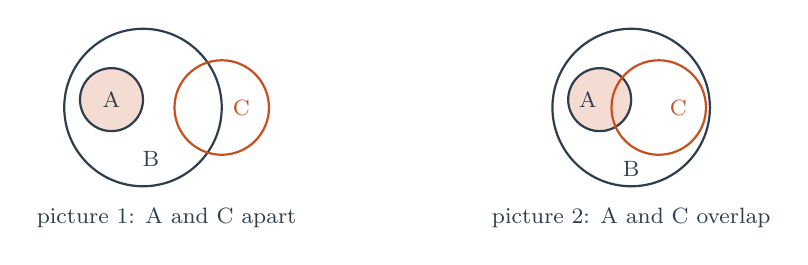
\begin{tikzpicture}[font=\footnotesize]
\begin{scope}
\draw[color=slate,thick] (0,0) circle (1.0);
\draw[color=slate,thick,fill=ember!20] (-0.4,0.1) circle (0.4);
\draw[color=ember,thick] (1.0,0) circle (0.6);
\node[color=slate] at (-0.4,0.1) {A};
\node[color=slate] at (0.1,-0.65) {B};
\node[color=ember] at (1.25,0) {C};
\node[anchor=north,color=slate] at (0.3,-1.15) {picture 1: A and C apart};
\end{scope}
\begin{scope}[xshift=6.2cm]
\draw[color=slate,thick] (0,0) circle (1.0);
\draw[color=slate,thick,fill=ember!20] (-0.4,0.1) circle (0.4);
\draw[color=ember,thick] (0.35,0) circle (0.6);
\node[color=slate] at (-0.55,0.1) {A};
\node[color=slate] at (0,-0.78) {B};
\node[color=ember] at (0.6,0) {C};
\node[anchor=north,color=slate] at (0,-1.15) {picture 2: A and C overlap};
\end{scope}
\end{tikzpicture}\par\nopagebreak\smallskip
{\small Both pictures obey ``All A are B'' and ``Some B are C''. ``Some A are C'' is false in picture 1, so it does not follow.}
\end{center}

\samp All A are B. Some B are C.
\begin{enumerate}
\item ``Some A are C'': \textbf{does not follow} (picture 1).
\item ``Some C are B'': \textbf{follows} (it is just ``Some B are C'' turned round).
\end{enumerate}
\samp Some A are B. No B is C.
\begin{enumerate}
\item ``No A is C'': \textbf{does not follow} (the A that are not B may be C).
\item ``Some A are not C'': \textbf{follows} (Y4).
\end{enumerate}
\samp All pens are books. Some books are cups.
\begin{enumerate}
\item ``Some pens are not cups'': \textbf{does not follow}.
\item All the pens could sit inside the cups.
\end{enumerate}

\tryit (a) All A are B. Some A are C. Does ``Some B are C'' follow? (b) All A are B. Some C are B. Does ``Some C are A'' follow?

\subsection{Y7. Either--or}
\spot ``All pens are books. Some books are cups. I. Some pens are cups. II. No pen is a cup.''

\mech
\begin{enumerate}
\item Check each conclusion on its own first. If one follows, either--or does not apply.
\item If neither follows, look at the pair. Both must be about the \emph{same two terms} and form one of these pairs:
\end{enumerate}
\begin{center}\small\renewcommand{\arraystretch}{1.18}\setlength{\tabcolsep}{9pt}
\begin{tabular}{@{}ll@{}}
\toprule
\textbf{\color{slate}Pair} & \textbf{\color{slate}Why it works} \\ \midrule
Some A are B $/$ No A is B & exactly one is true \\
All A are B $/$ Some A are not B & exactly one is true \\
Some A are B $/$ Some A are not B & at least one is true \\
\bottomrule
\end{tabular}\end{center}
\begin{enumerate}
\setcounter{enumi}{2}
\item Then the answer is \textbf{either I or II follows}. ``All A are B'' with ``No A is B'' is \emph{not} such a pair: both can be false.
\end{enumerate}

\samp All pens are books. Some books are cups. I. Some pens are cups. II. No pen is a cup.
\begin{enumerate}
\item Neither follows alone (the pens may or may not touch the cups).
\item The pair is Some / No, so \textbf{either I or II follows}.
\end{enumerate}
\samp All cats are dogs. Some dogs are birds. I. All cats are birds. II. Some cats are not birds.
\begin{enumerate}
\item Neither alone.
\item The pair is All / Some not, so \textbf{either I or II}.
\end{enumerate}
\samp Same pens and cups. I. All pens are cups. II. No pen is a cup.
\begin{enumerate}
\item Neither follows, and All / No is not a complementary pair (both are false if some pens are cups and some are not).
\item The answer is \textbf{neither}.
\end{enumerate}

\tryit Some A are B. Some B are C. I. Some A are C. II. No A is C. What follows?

\subsection{Y8. Three statements}
\spot ``All A are B. All B are C. All C are D. Conclusion: All A are D.''

\mech Combine the first two with the Y4 table, then combine the result with the third. Each step must connect through a shared term.

\samp All A are B. All B are C. All C are D.
\begin{enumerate}
\item All + All gives All A are C.
\item Then All A are C and All C are D give \textbf{All A are D}.
\item ``Some D are A'' also follows.
\end{enumerate}
\samp Some A are B. All B are C. No C is D.
\begin{enumerate}
\item Some + All gives Some A are C.
\item Then Some A are C and No C is D (Some + No) give \textbf{Some A are not D}.
\end{enumerate}
\samp All A are B. No B is C. Some C are D.
\begin{enumerate}
\item All + No gives No A is C.
\item Then No A is C and Some C are D (No + Some) give \textbf{Some D are not A}.
\end{enumerate}

\tryit (a) Some P are Q. All Q are R. All R are S. Does ``Some P are S'' follow? (b) All X are Y. Some Y are Z. All Z are W. Does ``Some Y are W'' follow? Does ``Some X are W''?

\subsection{Y9. Reading the wording}
\spot ``Only doctors are surgeons.'' ``Only some pens are red.'' ``Not all birds are crows.''

\mech
\begin{center}\small\renewcommand{\arraystretch}{1.18}\setlength{\tabcolsep}{9pt}
\begin{tabularx}{\linewidth}{@{}>{\raggedright\arraybackslash}X >{\raggedright\arraybackslash}X@{}}
\toprule
\textbf{\color{slate}Wording} & \textbf{\color{slate}Means} \\ \midrule
Every, each, any A is B & All A are B \\
None of the A is B; A is never B & No A is B \\
Some, several A are B & Some A are B \\
\textbf{Only} A are B & \textbf{All B are A} (it flips) \\
Only some A are B & Some A are B \emph{and} some A are not B \\
Not all A are B & Some A are not B \\
\bottomrule
\end{tabularx}\end{center}
Books differ on ``few'': some treat ``Few A are B'' as ``Some A are B'', others as ``only some''. Check one solved example in your book and follow it.

\samp Only doctors are surgeons.
\begin{enumerate}
\item That is ``All surgeons are doctors''.
\item So ``Some doctors are surgeons'': \textbf{follows}.
\item ``All doctors are surgeons'': \textbf{does not follow}.
\end{enumerate}
\samp Only some pens are red.
\begin{enumerate}
\item Some pens are red and some pens are not red.
\item ``Some pens are not red'': \textbf{follows}.
\item ``All pens are red'': \textbf{does not follow}.
\end{enumerate}
\samp Not all birds are crows. ``Some birds are not crows'': \textbf{follows}.

\tryit ``Only teachers are readers.'' (a) Does ``All readers are teachers'' follow? (b) Does ``All teachers are readers'' follow?

\subsection{Y10. ``Can be'' conclusions}
\spot ``All cats are dogs. Some dogs are birds. Conclusion: Some cats can be birds.''

\mech A conclusion with \emph{can be}, \emph{may be} or \emph{possibly} is true if \textbf{some} allowed picture makes it true. It fails only if the statements rule it out.
\begin{itemize}
\item Try to draw one picture, consistent with the statements, where the conclusion is true.
\item A ``must'' conclusion needs \emph{every} picture (Y6). A ``can'' conclusion needs just one.
\end{itemize}

\samp All cats are dogs. Some dogs are birds.
\begin{enumerate}
\item ``Some cats can be birds'': \textbf{true}.
\item Put the birds over the cats.
\item ``Some cats must be birds'': \textbf{does not follow}.
\end{enumerate}
\samp No pen is a book. ``Some pens can be books'': \textbf{false}. The statement rules it out.

\samp Some A are B. ``All A can be B'': \textbf{true}. A could sit entirely inside B.

\tryit All tables are chairs. (a) Is ``Some chairs can be tables'' true? (b) Is ``No table can be a chair'' true?

\subsection{Y11. Counting with Venn diagrams}
\spot ``In a class of 60, 35 play cricket and 28 play football. 8 play neither. How many play both?''

\mech
\begin{itemize}
\item Two sets: $n(A\cup B)=n(A)+n(B)-n(A\cap B)$. Everyone $=$ in at least one $+$ in neither.
\item Only A $=n(A)-n(A\cap B)$.
\item Three sets: $n(A\cup B\cup C)=n(A)+n(B)+n(C)-n(A\cap B)-n(B\cap C)-n(A\cap C)+n(A\cap B\cap C)$.
\item Fill the overlap first, then the ``only'' parts, then the outside.
\end{itemize}

\begin{center}
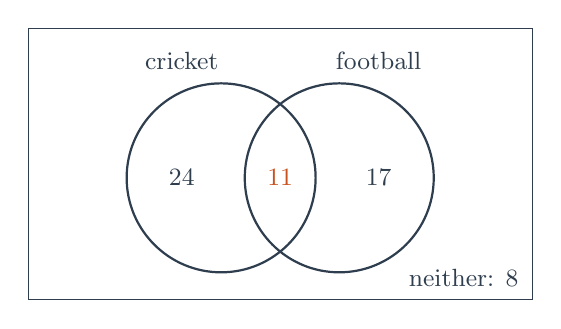
\begin{tikzpicture}[font=\small]
\draw[color=slate] (-3.2,-1.55) rectangle (3.2,1.9);
\draw[color=slate,thick] (-0.75,0) circle (1.2);
\draw[color=slate,thick] (0.75,0) circle (1.2);
\node[color=slate] at (-1.25,0) {24};
\node[color=ember] at (0,0) {11};
\node[color=slate] at (1.25,0) {17};
\node[color=slate,anchor=south east] at (3.15,-1.5) {neither: 8};
\node[color=slate,anchor=south] at (-1.25,1.25) {cricket};
\node[color=slate,anchor=south] at (1.25,1.25) {football};
\end{tikzpicture}\par\nopagebreak\smallskip
{\small Cricket only 24, both 11, football only 17, neither 8. Total $=24+11+17+8=60$.}
\end{center}

\samp 60 pupils, 35 play cricket, 28 play football, 8 play neither.
\begin{enumerate}
\item At least one: $60 - 8 = 52$.
\item Both $=35 + 28 - 52 = \mathbf{11}$.
\item Cricket only $=35 - 11 = 24$.
\item Football only $=28 - 11 = 17$.
\end{enumerate}
\samp Of 100 people, 50 like tea, 40 coffee and 30 milk. 20 like tea and coffee, 10 coffee and milk, 15 tea and milk, and 5 like all three. How many like none, and how many like tea only?
\begin{enumerate}
\item Union $=50 + 40 + 30 - 20 - 10 - 15 + 5 = 80$.
\item None $=100 - 80 = \mathbf{20}$.
\item Tea only $=50 - 20 - 15 + 5 = \mathbf{20}$ (take away both overlaps, then add back the all-three people you took away twice).
\end{enumerate}

\tryit Of 80 people, 45 speak Hindi, 38 speak English and 10 speak neither. (a) How many speak both? (b) How many speak only Hindi?

\subsection{Y12. Which diagram fits the classes?}
\spot ``Which diagram shows the relation among lions, tigers and animals?''

\mech Compare the three terms \textbf{two at a time}. For each pair ask: is one a kind of the other (circle inside)? Can something be both (circles overlap)? Can nothing be both (circles apart)? Then pick the picture.

\begin{center}
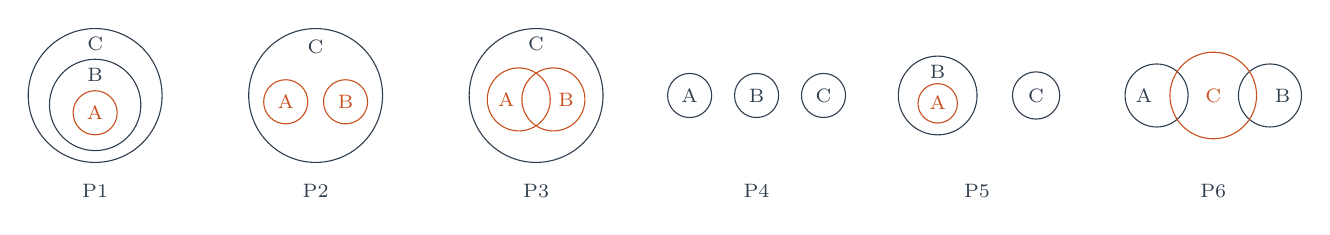
\begin{tikzpicture}[font=\scriptsize]
\begin{scope}
\draw[color=slate] (0,0) circle (0.85);
\draw[color=slate] (0,-0.12) circle (0.58);
\draw[color=ember] (0,-0.22) circle (0.28);
\node[color=slate] at (0,0.66) {C};
\node[color=slate] at (0,0.26) {B};
\node[color=ember] at (0,-0.22) {A};
\node[anchor=north,color=slate] at (0,-1.0) {P1};
\end{scope}
\begin{scope}[xshift=2.8cm]
\draw[color=slate] (0,0) circle (0.85);
\draw[color=ember] (-0.38,-0.08) circle (0.28);
\draw[color=ember] (0.38,-0.08) circle (0.28);
\node[color=slate] at (0,0.62) {C};
\node[color=ember] at (-0.38,-0.08) {A};
\node[color=ember] at (0.38,-0.08) {B};
\node[anchor=north,color=slate] at (0,-1.0) {P2};
\end{scope}
\begin{scope}[xshift=5.6cm]
\draw[color=slate] (0,0) circle (0.85);
\draw[color=ember] (-0.22,-0.05) circle (0.4);
\draw[color=ember] (0.22,-0.05) circle (0.4);
\node[color=slate] at (0,0.65) {C};
\node[color=ember] at (-0.38,-0.05) {A};
\node[color=ember] at (0.38,-0.05) {B};
\node[anchor=north,color=slate] at (0,-1.0) {P3};
\end{scope}
\begin{scope}[xshift=8.4cm]
\draw[color=slate] (-0.85,0) circle (0.28);
\draw[color=slate] (0,0) circle (0.28);
\draw[color=slate] (0.85,0) circle (0.28);
\node[color=slate] at (-0.85,0) {A};
\node[color=slate] at (0,0) {B};
\node[color=slate] at (0.85,0) {C};
\node[anchor=north,color=slate] at (0,-1.0) {P4};
\end{scope}
\begin{scope}[xshift=11.2cm]
\draw[color=slate] (-0.5,0) circle (0.5);
\draw[color=ember] (-0.5,-0.1) circle (0.25);
\draw[color=slate] (0.75,0) circle (0.3);
\node[color=slate] at (-0.5,0.3) {B};
\node[color=ember] at (-0.5,-0.1) {A};
\node[color=slate] at (0.75,0) {C};
\node[anchor=north,color=slate] at (0,-1.0) {P5};
\end{scope}
\begin{scope}[xshift=14.2cm]
\draw[color=slate] (-0.72,0) circle (0.4);
\draw[color=slate] (0.72,0) circle (0.4);
\draw[color=ember] (0,0) circle (0.55);
\node[color=slate] at (-0.88,0) {A};
\node[color=slate] at (0.88,0) {B};
\node[color=ember] at (0,0) {C};
\node[anchor=north,color=slate] at (0,-1.0) {P6};
\end{scope}
\end{tikzpicture}\par\nopagebreak\smallskip
{\small The six common patterns.}
\end{center}

\begin{center}\small\renewcommand{\arraystretch}{1.18}\setlength{\tabcolsep}{8pt}
\begin{tabularx}{\linewidth}{@{}l >{\raggedright\arraybackslash}X >{\raggedright\arraybackslash}X@{}}
\toprule
\textbf{\color{slate}Pattern} & \textbf{\color{slate}Meaning} & \textbf{\color{slate}Example} \\ \midrule
P1 & each inside the next & puppies, dogs, animals \\
P2 & two apart, both inside a third & lions, tigers, animals \\
P3 & two overlapping, both inside a third & doctors, teachers, persons \\
P4 & all three apart & cats, pens, rivers \\
P5 & one inside another, third apart & mangoes, fruits, vehicles \\
P6 & two apart, a third overlapping both & men, women, doctors \\
\bottomrule
\end{tabularx}\end{center}

\samp Lions, tigers, animals.
\begin{enumerate}
\item Lions and tigers: nothing is both, so apart.
\item Each is an animal, so inside. \textbf{P2}.
\end{enumerate}
\samp Doctors, teachers, persons.
\begin{enumerate}
\item A person can be both a doctor and a teacher, so overlap.
\item Both are persons. \textbf{P3}.
\end{enumerate}
\samp Mangoes, fruits, vehicles.
\begin{enumerate}
\item Mangoes are a kind of fruit (inside).
\item Vehicles share nothing with either (apart). \textbf{P5}.
\end{enumerate}

\tryit Which pattern fits (a) cats, dogs, animals? (b) teachers, men, women?

\subsection*{Shortcuts to memorise}
\begin{center}\small\renewcommand{\arraystretch}{1.9}\setlength{\tabcolsep}{8pt}
\begin{tabularx}{\linewidth}{@{}>{\raggedright\arraybackslash}X>{\raggedright\arraybackslash}X@{}}
\toprule
\textbf{\color{slate}Idea} & \textbf{\color{slate}Rule} \\ \midrule
Follows & true in every allowed picture \\
All A are B & also Some A are B and Some B are A, but not All B are A \\
Flips freely & Some A are B, No A is B \\
Never flips & Some A are not B \\
Pairs with a conclusion & the eight rows of the Y4 table \\
No conclusion & two ``some'' statements, two negatives, or a middle term that is never covered (Y5) \\
Either--or pairs & Some/No, All/Some not, Some/Some not \\
Only A are B & All B are A \\
Only some A are B & Some are, and some are not \\
Counting & $n(A\cup B)=n(A)+n(B)-n(A\cap B)$ \\
\bottomrule
\end{tabularx}\end{center}

\subsection*{Sanity checks before you mark the option}
\infobox{Ten seconds that save a wrong answer}{
\begin{itemize}
\item Did you try to \emph{break} the conclusion with a picture?
\item Does the conclusion use only terms that are in the statements?
\item Strong words (all, no, only, always) are the risky ones. Weak words (some, can be) are more often valid.
\item Did you ignore what you know about the real world?
\item If one conclusion already follows, either--or does not apply.
\end{itemize}}

\subsection*{Traps}
\begin{enumerate}
\item \textbf{Using real-world knowledge} instead of the statements.
\item \textbf{Turning ``All A are B'' into ``All B are A''} (Y2).
\item \textbf{Turning ``Some A are not B'' round} (Y2).
\item \textbf{Reading ``Only some'' as just ``some''} (Y9). It also says some are not.
\item \textbf{Drawing a conclusion from two ``some'' statements} (Y5).
\item \textbf{Chaining ``Some A are not B'' with ``All B are C'' into ``Some A are not C''} (Y5). That pair is not in the table.
\item \textbf{``No A is B'' and ``All B are C'' giving ``No A is C''} (Y4). Only ``Some C are not A'' follows.
\item \textbf{Drawing one picture only.} Test the loosest picture (Y6).
\item \textbf{Either--or when one conclusion already follows} (Y7).
\item \textbf{Either--or for All / No.} Both can be false (Y7).
\item \textbf{Counting the overlap twice} in a Venn count (Y11).
\item \textbf{Reading ``only A are B'' as ``All A are B''.} It flips (Y9).
\end{enumerate}

\subsection*{Answers to ``Try it''}
\begin{center}\small\renewcommand{\arraystretch}{1.2}\setlength{\tabcolsep}{8pt}
\begin{tabularx}{\linewidth}{@{}l>{\raggedright\arraybackslash}X>{\raggedright\arraybackslash}X@{}}
\toprule
\textbf{\color{slate}Type} & \textbf{\color{slate}Answer} & \textbf{\color{slate}Reason} \\ \midrule
Y1 & (a) yes \newline (b) no & (a) No A is B also gives Some B are not A \newline (b) ``Some are not'' does not turn round \\
Y2 & (a) yes \newline (b) no, then yes & (a) Some turns round \newline (b) All A are B gives only Some B are A \\
Y3 & only I & All dogs are living things follows; the reverse does not \\
Y4 & (a) yes \newline (b) yes \newline (c) yes & (a) Some + All gives Some A are C \newline (b) No + Some gives Some C are not A \newline (c) a tiger outside the animals is outside the lions too \\
Y5 & (a) no \newline (b) no & (a) ``dogs'' is only the big side of both ``All'' statements \newline (b) two negative statements \\
Y6 & (a) yes \newline (b) no & (a) the A that are C are in B \newline (b) the C in B may lie outside A \\
Y7 & either I or II & Some / No is a complementary pair, and neither follows alone \\
Y8 & (a) yes \newline (b) yes, then no & (a) Some + All, then Some + All \newline (b) Y and W are linked through Z, but X is not \\
Y9 & (a) yes \newline (b) no & ``Only teachers are readers'' means All readers are teachers \\
Y10 & (a) true \newline (b) false & (a) tables are chairs, so some chairs are tables \newline (b) the statement says every table is a chair \\
Y11 & (a) 13 \newline (b) 32 & (a) $45 + 38 - (80 - 10)$ \newline (b) $45 - 13$ \\
Y12 & (a) P2 \newline (b) P6 & (a) cats and dogs apart, both animals \newline (b) men and women apart, teachers overlap both \\
\bottomrule
\end{tabularx}\end{center}

\clearpage
\section[Directions (D1--D12)]{Directions (with turns, distances and shadows)}\label{ch:D}
\addtocontents{toc}{\protect\nopagebreak}

\subsection*{The one idea}
Direction questions are map questions. Put the start in the middle of a cross, north at the top and east on the right. Draw every leg as an arrow along the cross, then read the answer off the picture. North, east, south and west never change. \emph{Left} and \emph{right} depend on which way the person is facing, so turn every ``turns left'' and ``turns right'' into a compass direction before you move.

\begin{center}
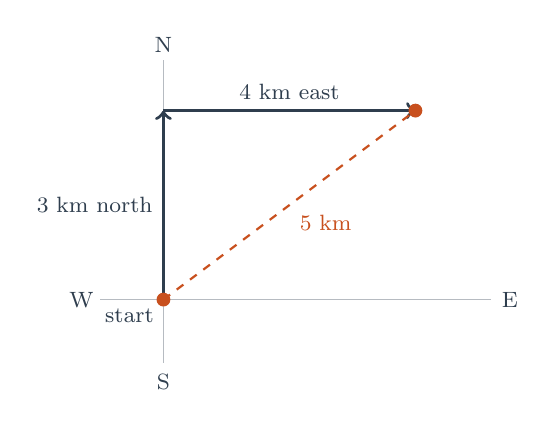
\begin{tikzpicture}[x=0.8cm,y=0.8cm,font=\footnotesize]
\draw[color=slate!35] (-1,0) -- (5.2,0);
\draw[color=slate!35] (0,-1) -- (0,3.8);
\node[color=slate] at (0,4.05) {N};
\node[color=slate] at (5.5,0) {E};
\node[color=slate] at (0,-1.3) {S};
\node[color=slate] at (-1.3,0) {W};
\draw[->,very thick,color=slate] (0,0) -- (0,3) node[midway,left] {3 km north};
\draw[->,very thick,color=slate] (0,3) -- (4,3) node[midway,above] {4 km east};
\draw[dashed,thick,color=ember] (0,0) -- (4,3) node[pos=0.5,below right] {5 km};
\fill[color=ember] (0,0) circle (2.5pt) node[anchor=north east,color=slate] {start};
\fill[color=ember] (4,3) circle (2.5pt);
\end{tikzpicture}\par\nopagebreak\smallskip
{\small Walk 3 km north, turn right, walk 4 km east. The finish is 5 km from the start, to its north-east.}
\end{center}

\infobox{Three habits that remove most mistakes}{
\begin{enumerate}
\item \textbf{Draw it.} Start in the middle of a cross with north at the top. A sketch catches most slips.
\item \textbf{Turn from the way he faces now}, not from where he started. Write every leg as a compass direction.
\item \textbf{Add east and west together, and north and south together.} Only then use Pythagoras.
\end{enumerate}}

\subsection*{Spot-it table}
Read the wording, find the row, jump to the type.
\begin{center}\small\renewcommand{\arraystretch}{1.18}\setlength{\tabcolsep}{7pt}
\begin{tabularx}{\linewidth}{@{}>{\raggedright\arraybackslash}X l >{\raggedright\arraybackslash}X@{}}
\toprule
\textbf{\color{slate}Wording in the question} & \textbf{\color{slate}Type} & \textbf{\color{slate}The one move} \\ \midrule
Facing south-west, which way is his right & D1 & read it off the wheel \\
Right, right, left, right: which way now & D2 & right $+1$, left $-1$, divide by 4 \\
Turns 135$^\circ$ clockwise, then 90$^\circ$ anticlockwise & D3 & add and subtract degrees \\
Walks 5 km north, turns right, walks 3 km & D4 & make every leg a compass leg \\
How far is he from the starting point & D5 & add each axis separately \\
24 m north, then 7 m east: how far from the start & D6 & Pythagoras, spot the triple \\
In which direction is he from the start & D7 & signs of the two totals \\
A walks north at 4 km/h, B east at 3 km/h & D8 & distance each, then compare \\
A is north of B, C is east of B: where is A from C & D9 & place them on a cross \\
At sunrise his shadow falls on his right & D10 & a shadow points away from the sun \\
A and B face each other: B's left hand & D11 & they face opposite ways \\
12 on a clock points north: the hour hand at 3 & D12 & 30$^\circ$ an hour, 6$^\circ$ a minute \\
\bottomrule
\end{tabularx}\end{center}

\subsection{D1. The compass wheel: directions, opposites, left and right}
\spot ``Facing south-west, which direction is on his right?'' ``What is opposite to north-east?'' ``Which direction lies between south and west?''

\mech
\begin{enumerate}
\item The eight directions go round a wheel, 45$^\circ$ apart, clockwise from north: north 0$^\circ$, north-east 45$^\circ$, east 90$^\circ$, south-east 135$^\circ$, south 180$^\circ$, south-west 225$^\circ$, west 270$^\circ$, north-west 315$^\circ$.
\item \textbf{Opposite} is half a turn (180$^\circ$) away: north--south, east--west, north-east--south-west, north-west--south-east.
\item Facing a direction: \textbf{right} is 90$^\circ$ clockwise (two steps round the wheel), \textbf{left} is 90$^\circ$ anticlockwise (two steps back), \textbf{behind} is 180$^\circ$.
\end{enumerate}

\begin{center}
\begin{minipage}[c]{0.40\linewidth}\centering
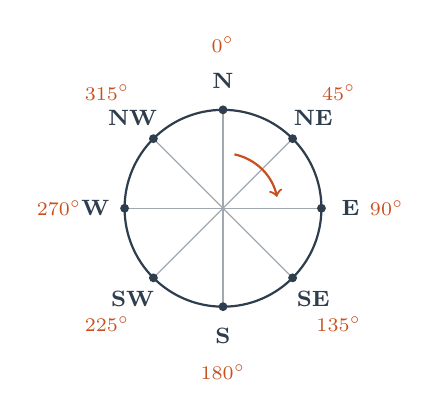
\begin{tikzpicture}[font=\footnotesize]
\draw[color=slate,thick] (0,0) circle (1.25);
\foreach \an/\nn/\bb in {90/N/0,45/NE/45,0/E/90,-45/SE/135,-90/S/180,-135/SW/225,180/W/270,135/NW/315}{
  \draw[color=slate!45] (0,0) -- (\an:1.25);
  \fill[color=slate] (\an:1.25) circle (1.6pt);
  \node[color=slate] at (\an:1.62) {\textbf{\nn}};
  \node[color=ember,font=\scriptsize] at (\an:2.08) {\bb$^\circ$};
}
\draw[->,color=ember,thick] (78:0.7) arc (78:12:0.7);
\end{tikzpicture}
\end{minipage}\hfill
\begin{minipage}[c]{0.56\linewidth}\centering
\small\renewcommand{\arraystretch}{1.18}\setlength{\tabcolsep}{6pt}
\begin{tabular}{@{}llll@{}}
\toprule
\textbf{\color{slate}Facing} & \textbf{\color{slate}Right} & \textbf{\color{slate}Left} & \textbf{\color{slate}Behind} \\ \midrule
north & east & west & south \\
north-east & south-east & north-west & south-west \\
east & south & north & west \\
south-east & south-west & north-east & north-west \\
south & west & east & north \\
south-west & north-west & south-east & north-east \\
west & north & south & east \\
north-west & north-east & south-west & south-east \\
\bottomrule
\end{tabular}
\end{minipage}
\par\medskip
{\small The wheel (angles run clockwise from north, 45$^\circ$ a step) and where each facing direction's right, left and back lie.}
\end{center}

\samp Facing south-west, which direction is on his right?
\begin{enumerate}
\item South-west is 225$^\circ$.
\item Right is $+90^\circ$: $225 + 90 = 315$, which is \textbf{north-west}.
\item (Left is 135$^\circ$, south-east. Behind is 45$^\circ$, north-east.)
\end{enumerate}
\samp What is opposite to north-east?
\begin{enumerate}
\item $45 + 180 = 225$, which is \textbf{south-west}.
\end{enumerate}
\samp Which direction lies half-way between south and west?
\begin{enumerate}
\item Half-way between 180$^\circ$ and 270$^\circ$ is 225$^\circ$: \textbf{south-west}.
\end{enumerate}

\tryit (a) Facing north-west, which direction is on his left? (b) What is opposite to south-east? (c) Which direction lies between east and south?

\subsection{D2. Facing after turns (right, left, about-turn)}
\spot ``Facing north, he turns right, then right, then left, then right. Which way is he facing now?''

\mech
\begin{enumerate}
\item Count each \textbf{right} turn as $+1$ and each \textbf{left} turn as $-1$ (a quarter turn each). An about-turn (a U-turn, ``turns back'') is $+2$.
\item Add them up and throw away whole circles of 4. The remainder (0, 1, 2 or 3; add 4 first if the total is negative) says where he ends up compared with the start:
\end{enumerate}
\begin{center}\small\renewcommand{\arraystretch}{1.18}\setlength{\tabcolsep}{9pt}
\begin{tabular}{@{}lllll@{}}
\toprule
\textbf{\color{slate}Remainder} & 0 & 1 & 2 & 3 \\ \midrule
\textbf{\color{slate}He faces} & the start direction & to its right & opposite to it & to its left \\
\bottomrule
\end{tabular}\end{center}
A right turn and a left turn cancel, and four turns the same way bring him back.

\samp Facing north: right, right, left, right.
\begin{enumerate}
\item $+1 + 1 - 1 + 1 = +2$.
\item Remainder 2 means opposite to the start: \textbf{south}.
\end{enumerate}
\samp Facing east: left, left, left, right, about-turn.
\begin{enumerate}
\item $-1 - 1 - 1 + 1 + 2 = 0$.
\item Back to the start direction: \textbf{east}.
\item (Step by step: east, north, west, south, west, east.)
\end{enumerate}
\samp Facing west: seven right turns.
\begin{enumerate}
\item $7 \div 4$ leaves 3.
\item Remainder 3 means to the left of the start.
\item Left of west is \textbf{south}.
\end{enumerate}

\tryit (a) Facing south: left, left, left, right. (b) Facing east: five right turns and three left turns.

\subsection{D3. Turning by an angle}
\spot ``Facing north-east, he turns 135$^\circ$ clockwise, then 90$^\circ$ anticlockwise.'' ``What is the smallest turn from north-east to south?''

\mech
\begin{enumerate}
\item \textbf{Clockwise} adds degrees (it is a right turn). \textbf{Anticlockwise} subtracts (a left turn). Start from the wheel angle of the way he faces (D1).
\item Add or subtract 360$^\circ$ until the answer is between 0$^\circ$ and 360$^\circ$, then read the direction off the wheel.
\item The turn from one direction to another is the difference of their angles. If it is more than 180$^\circ$, the other way round is shorter: the smallest turn is $360^\circ$ minus the difference, in the opposite sense.
\end{enumerate}

\samp Facing north-east, he turns 135$^\circ$ clockwise, then 90$^\circ$ anticlockwise.
\begin{enumerate}
\item $45 + 135 = 180$ (south).
\item Then $180 - 90 = 90$: \textbf{east}.
\end{enumerate}
\samp Facing west, he turns 225$^\circ$ anticlockwise.
\begin{enumerate}
\item $270 - 225 = 45$: \textbf{north-east}.
\end{enumerate}
\samp The smallest turn from north-east to south, and from south-west to north.
\begin{enumerate}
\item North-east to south: $180 - 45 = 135^\circ$ clockwise (anticlockwise would be $225^\circ$). \textbf{135$^\circ$ clockwise.}
\item South-west to north: clockwise it is $360 - 225 = 135^\circ$, anticlockwise it is $225^\circ$. \textbf{135$^\circ$ clockwise.}
\end{enumerate}

\tryit (a) Facing south-east, he turns 270$^\circ$ clockwise. Which way does he face? (b) What is the smallest turn, and in which sense, from north-east to west?

\subsection{D4. Walks with turns}
\spot ``Meera walks 5 km north, turns right and walks 3 km, turns right and walks 5 km.''

\mech
\begin{enumerate}
\item Find the way he faces on the first leg (the leg itself usually says it).
\item Before each leg, turn from the way he faces \emph{now}, not from where he started: right is a quarter turn clockwise, left a quarter turn anticlockwise (D2).
\item Write each leg as a compass direction and a distance. It is now a D5 problem.
\end{enumerate}

\begin{center}
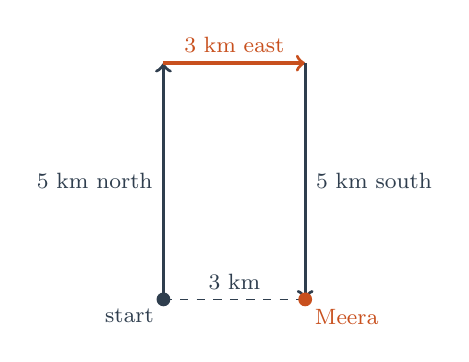
\begin{tikzpicture}[x=0.6cm,y=0.6cm,font=\footnotesize]
\draw[->,very thick,color=slate] (0,0) -- (0,5) node[midway,left] {5 km north};
\draw[->,very thick,color=ember] (0,5) -- (3,5) node[midway,above] {3 km east};
\draw[->,very thick,color=slate] (3,5) -- (3,0) node[midway,right] {5 km south};
\draw[dashed,color=slate] (0,0) -- (3,0) node[midway,above] {3 km};
\fill[color=slate] (0,0) circle (2.5pt) node[anchor=north east] {start};
\fill[color=ember] (3,0) circle (2.5pt) node[anchor=north west] {Meera};
\end{tikzpicture}\par\nopagebreak\smallskip
{\small Two right turns send her east, then south. The north and south legs cancel, so she ends 3 km east of the start.}
\end{center}

\samp Meera walks 5 km north, turns right and walks 3 km, turns right and walks 5 km. Which way does she face at the end, and where is she from the start?
\begin{enumerate}
\item North 5 km.
\item Right from north is east: east 3 km.
\item Right from east is south: south 5 km.
\item She faces \textbf{south}.
\item The north and south legs cancel, so she is \textbf{3 km east} of the start.
\end{enumerate}
\samp A man walks 12 m south, turns left and walks 8 m, turns right and walks 4 m, turns right and walks 8 m. Which way does he face at the end, and where is he from the start?
\begin{enumerate}
\item South 12.
\item Left from south is east: east 8.
\item Right from east is south: south 4.
\item Right from south is west: west 8.
\item East 8 and west 8 cancel, so he is $12 + 4 =$ \textbf{16 m south} of the start, facing \textbf{west}.
\end{enumerate}

\tryit Facing north, Asha walks 7 km, turns left and walks 4 km, turns left and walks 7 km. Which way is she facing at the end, and where is she from the start?

\subsection{D5. Net position: add each axis separately}
\spot ``How far is he from the starting point?'' after several legs in different directions.

\mech
\begin{enumerate}
\item Start at $(0,0)$. East is $+$ and west is $-$ (that is $x$). North is $+$ and south is $-$ (that is $y$).
\item Add all the east--west legs for $x$ and all the north--south legs for $y$. Never mix the two.
\item If $x$ or $y$ is 0, he is on a straight line from the start: the distance is the other number, without its sign. If neither is 0, the distance is $\sqrt{x^2+y^2}$ (D6).
\item Distance \emph{walked} is different: add every leg, ignoring directions. It is never less than the distance from the start.
\end{enumerate}

\begin{center}
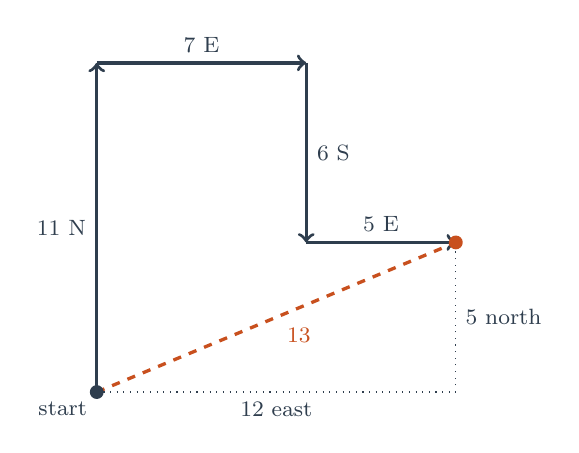
\begin{tikzpicture}[x=0.38cm,y=0.38cm,font=\footnotesize]
\draw[->,very thick,color=slate] (0,0) -- (0,11) node[midway,left] {11 N};
\draw[->,very thick,color=slate] (0,11) -- (7,11) node[midway,above] {7 E};
\draw[->,very thick,color=slate] (7,11) -- (7,5) node[midway,right] {6 S};
\draw[->,very thick,color=slate] (7,5) -- (12,5) node[midway,above] {5 E};
\draw[dashed,very thick,color=ember] (0,0) -- (12,5) node[pos=0.5,below right] {13};
\draw[dotted,color=slate] (0,0) -- (12,0) node[midway,below] {12 east};
\draw[dotted,color=slate] (12,0) -- (12,5) node[midway,right] {5 north};
\fill[color=slate] (0,0) circle (2.5pt) node[anchor=north east] {start};
\fill[color=ember] (12,5) circle (2.5pt);
\end{tikzpicture}\par\nopagebreak\smallskip
{\small The four legs and the straight line back to the start. They add up to 12 east and 5 north, so the line is 13.}
\end{center}

\samp He walks 11 m north, 7 m east, 6 m south, then 5 m east. How far is he from the start, and how far did he walk?
\begin{enumerate}
\item $x = 7 + 5 = 12$ east. $y = 11 - 6 = 5$ north.
\item From the start: $\sqrt{12^2 + 5^2} = \mathbf{13}$ m (the 5, 12, 13 triple).
\item Walked: $11 + 7 + 6 + 5 = \mathbf{29}$ m.
\end{enumerate}
\samp West 9 m, south 4 m, east 9 m, north 4 m.
\begin{enumerate}
\item $x = -9 + 9 = 0$ and $y = -4 + 4 = 0$.
\item He is \textbf{back at the start} (distance 0) after walking 26 m.
\end{enumerate}
\samp East 20 m, north 3 m, west 5 m, north 5 m.
\begin{enumerate}
\item $x = 20 - 5 = 15$. $y = 3 + 5 = 8$.
\item From the start: $\sqrt{15^2 + 8^2} = \mathbf{17}$ m (the 8, 15, 17 triple).
\item He walked 33 m.
\end{enumerate}

\tryit (a) West 16 m, south 2 m, east 4 m, south 3 m: how far from the start, and how far walked? (b) East 7 m, north 24 m, west 14 m, south 24 m: how far from the start, and how far walked?

\subsection{D6. Right-angle distances (Pythagoras and triples)}
\spot ``24 m north, then 7 m east: how far is he from the start?'' ``How much shorter is the direct path?'' ``5 km north, then some km east, and he ends 13 km from the start: how far east?''

\mech
\begin{enumerate}
\item Two legs at right angles are the short sides of a right triangle. The distance from the start is the long side: $d^2 = a^2 + b^2$.
\item Learn the whole-number triples in the table below and their multiples. Spot them before you square anything.
\end{enumerate}
\begin{center}\small\renewcommand{\arraystretch}{1.18}\setlength{\tabcolsep}{9pt}
\begin{tabular}{@{}lllll@{}}
\toprule
\textbf{\color{slate}Triple} & \textbf{\color{slate}$\times 2$} & \textbf{\color{slate}$\times 3$} & \textbf{\color{slate}$\times 4$} & \textbf{\color{slate}$\times 5$} \\ \midrule
3, 4, 5 & 6, 8, 10 & 9, 12, 15 & 12, 16, 20 & 15, 20, 25 \\
5, 12, 13 & 10, 24, 26 & 15, 36, 39 & & \\
8, 15, 17 & 16, 30, 34 & & & \\
7, 24, 25 & 14, 48, 50 & & & \\
20, 21, 29 & & & & \\
\bottomrule
\end{tabular}\end{center}
\begin{enumerate}
\setcounter{enumi}{2}
\item \textbf{Route saved} by cutting across $= (a + b) - d$.
\item \textbf{Missing leg:} $b^2 = d^2 - a^2$. Look for the triple again.
\end{enumerate}

\samp 24 m north, then 7 m east. How far is he from the start?
\begin{enumerate}
\item The 7, 24, 25 triple: \textbf{25 m}.
\item (Check: $576 + 49 = 625$.)
\end{enumerate}
\samp 15 km east, then 8 km north. How much shorter is the direct path than the two legs?
\begin{enumerate}
\item The 8, 15, 17 triple: the direct path is 17 km.
\item The legs add up to $15 + 8 = 23$ km.
\item Saved: $23 - 17 = \mathbf{6}$ km.
\end{enumerate}
\samp He walks 5 km north, then some km east, and ends 13 km from the start. How far east did he walk?
\begin{enumerate}
\item 13 is the long side and 5 a short side: the 5, 12, 13 triple, so \textbf{12 km}.
\item (Check: $169 - 25 = 144$.)
\end{enumerate}

\tryit (a) 16 m west, then 12 m south: how far from the start? (b) 9 km north, then some km west, and he ends 15 km from the start: how far west did he walk?

\subsection{D7. Which direction is he from the start?}
\spot ``In which direction is he from the starting point?'' ``Which way must he walk to get back to the start?''

\mech
\begin{enumerate}
\item Get $x$ and $y$ as in D5.
\item Read the signs:
\end{enumerate}
\begin{center}\small\renewcommand{\arraystretch}{1.18}\setlength{\tabcolsep}{9pt}
\begin{tabular}{@{}lll@{}}
\toprule
\textbf{\color{slate}$x$ (east $+$)} & \textbf{\color{slate}$y$ (north $+$)} & \textbf{\color{slate}He is to the} \\ \midrule
$+$ & $+$ & north-east \\
$+$ & $-$ & south-east \\
$-$ & $-$ & south-west \\
$-$ & $+$ & north-west \\
0 & $+$ or $-$ & north or south \\
$+$ or $-$ & 0 & east or west \\
\bottomrule
\end{tabular}\end{center}
\begin{enumerate}
\setcounter{enumi}{2}
\item \textbf{The way back} is the opposite direction (D1), over the same distance.
\item Exams use only the eight directions, so 3 m east and 10 m north is still ``north-east''.
\end{enumerate}

\samp The finish is 12 m east and 5 m north of the start.
\begin{enumerate}
\item East and north: \textbf{north-east}.
\item To get back he walks \textbf{south-west}.
\end{enumerate}
\samp The finish is 16 m south of the start, in line with it (no east or west).
\begin{enumerate}
\item $x = 0$ and $y$ is south: \textbf{south}.
\item The way back is \textbf{north}.
\end{enumerate}
\samp He walks 8 m west, then 6 m south. Where is the start from him?
\begin{enumerate}
\item $x = -8$, $y = -6$: he is \textbf{south-west} of the start, so the start is \textbf{north-east} of him.
\end{enumerate}

\tryit He walks 14 m east, 10 m north, 6 m west and 15 m south. (a) In which direction is he from the start? (b) Which way must he walk to get back?

\subsection{D8. Two people from the same point}
\spot ``A walks north at 4 km/h and B walks east at 3 km/h. How far apart are they after 2 hours?''

\mech
\begin{enumerate}
\item Each distance is speed $\times$ time (chapter 2).
\item \textbf{Same direction:} subtract the distances. \textbf{Opposite directions:} add them. \textbf{At right angles:} Pythagoras (D6).
\item If one of them starts later, use that person's own walking time.
\end{enumerate}

\samp A walks north at 4 km/h and B walks east at 3 km/h. How far apart are they after 2 hours?
\begin{enumerate}
\item A: $4 \times 2 = 8$ km north.
\item B: $3 \times 2 = 6$ km east.
\item At right angles: the 6, 8, 10 triple, so \textbf{10 km} apart.
\end{enumerate}
\samp A walks east at 5 km/h and B walks west at 7 km/h. How far apart after 3 hours?
\begin{enumerate}
\item $15 + 21 = \mathbf{36}$ km (opposite directions: add).
\end{enumerate}
\samp Both walk north: A at 6 km/h and B at 4 km/h. How far apart after 5 hours?
\begin{enumerate}
\item $30 - 20 = \mathbf{10}$ km (same direction: subtract).
\item A is ahead.
\end{enumerate}

\tryit (a) A cyclist goes south at 12 km/h and another goes west at 16 km/h, from the same point. How far apart are they after 3 hours? (b) A goes north at 9 km/h and B goes south at 6 km/h from the same point. After how many hours are they 60 km apart?

\subsection{D9. Relative positions of places or people}
\spot ``A is north of B, and C is east of B. In which direction is A from C?''

\mech
\begin{enumerate}
\item Draw a cross and put the first named point in the middle.
\item Add each next point with an arrow from one already placed. ``A is north of B'' also means B is south of A.
\item To find the direction of P \emph{from} Q, go from Q to P and read the east--west and north--south steps, as in D7. If distances are given, D6 gives the distance between them.
\end{enumerate}

\begin{center}
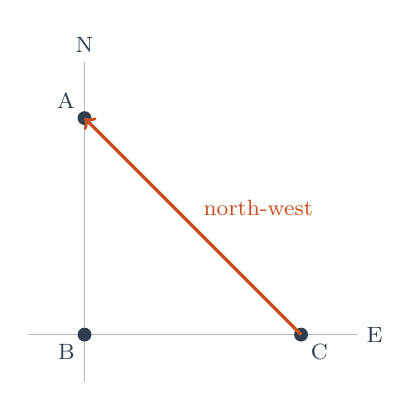
\begin{tikzpicture}[x=0.55cm,y=0.55cm,font=\footnotesize]
\draw[color=slate!35] (-1.3,0) -- (6.3,0);
\draw[color=slate!35] (0,-1.1) -- (0,6.3);
\node[color=slate] at (0,6.7) {N};
\node[color=slate] at (6.7,0) {E};
\fill[color=slate] (0,0) circle (2.5pt) node[anchor=north east] {B};
\fill[color=slate] (0,5) circle (2.5pt) node[anchor=south east] {A};
\fill[color=slate] (5,0) circle (2.5pt) node[anchor=north west] {C};
\draw[->,very thick,color=ember] (5,0) -- (0,5) node[midway,above right] {north-west};
\end{tikzpicture}\par\nopagebreak\smallskip
{\small B in the middle, A 5 m above it, C 5 m to its right. The arrow from C to A points north-west.}
\end{center}

\samp A is 5 m north of B. C is 5 m east of B. In which direction is A from C?
\begin{enumerate}
\item B in the middle, A 5 m above it, C 5 m to its right.
\item From C to A: 5 m west and 5 m north: \textbf{north-west}.
\end{enumerate}
\samp P is 8 m west of Q. R is 6 m south of Q. How far is P from R, and in which direction is P from R?
\begin{enumerate}
\item Q in the middle, P 8 m to its left, R 6 m below.
\item From R to P: 8 m west and 6 m north.
\item Distance: the 6, 8, 10 triple, \textbf{10 m}, to the \textbf{north-west}.
\end{enumerate}
\samp X is south of Y. Z is west of Y. In which direction is Z from X?
\begin{enumerate}
\item Y in the middle, X below it, Z to its left.
\item From X to Z: west and north: \textbf{north-west}.
\item (No distances are needed; the signs decide.)
\end{enumerate}

\tryit (a) M is 12 m east of N. L is 5 m north of N. How far is L from M, and in which direction is L from M? (b) S is west of T, and T is south of U. In which direction is U from S?

\subsection{D10. Shadows}
\spot ``At sunrise, Ravi's shadow falls on his right. Which way is he facing?''

\mech
\begin{enumerate}
\item The sun rises in the east and sets in the west. A shadow points \emph{away} from the sun: in the \textbf{morning it falls to the west}, in the \textbf{evening to the east}. (Ignore noon: the shadow is under him.)
\item Then use where the shadow falls, compared with him, to find the way he faces:
\end{enumerate}
\begin{center}\small\renewcommand{\arraystretch}{1.18}\setlength{\tabcolsep}{9pt}
\begin{tabular}{@{}ll@{}}
\toprule
\textbf{\color{slate}The shadow falls} & \textbf{\color{slate}He faces} \\ \midrule
in front of him & the way the shadow points \\
behind him & the opposite way \\
on his right & a quarter turn anticlockwise from the shadow's direction \\
on his left & a quarter turn clockwise from the shadow's direction \\
\bottomrule
\end{tabular}\end{center}
\begin{enumerate}
\setcounter{enumi}{2}
\item Two people standing back to back face opposite ways.
\end{enumerate}

\begin{center}
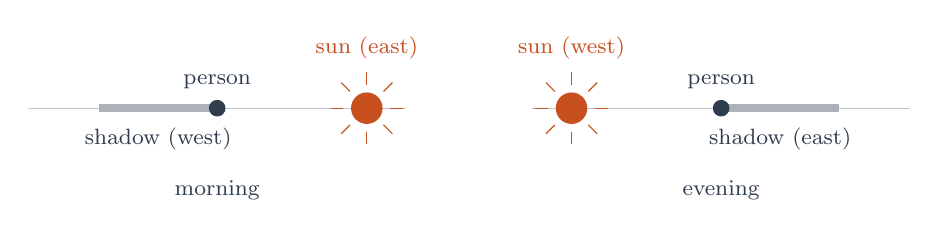
\begin{tikzpicture}[font=\footnotesize]
\begin{scope}
\draw[color=slate!30] (-2.4,0) -- (2.4,0);
\fill[color=ember] (1.9,0) circle (0.2);
\foreach \r in {0,45,...,315}{\draw[color=ember] (1.9,0) ++(\r:0.3) -- ++(\r:0.16);}
\node[color=ember,anchor=south] at (1.9,0.5) {sun (east)};
\draw[line width=3pt,color=slate!40] (0,0) -- (-1.5,0);
\node[color=slate,anchor=north] at (-0.75,-0.12) {shadow (west)};
\fill[color=slate] (0,0) circle (3pt);
\node[color=slate,anchor=south] at (0,0.12) {person};
\node[color=slate,anchor=north] at (0,-0.8) {morning};
\end{scope}
\begin{scope}[xshift=6.4cm]
\draw[color=slate!30] (-2.4,0) -- (2.4,0);
\fill[color=ember] (-1.9,0) circle (0.2);
\foreach \r in {0,45,...,315}{\draw[color=ember] (-1.9,0) ++(\r:0.3) -- ++(\r:0.16);}
\node[color=ember,anchor=south] at (-1.9,0.5) {sun (west)};
\draw[line width=3pt,color=slate!40] (0,0) -- (1.5,0);
\node[color=slate,anchor=north] at (0.75,-0.12) {shadow (east)};
\fill[color=slate] (0,0) circle (3pt);
\node[color=slate,anchor=south] at (0,0.12) {person};
\node[color=slate,anchor=north] at (0,-0.8) {evening};
\end{scope}
\end{tikzpicture}\par\nopagebreak\smallskip
{\small Seen from above, north at the top. The shadow always points away from the sun.}
\end{center}

\samp At sunrise Ravi stands facing the sun. Where does his shadow fall?
\begin{enumerate}
\item The sun is in the east, so he faces east.
\item The shadow points west, \textbf{behind him}.
\end{enumerate}
\samp In the morning Asha's shadow falls on her right. Which way is she facing?
\begin{enumerate}
\item Morning shadow: west.
\item On her right: a quarter turn anticlockwise from west is south.
\item She faces \textbf{south}.
\item (Check: facing south, her right hand is west.)
\end{enumerate}
\samp At sunset two friends stand back to back. Mohan's shadow falls on his left. Which way does each face?
\begin{enumerate}
\item Evening shadow: east.
\item On his left: a quarter turn clockwise from east is south.
\item Mohan faces \textbf{south} and the other friend faces \textbf{north}.
\end{enumerate}

\tryit (a) At sunset, Ria's shadow falls behind her. Which way does she face? (b) In the morning, Sam's shadow falls on his left. Which way does he face?

\subsection{D11. Facing each other}
\spot ``A and B stand facing each other. A faces east. In which direction does B's right hand point?''

\mech
\begin{enumerate}
\item People who face each other, or stand back to back, face opposite directions (D1).
\item Work out each person's left and right from their own facing direction (D1).
\item So A's right hand and B's left hand point the same compass way, and A's right and B's right point opposite ways. Two people facing the same way share left and right.
\end{enumerate}

\samp A faces east and B stands facing A. In which direction does B's right hand point?
\begin{enumerate}
\item B faces west.
\item Right of west is \textbf{north}.
\item (A's left hand also points north.)
\end{enumerate}
\samp Two people stand back to back. One faces south-east. Which way does the other face, and which way is the other's right hand?
\begin{enumerate}
\item The other faces north-west.
\item Right of north-west is \textbf{north-east}.
\end{enumerate}
\samp P faces north and Q stands behind P, also facing north. In which direction is Q's left hand?
\begin{enumerate}
\item Same facing, same sides: Q's left hand points \textbf{west}.
\end{enumerate}

\tryit (a) A faces west and B stands facing A. In which direction does B's left hand point? (b) Two people stand back to back, one facing south-west. In which direction does the other's right hand point?

\subsection{D12. Directions on a clock face}
\spot ``The 12 on a clock points north. In which direction does the hour hand point at 3 o'clock?''

\mech
\begin{enumerate}
\item A clock face is a wheel read clockwise from the 12. 12 hours is 360$^\circ$, so \textbf{30$^\circ$ an hour}. 60 minutes is 360$^\circ$, so \textbf{6$^\circ$ a minute}.
\item A hand's direction is the direction of the 12 plus the hand's angle from the 12 (add, as for a clockwise turn in D3).
\item The hour hand at $h$ o'clock is $30h$ degrees from the 12 (half past adds 15$^\circ$). The minute hand at $m$ minutes is $6m$.
\end{enumerate}

\begin{center}
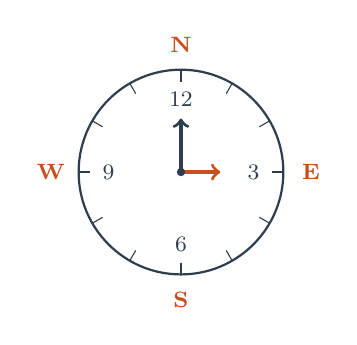
\begin{tikzpicture}[font=\footnotesize]
\draw[color=slate,thick] (0,0) circle (1.3);
\foreach \h in {0,...,11}{
  \draw[color=slate] (90-\h*30:1.15) -- (90-\h*30:1.3);
}
\node[color=slate] at (90:0.92) {12};
\node[color=slate] at (0:0.92) {3};
\node[color=slate] at (-90:0.92) {6};
\node[color=slate] at (180:0.92) {9};
\node[color=ember] at (90:1.62) {\textbf{N}};
\node[color=ember] at (0:1.65) {\textbf{E}};
\node[color=ember] at (-90:1.62) {\textbf{S}};
\node[color=ember] at (180:1.65) {\textbf{W}};
\draw[->,very thick,color=slate] (0,0) -- (90:0.68);
\draw[->,very thick,color=ember] (0,0) -- (0:0.5);
\fill[color=slate] (0,0) circle (1.5pt);
\end{tikzpicture}\par\nopagebreak\smallskip
{\small 12 at the top is north: 3 is east, 6 south, 9 west. At 3 o'clock the hour hand (ember) points east.}
\end{center}

\samp The 12 points north. Which way does the hour hand point at 3 o'clock?
\begin{enumerate}
\item $3 \times 30 = 90^\circ$ from the 12: \textbf{east}.
\end{enumerate}
\samp The 12 points north-east. Which way does the minute hand point at 45 minutes?
\begin{enumerate}
\item $45 \times 6 = 270^\circ$ from the 12.
\item North-east is 45$^\circ$: $45 + 270 = 315$, which is \textbf{north-west}.
\end{enumerate}
\samp The 12 points east. Which way does the hour hand point at 9 o'clock?
\begin{enumerate}
\item $9 \times 30 = 270^\circ$ from the 12.
\item East is 90$^\circ$: $90 + 270 = 360$, which is \textbf{north}.
\end{enumerate}

\tryit (a) The 12 points west. Which way does the hour hand point at 6 o'clock? (b) The 12 points north-west. Which way does the minute hand point at 15 minutes?

\subsection*{Shortcuts to memorise}
\begin{center}\small\renewcommand{\arraystretch}{1.9}\setlength{\tabcolsep}{8pt}
\begin{tabularx}{\linewidth}{@{}>{\raggedright\arraybackslash}X>{\raggedright\arraybackslash}X@{}}
\toprule
\textbf{\color{slate}Idea} & \textbf{\color{slate}Rule} \\ \midrule
The wheel & N 0$^\circ$, NE 45$^\circ$, E 90$^\circ$, SE 135$^\circ$, S 180$^\circ$, SW 225$^\circ$, W 270$^\circ$, NW 315$^\circ$ \\
Right, left, about-turn & $+90^\circ$, $-90^\circ$, $180^\circ$ \\
Quarter turns & right $+1$, left $-1$, about-turn $+2$; divide by 4 and keep the remainder \\
Clockwise or anticlockwise & clockwise is right (add), anticlockwise is left (subtract) \\
Net position & east and north $+$, west and south $-$; add each axis separately \\
Distance from the start & $\sqrt{x^2+y^2}$; learn 3-4-5, 5-12-13, 8-15-17, 7-24-25, 20-21-29 \\
Distance walked & add every leg; never less than the distance from the start \\
Direction from the start & signs of $x$ and $y$; the way back is the opposite \\
Two walkers & same way: subtract; opposite ways: add; right angles: Pythagoras \\
Shadows & morning: west; evening: east (away from the sun) \\
Facing each other & opposite directions; A's right is B's left \\
Clock face & 30$^\circ$ an hour, 6$^\circ$ a minute, clockwise from the 12 \\
\bottomrule
\end{tabularx}\end{center}

\subsection*{Sanity checks before you mark the option}
\infobox{Ten seconds that save a wrong answer}{
\begin{itemize}
\item Does your sketch end where your numbers say, with north at the top?
\item Is the distance from the start no more than the distance walked? If it is more, something is wrong.
\item Did every turn start from the way he was facing at that moment?
\item In a right triangle the distance from the start is the longest side. A leg can never be longer than it.
\item Does the shadow point away from the sun?
\end{itemize}}

\subsection*{Traps}
\begin{enumerate}
\item \textbf{Treating left and right as fixed directions.} They depend on the way he faces (D1, D2).
\item \textbf{Turning from the starting direction} instead of the direction he faces now (D4).
\item \textbf{Reading ``turns 270$^\circ$ clockwise'' as a right turn} (D3). It is three right turns, the same as one left turn.
\item \textbf{Mixing the axes}: adding a north leg to an east leg (D5).
\item \textbf{Giving the distance walked} when the question asks how far he is from the start (D5).
\item \textbf{Adding when the long side is known}: for a missing leg you subtract the squares (D6).
\item \textbf{Calling the finish ``north'' when it is also east} of the start (D7). Neither total being 0 means a diagonal.
\item \textbf{Giving the direction of him from the start when the question asks for the start from him} (D7). They are opposite.
\item \textbf{Using the wrong rule for two walkers} (D8): same way subtracts, opposite ways add, right angles need Pythagoras.
\item \textbf{Putting the shadow on the sun's side} (D10). It points away from the sun.
\item \textbf{Giving two people who face each other the same left and right} (D11).
\item \textbf{Mixing up the hour and minute angles} on the clock (D12): 30$^\circ$ an hour, 6$^\circ$ a minute.
\end{enumerate}

\subsection*{Answers to ``Try it''}
\begin{center}\small\renewcommand{\arraystretch}{1.2}\setlength{\tabcolsep}{8pt}
\begin{tabularx}{\linewidth}{@{}l>{\raggedright\arraybackslash}X>{\raggedright\arraybackslash}X@{}}
\toprule
\textbf{\color{slate}Type} & \textbf{\color{slate}Answer} & \textbf{\color{slate}Working} \\ \midrule
D1 & (a) south-west \newline (b) north-west \newline (c) south-east & (a) $315 - 90 = 225$ \newline (b) $135 + 180 = 315$ \newline (c) half-way between 90$^\circ$ and 180$^\circ$ is 135$^\circ$ \\
D2 & (a) north \newline (b) west & (a) $-3 + 1 = -2$, remainder 2: opposite of south \newline (b) $5 - 3 = 2$: opposite of east \\
D3 & (a) north-east \newline (b) 135$^\circ$ anticlockwise & (a) $135 + 270 = 405$, minus 360 is 45 \newline (b) clockwise is $270 - 45 = 225$, so the other way is $360 - 225 = 135$ \\
D4 & facing south; 4 km west of the start & north 7, west 4, south 7: the north and south legs cancel \\
D5 & (a) 13 m from the start, 25 m walked \newline (b) 7 m from the start, 69 m walked & (a) $x = -16 + 4 = -12$, $y = -2 - 3 = -5$, the 5, 12, 13 triple \newline (b) $x = 7 - 14 = -7$, $y = 24 - 24 = 0$ \\
D6 & (a) 20 m \newline (b) 12 km & (a) 3, 4, 5 times 4 \newline (b) 9, 12, 15 \\
D7 & (a) south-east \newline (b) north-west & $x = 14 - 6 = 8$, $y = 10 - 15 = -5$; the way back is the opposite \\
D8 & (a) 60 km \newline (b) 4 hours & (a) 36 and 48 at right angles, 3, 4, 5 times 12 \newline (b) they part by $9 + 6 = 15$ km an hour, and $60 \div 15 = 4$ \\
D9 & (a) 13 m, north-west \newline (b) north-east & (a) 12 west and 5 north from M to L, the 5, 12, 13 triple \newline (b) U is east of S and also north of S \\
D10 & (a) west \newline (b) north & (a) the evening shadow points east, so she faces the other way \newline (b) the morning shadow points west, on his left: a quarter turn clockwise \\
D11 & (a) north \newline (b) south-east & (a) B faces east, and left of east is north \newline (b) the other faces north-east, and right of north-east is south-east \\
D12 & (a) east \newline (b) north-east & (a) $270 + 180 = 450$, minus 360 is 90 \newline (b) $315 + 90 = 405$, minus 360 is 45 \\
\bottomrule
\end{tabularx}\end{center}

\clearpage
\section[Blood relations (B1--B12)]{Blood relations (with family trees and coded relations)}\label{ch:B}
\addtocontents{toc}{\protect\nopagebreak}

\subsection*{The one idea}
Blood relation questions are family trees told in words. Draw the tree: one row for each generation, parents above and children below, a double line between husband and wife. Mark every person as a man or a woman as soon as a word gives it away. Then read the answer off the tree: count the generations, check the side (father's or mother's), and name the person using their own sex. The question ``How is A related to B?'' asks what A is to B, so say ``A is B's \dots'' in words before you answer.

\begin{center}
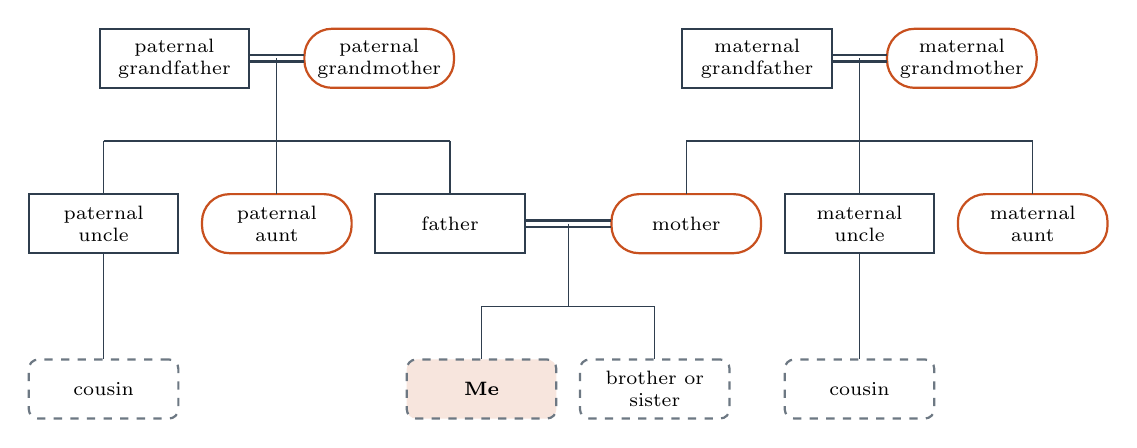
\begin{tikzpicture}[x=1cm,y=1cm]
\node[man]   (pgf) at (1.1,4.2)  {paternal\\grandfather};
\node[woman] (pgm) at (3.7,4.2)  {paternal\\grandmother};
\node[man]   (mgf) at (8.5,4.2)  {maternal\\grandfather};
\node[woman] (mgm) at (11.1,4.2) {maternal\\grandmother};
\node[man]   (pu) at (0.2,2.1)   {paternal\\uncle};
\node[woman] (pa) at (2.4,2.1)   {paternal\\aunt};
\node[man]   (fa) at (4.6,2.1)   {father};
\node[woman] (mo) at (7.6,2.1)   {mother};
\node[man]   (mu) at (9.8,2.1)   {maternal\\uncle};
\node[woman] (ma) at (12.0,2.1)  {maternal\\aunt};
\node[anyone] (c1) at (0.2,0)    {cousin};
\node[anyone,fill=ember!15] (me) at (5.0,0) {\textbf{Me}};
\node[anyone] (sb) at (7.2,0)    {brother or\\sister};
\node[anyone] (c2) at (9.8,0)    {cousin};
\draw[slate,thick] (2.05,4.24) -- (2.75,4.24);
\draw[slate,thick] (2.05,4.16) -- (2.75,4.16);
\draw[slate,thick] (9.45,4.24) -- (10.15,4.24);
\draw[slate,thick] (9.45,4.16) -- (10.15,4.16);
\draw[slate,thick] (5.55,2.14) -- (6.65,2.14);
\draw[slate,thick] (5.55,2.06) -- (6.65,2.06);
\draw[slate] (2.4,4.2) -- (2.4,3.15);
\draw[slate] (0.2,3.15) -- (4.6,3.15);
\draw[slate] (0.2,3.15) -- (0.2,2.48);
\draw[slate] (2.4,3.15) -- (2.4,2.48);
\draw[slate] (4.6,3.15) -- (4.6,2.48);
\draw[slate] (9.8,4.2) -- (9.8,3.15);
\draw[slate] (7.6,3.15) -- (12.0,3.15);
\draw[slate] (7.6,3.15) -- (7.6,2.48);
\draw[slate] (9.8,3.15) -- (9.8,2.48);
\draw[slate] (12.0,3.15) -- (12.0,2.48);
\draw[slate] (6.1,2.1) -- (6.1,1.05);
\draw[slate] (5.0,1.05) -- (7.2,1.05);
\draw[slate] (5.0,1.05) -- (5.0,0.38);
\draw[slate] (7.2,1.05) -- (7.2,0.38);
\draw[slate] (0.2,1.72) -- (0.2,0.38);
\draw[slate] (9.8,1.72) -- (9.8,0.38);
\end{tikzpicture}\par\nopagebreak\smallskip
{\small The family map, read from ``Me''. Square corners are men, rounded corners are women, dashed boxes can be either. A double line joins husband and wife, and the lines going down lead to their children.}
\end{center}

\infobox{Three habits that remove most mistakes}{
\begin{enumerate}
\item \textbf{Say it in words:} ``A is B's \dots''. The direction of the question is the first thing people get wrong.
\item \textbf{Draw a small tree.} A square for a man, a circle for a woman, a double line for a marriage, the children below.
\item \textbf{Name a relative only when you can:} the generation, the side and the sex of the person you name must all be known. If one is missing, the answer is a word with no sex (cousin, sibling) or ``cannot be determined''.
\end{enumerate}}

\subsection*{Spot-it table}
Read the wording, find the row, jump to the type.
\begin{center}\small\renewcommand{\arraystretch}{1.18}\setlength{\tabcolsep}{7pt}
\begin{tabularx}{\linewidth}{@{}>{\raggedright\arraybackslash}p{8.6cm} l >{\raggedright\arraybackslash}X@{}}
\toprule
\textbf{\color{slate}Wording in the question} & \textbf{\color{slate}Type} & \textbf{\color{slate}The one move} \\ \midrule
A is the father of B: how is B related to A & B1 & say it in words, then turn it round \\
A's mother's father's son: which generation & B2 & up $+1$, same $0$, down $-1$ \\
A's mother's brother's son & B3 & compress from the left \\
A's father's father's brother & B4 & each extra step up adds ``great'' \\
A is the cousin of B. B is the sister of C & B5 & is the sex given? \\
A boy points: ``His sister is my mother'' & B6 & work outward from the speaker \\
She is the daughter of my mother's only son & B7 & ``only son'' is me, if I am a man \\
A is the brother of B. B is the sister of C & B8 & join through the shared person \\
How is A's wife's brother related to A & B9 & a spouse's relatives are in-laws \\
A $+$ B means A is the mother of B & B10 & translate each symbol, then join \\
A family of six: P is the husband of Q & B11 & draw the tree \\
Counting boys and girls; fewest people & B12 & $b-1$ brothers; one person, two roles \\
\bottomrule
\end{tabularx}\end{center}

\subsection{B1. Family words and their opposites}
\spot ``A is the father of B. How is B related to A?'' ``P is the uncle of Q, and Q is a girl. How is Q related to P?''

\mech
\begin{enumerate}
\item ``How is A related to B?'' asks what A is to B. Say it in words first: ``A is B's \dots''. The family map at the start of the chapter shows the common words.
\item Turn it round for the opposite question. The word you need depends on the sex of the \emph{other} person (see the table).
\end{enumerate}
\begin{center}\small\renewcommand{\arraystretch}{1.18}\setlength{\tabcolsep}{8pt}
\begin{tabularx}{\linewidth}{@{}>{\raggedright\arraybackslash}X >{\raggedright\arraybackslash}X >{\raggedright\arraybackslash}X@{}}
\toprule
\textbf{\color{slate}A is B's \dots} & \textbf{\color{slate}B is a man: B is A's \dots} & \textbf{\color{slate}B is a woman: B is A's \dots} \\ \midrule
father or mother & son & daughter \\
son or daughter & father & mother \\
brother or sister & brother & sister \\
husband & (not possible) & wife \\
wife & husband & (not possible) \\
grandfather or grandmother & grandson & granddaughter \\
uncle or aunt & nephew & niece \\
nephew or niece & uncle & aunt \\
cousin & cousin & cousin \\
father-in-law or mother-in-law & son-in-law & daughter-in-law \\
son-in-law or daughter-in-law & father-in-law & mother-in-law \\
brother-in-law or sister-in-law & brother-in-law & sister-in-law \\
\bottomrule
\end{tabularx}\end{center}
\begin{enumerate}
\setcounter{enumi}{2}
\item If the sex of that other person is not given, the opposite word cannot be fixed (B5).
\end{enumerate}

\samp A is the father of B. B is a girl. How is B related to A?
\begin{enumerate}
\item B is A's \textbf{daughter}.
\end{enumerate}
\samp P is the uncle of Q. Q is a girl. How is Q related to P?
\begin{enumerate}
\item Q is P's \textbf{niece}.
\end{enumerate}
\samp A is B's grandmother. B is a boy. How is B related to A?
\begin{enumerate}
\item B is A's \textbf{grandson}.
\end{enumerate}

\tryit (a) M is N's mother, and N is a boy. How is N related to M? (b) X is Y's nephew, and Y is a woman. How is Y related to X? (c) S is T's brother-in-law, and T is a woman. How is T related to S?

\subsection{B2. Count the generations}
\spot ``A's mother's father's son.'' ``Is A's father's brother's son in A's own generation?''

\mech
\begin{enumerate}
\item Give every word a \textbf{level}: a parent is $+1$ (one generation up), a child is $-1$, and a brother, sister, husband, wife or cousin is $0$.
\item Add the levels along the chain. The total says which generation the person belongs to, compared with the start.
\item Then name the person by the side (father's or mother's) and the sex (B3).
\end{enumerate}
\begin{center}\small\renewcommand{\arraystretch}{1.18}\setlength{\tabcolsep}{8pt}
\begin{tabularx}{\linewidth}{@{}r >{\raggedright\arraybackslash}X@{}}
\toprule
\textbf{\color{slate}Level} & \textbf{\color{slate}Words} \\ \midrule
$+2$ & grandfather, grandmother, grand-uncle, grand-aunt (B4) \\
$+1$ & father, mother, uncle, aunt, father-in-law, mother-in-law \\
$0$ & brother, sister, cousin, husband, wife, brother-in-law, sister-in-law \\
$-1$ & son, daughter, nephew, niece, son-in-law, daughter-in-law \\
$-2$ & grandson, granddaughter, grandnephew, grandniece (B4) \\
\bottomrule
\end{tabularx}\end{center}

\samp A's mother's father's son.
\begin{enumerate}
\item $+1 + 1 - 1 = +1$: one generation up, on the mother's side.
\item The mother's father's son is the mother's brother: \textbf{maternal uncle}.
\end{enumerate}
\samp A's wife's father's son.
\begin{enumerate}
\item $0 + 1 - 1 = 0$: A's own generation, on the wife's side.
\item The wife's father's son is the wife's brother: \textbf{brother-in-law}.
\end{enumerate}
\samp A's father's father's wife.
\begin{enumerate}
\item $+1 + 1 + 0 = +2$: two generations up, on the father's side, a woman: \textbf{paternal grandmother}.
\end{enumerate}

\tryit (a) A's father's sister's son: which level, and which word? (b) Which of these is in A's own generation: father's sister, mother's brother's son, sister's daughter?

\subsection{B3. Chains: compress from the left}
\spot ``A's mother's brother's son.'' ``How is A related to B if B is A's father's sister's husband?''

\mech
\begin{enumerate}
\item Write the chain from the person it starts with: A $\to$ mother $\to$ brother $\to$ son.
\item Replace the first two links by one word from the table. Then combine that word with the next link. Repeat until one word is left.
\item The table below covers the blood relations (in-laws are in B9).
\end{enumerate}
\begin{center}\small\renewcommand{\arraystretch}{1.18}\setlength{\tabcolsep}{8pt}
\begin{tabularx}{\linewidth}{@{}>{\raggedright\arraybackslash}X >{\raggedright\arraybackslash}X@{}}
\toprule
\textbf{\color{slate}Chain from A} & \textbf{\color{slate}It is A's} \\ \midrule
father's father, mother's father & paternal grandfather, maternal grandfather \\
father's mother, mother's mother & paternal grandmother, maternal grandmother \\
father's brother, mother's brother & paternal uncle, maternal uncle \\
father's sister, mother's sister & paternal aunt, maternal aunt \\
father's or mother's sister's husband & uncle \\
father's or mother's brother's wife & aunt \\
uncle's or aunt's son or daughter & cousin \\
brother's or sister's son & nephew \\
brother's or sister's daughter & niece \\
son's or daughter's son & grandson \\
son's or daughter's daughter & granddaughter \\
father's or mother's son (not A himself) & brother \\
father's or mother's daughter (not A herself) & sister \\
\bottomrule
\end{tabularx}\end{center}
\begin{enumerate}
\setcounter{enumi}{3}
\item ``Father's son'' or ``mother's daughter'' means a brother or sister, not the person himself, unless it says ``only'' (B7).
\end{enumerate}

\samp A's mother's brother's son.
\begin{enumerate}
\item Mother's brother is the maternal uncle.
\item An uncle's son is a \textbf{cousin}.
\end{enumerate}
\samp A's father's sister's husband.
\begin{enumerate}
\item Father's sister is the paternal aunt.
\item An aunt's husband is an \textbf{uncle}.
\end{enumerate}
\samp B is A's mother's sister's husband, and A is a boy. How is A related to B?
\begin{enumerate}
\item Mother's sister is the maternal aunt, so B is A's uncle.
\item A is a boy, so A is B's \textbf{nephew}.
\end{enumerate}

\tryit (a) A's mother's mother's son. (b) B is A's brother's son, and A is a woman. How is A related to B? (c) A's father's sister's son's father.

\subsection{B4. Three or more steps: grand- and great-}
\spot ``A's father's father's brother.'' ``A's mother's mother's mother.'' ``A's brother's son's son.''

\mech
\begin{enumerate}
\item Count levels as in B2. A grandparent's generation is $+2$, a great-grandparent's $+3$; a grandchild's is $-2$, a great-grandchild's $-3$.
\item A parent of a grandparent is a \textbf{great-grandparent}. A grandparent's brother or sister is a \textbf{grand-uncle} or \textbf{grand-aunt} (also called great-uncle and great-aunt). A brother's or sister's grandchild is a \textbf{grandnephew} or \textbf{grandniece}. A grandchild's child is a \textbf{great-grandchild}.
\item Compress from the left as in B3 (table below).
\end{enumerate}
\begin{center}\small\renewcommand{\arraystretch}{1.18}\setlength{\tabcolsep}{9pt}
\begin{tabular}{@{}lll@{}}
\toprule
\textbf{\color{slate}Chain from A} & \textbf{\color{slate}It is A's} & \textbf{\color{slate}Level} \\ \midrule
father's father's father & great-grandfather & $+3$ \\
mother's mother's mother & great-grandmother & $+3$ \\
father's father's brother & grand-uncle & $+2$ \\
mother's mother's sister & grand-aunt & $+2$ \\
brother's son's son & grandnephew & $-2$ \\
sister's daughter's daughter & grandniece & $-2$ \\
son's son's son & great-grandson & $-3$ \\
daughter's daughter's daughter & great-granddaughter & $-3$ \\
\bottomrule
\end{tabular}\end{center}

\samp How is B related to A if B is the wife of A's father's father's father?
\begin{enumerate}
\item Father's father's father is the great-grandfather.
\item His wife is A's \textbf{great-grandmother}.
\end{enumerate}
\samp A's mother's mother's brother.
\begin{enumerate}
\item Mother's mother is the maternal grandmother.
\item Her brother is the maternal \textbf{grand-uncle}.
\end{enumerate}
\samp A's sister's son's daughter.
\begin{enumerate}
\item Sister's son is the nephew.
\item His daughter is A's \textbf{grandniece}.
\end{enumerate}

\tryit (a) A's father's mother's sister. (b) A's son's daughter's son. (c) B is A's grandniece, and A is a man. How is A related to B?

\subsection{B5. Words with no sex, and ``cannot be determined''}
\spot ``A is the cousin of B. B is the sister of C. How is A related to C?'' ``A is the child of B. B is the father of C.''

\mech
\begin{enumerate}
\item Some family words give a sex and some do not (table below).
\end{enumerate}
\begin{center}\small\renewcommand{\arraystretch}{1.18}\setlength{\tabcolsep}{7pt}
\begin{tabularx}{\linewidth}{@{}>{\raggedright\arraybackslash}X >{\raggedright\arraybackslash}X >{\raggedright\arraybackslash}X@{}}
\toprule
\textbf{\color{slate}Gives a man} & \textbf{\color{slate}Gives a woman} & \textbf{\color{slate}Gives no sex} \\ \midrule
father, son, brother, husband, uncle, nephew, grandfather, grandson, father-in-law, son-in-law, brother-in-law & mother, daughter, sister, wife, aunt, niece, grandmother, granddaughter, mother-in-law, daughter-in-law, sister-in-law & cousin, sibling, child, parent, spouse, grandchild, grandparent, friend, relative \\
\bottomrule
\end{tabularx}\end{center}
\begin{enumerate}
\setcounter{enumi}{1}
\item A person's sex is known only from a clue: a gendered word used for them (``A is the brother of B''), a pronoun (he, she), or a description (a boy, a woman). A name alone is not a clue. (Some books treat common names as men or women; follow your book if it does.)
\item Use a gendered word in the answer only if the sex of the person you name is known. If it is not, give the word with no sex, or say ``cannot be determined'' when every option is gendered.
\item Brothers and sisters share their relatives: if A is the cousin of B and C is B's brother or sister, A is C's cousin too.
\end{enumerate}

\samp A is the cousin of B. B is the sister of C. How is A related to C?
\begin{enumerate}
\item B and C are brother and sister, so they share their relatives: A is C's \textbf{cousin}.
\item ``Cousin'' gives no sex, which is fine.
\end{enumerate}
\samp A is the child of B. B is the father of C. How is A related to C?
\begin{enumerate}
\item A and C are both B's children: \textbf{siblings}.
\item A's sex is not given, so ``brother'' or ``sister'' cannot be chosen.
\item With only gendered options the answer is ``cannot be determined''.
\end{enumerate}
\samp A is the brother of B. B is the husband of C. How is A related to C?
\begin{enumerate}
\item A is the brother of C's husband: C's \textbf{brother-in-law}.
\item The word ``brother'' gives A's sex, and that is all this answer needs.
\end{enumerate}

\tryit (a) P is the spouse of Q. R is the mother of P. How is R related to Q? (b) X is the sibling of Y. Z is the daughter of X. How is Y related to Z?

\subsection{B6. Pointing at someone}
\spot ``A man, pointing to another man, says: `His mother is the only daughter of my mother.' How is the pointed man related to the speaker?''

\mech
\begin{enumerate}
\item Start with the speaker: ``I'', ``my'' and ``me'' are the speaker. The person pointed at is the one asked about.
\item Work outward from the speaker, replacing each piece of the sentence by one word (B3). ``The only daughter of my mother'' is my sister (or me, if I am a woman: B7).
\item Join the pieces until the person pointed at is tied to the speaker. The answer is what that person is \emph{to the speaker}.
\end{enumerate}

\samp A man, pointing to another man, says: ``His mother is the only daughter of my mother.''
\begin{enumerate}
\item The only daughter of my mother is my sister.
\item His mother is my sister, so he is my sister's son: my \textbf{nephew}.
\end{enumerate}
\samp A girl, pointing to a woman, says: ``Her husband is the brother of my father.''
\begin{enumerate}
\item My father's brother is my paternal uncle, and the woman is his wife: my \textbf{aunt}.
\end{enumerate}
\samp A boy, pointing to a man, says: ``His sister is my mother.''
\begin{enumerate}
\item The man's sister is the boy's mother, so the man is the mother's brother: my \textbf{maternal uncle}.
\end{enumerate}

\tryit (a) A boy, pointing to a girl, says: ``She is the daughter of my mother's brother.'' (b) A girl, pointing to a man, says: ``He is the husband of my mother's mother.''

\subsection{B7. ``My \dots only \dots'': the self-reference trick}
\spot ``She is the daughter of the only son of my mother.'' ``He is the son of my father's only son.''

\mech
\begin{enumerate}
\item ``The only son of my mother (or father)'' is \textbf{me} if I am a man. If I am a woman it is my \textbf{brother}.
\item ``The only daughter of my mother (or father)'' is \textbf{me} if I am a woman. If I am a man it is my \textbf{sister}.
\item Replace the phrase by ``I'' or by the brother or sister, then carry on as in B6. The speaker's sex must be given (a man, a woman, a boy, a girl).
\item Without ``only'', ``my father's son'' means a brother (B3).
\end{enumerate}

\samp A man, pointing to a girl, says: ``She is the daughter of the only son of my mother.''
\begin{enumerate}
\item I am a man, so the only son of my mother is me.
\item She is my \textbf{daughter}.
\end{enumerate}
\samp A woman, pointing to a boy, says: ``He is the son of my mother's only daughter.''
\begin{enumerate}
\item I am a woman, so my mother's only daughter is me.
\item He is my \textbf{son}.
\end{enumerate}
\samp A woman, pointing to a man, says: ``He is the son of my father's only son.''
\begin{enumerate}
\item I am a woman, so my father's only son is my brother.
\item The man is my brother's son: my \textbf{nephew}.
\end{enumerate}

\tryit (a) A man, pointing to a girl, says: ``She is the daughter of my father's only son.'' (b) A woman, pointing to a man, says: ``He is the only son of my mother's only son.'' (c) A man, pointing to a woman, says: ``She is the mother of my mother's only daughter.''

\subsection{B8. Statements about different people}
\spot ``A is the brother of B. B is the sister of C. C is the father of D. How is A related to D?''

\mech
\begin{enumerate}
\item Write each statement as a link and mark every sex a word gives: brother, father, husband, son mean a man; sister, mother, wife, daughter mean a woman.
\item Join the statements through the shared person. Statements about brothers and sisters put all of them in one set of siblings, who share every relative.
\item Compress the chain from the first person to the last (B3) and name the answer by the sex of the first person.
\end{enumerate}

\begin{center}
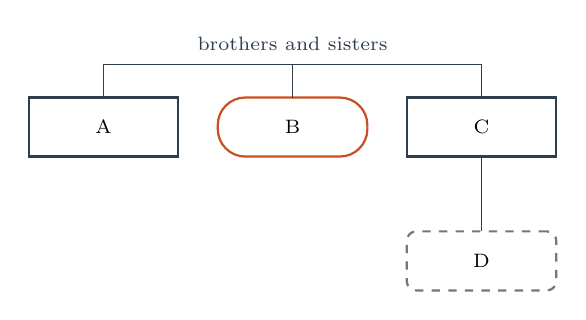
\begin{tikzpicture}[x=1cm,y=1cm]
\node[man]    (a) at (0,1.7)   {A};
\node[woman]  (b) at (2.4,1.7) {B};
\node[man]    (c) at (4.8,1.7) {C};
\node[anyone] (d) at (4.8,0)   {D};
\draw[slate] (0,2.075) -- (0,2.5) -- (4.8,2.5) -- (4.8,2.075);
\draw[slate] (2.4,2.075) -- (2.4,2.5);
\node[slate,font=\scriptsize,anchor=south] at (2.4,2.55) {brothers and sisters};
\draw[slate] (4.8,1.325) -- (4.8,0.375);
\end{tikzpicture}\par\nopagebreak\smallskip
{\small A, B and C are brothers and sisters. C is D's father, so A (a man) is D's father's brother.}
\end{center}

\samp A is the brother of B. B is the sister of C. C is the father of D. How is A related to D?
\begin{enumerate}
\item A, B and C are brothers and sisters.
\item A is a man, so A is C's brother, and C is D's father: A is D's \textbf{paternal uncle}.
\end{enumerate}
\samp P is the mother of Q. Q is the sister of R. R is the husband of S. How is P related to S?
\begin{enumerate}
\item Q and R are brother and sister, so P is also R's mother.
\item R is S's husband: P is S's \textbf{mother-in-law}.
\end{enumerate}
\samp X is the daughter of Y. Y is the sister of Z. Z is the father of W. How is X related to W?
\begin{enumerate}
\item Y is the sister of W's father, so Y is W's paternal aunt.
\item X is her daughter: W's \textbf{cousin}.
\end{enumerate}

\tryit (a) A is the father of B. B is the brother of C. C is the mother of D. How is A related to D? (b) P is the wife of Q. Q is the son of R. R is the mother of S. How is P related to S?

\subsection{B9. In-laws and marriage}
\spot ``A's wife's brother.'' ``B is the husband of A's sister.'' ``How is the father of A's wife related to A?''

\mech
\begin{enumerate}
\item Your spouse's relatives are your \textbf{in-laws}: father-in-law, mother-in-law, brother-in-law, sister-in-law.
\item Your brother's or sister's spouse is an in-law too, and so is your child's spouse.
\item The in-law word is used for one step only. After that the ordinary words return: your wife's brother's son is your nephew.
\end{enumerate}
\begin{center}\small\renewcommand{\arraystretch}{1.18}\setlength{\tabcolsep}{8pt}
\begin{tabularx}{\linewidth}{@{}>{\raggedright\arraybackslash}X >{\raggedright\arraybackslash}X@{}}
\toprule
\textbf{\color{slate}Chain from A} & \textbf{\color{slate}It is A's} \\ \midrule
wife's or husband's father & father-in-law \\
wife's or husband's mother & mother-in-law \\
wife's or husband's brother; sister's husband & brother-in-law \\
wife's or husband's sister; brother's wife & sister-in-law \\
son's wife & daughter-in-law \\
daughter's husband & son-in-law \\
wife's or husband's brother's son & nephew \\
wife's or husband's sister's daughter & niece \\
\bottomrule
\end{tabularx}\end{center}

\samp A's wife's brother. A's sister's husband.
\begin{enumerate}
\item Both are A's \textbf{brother-in-law}: one is the wife's brother, the other the sister's husband.
\end{enumerate}
\samp How is the father of A's wife related to A?
\begin{enumerate}
\item He is A's \textbf{father-in-law}.
\end{enumerate}
\samp A's wife's brother's son.
\begin{enumerate}
\item The wife's brother is a brother-in-law.
\item After that one step the ordinary word returns: his son is A's \textbf{nephew}.
\end{enumerate}
\samp B is the husband of A's sister, and A is a woman. How is A related to B?
\begin{enumerate}
\item A's sister is B's wife, so A is the sister of B's wife: B's \textbf{sister-in-law}.
\end{enumerate}

\tryit (a) How is a woman's husband's mother's husband related to her? (b) A is a woman and B is her son's wife. How is A related to B? (c) A is a man and B is the sister of A's wife. How is A related to B?

\subsection{B10. Coded relations}
\spot ``A $+$ B means A is the mother of B; A $-$ B means A is the brother of B; A $\times$ B means A is the father of B; A $\div$ B means A is the sister of B. What does P $\times$ Q $-$ R mean?''

\mech
\begin{enumerate}
\item Write the meaning of each symbol and note the sex it gives to the \emph{left} letter: here $+$ and $\div$ make the left letter a woman, $\times$ and $-$ make it a man.
\item Translate each pair of neighbouring letters: P $\times$ Q is ``P is the father of Q'', and Q $-$ R is ``Q is the brother of R''. The middle letter joins them (B8).
\item Name the first letter's relation to the last. To find the expression for a given relation, build the chain from the last letter backwards.
\end{enumerate}

\samp P $\times$ Q $-$ R, with the codes above.
\begin{enumerate}
\item P is the father of Q, and Q is the brother of R.
\item Q and R are siblings, so P is also R's father: \textbf{P is the father of R}.
\end{enumerate}
\samp A $+$ B $\times$ C.
\begin{enumerate}
\item A is the mother of B, and B is the father of C: A is the mother of C's father, so A is C's \textbf{paternal grandmother}.
\end{enumerate}
\samp Which expression shows that P is the maternal uncle of R?
\begin{enumerate}
\item A maternal uncle is the mother's brother: P is the brother of Q, and Q is the mother of R.
\item The expression is \textbf{P $-$ Q $+$ R}.
\end{enumerate}
\samp M $\div$ N $\times$ O.
\begin{enumerate}
\item M is the sister of N, and N is the father of O: M is the sister of O's father, so O's \textbf{paternal aunt}.
\end{enumerate}

\tryit Codes: A \$ B means A is the brother of B; A \# B means A is the mother of B; A @ B means A is the daughter of B. What does each mean? (a) P \# Q \$ R. (b) P @ Q \# R. (c) P \$ Q @ R.

\subsection{B11. Family puzzles with a tree}
\spot ``P, Q, R, S, T and U belong to one family. P is the husband of Q. Q is the mother of R and S. \dots''

\mech
\begin{enumerate}
\item Draw generations as rows, oldest at the top. A square is a man, a circle a woman, a double line joins husband and wife, and the children hang below the couple.
\item Mark each sex as soon as a word gives it. Add one statement at a time. Add an unnamed person only when a statement forces one (for example a father who is not named).
\item Exam convention: the children of a married couple are the couple's own children, and all the people named are different.
\item Read the answers off the finished tree. If two different trees fit the statements and give different answers, the answer is ``cannot be determined''.
\end{enumerate}

\begin{center}
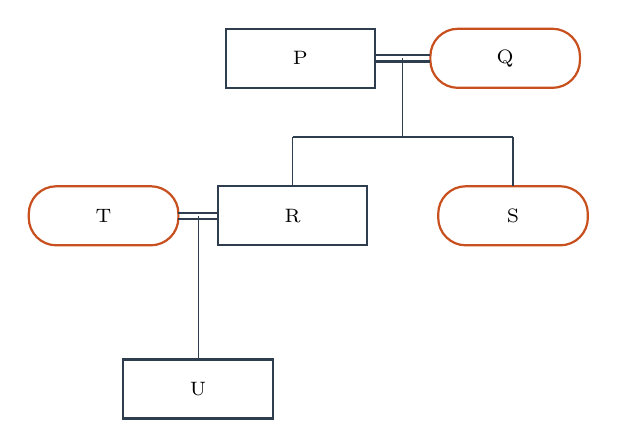
\begin{tikzpicture}[x=1cm,y=1cm]
\node[man]   (p) at (2.7,4.2) {P};
\node[woman] (q) at (5.3,4.2) {Q};
\node[woman] (t) at (0.2,2.2) {T};
\node[man]   (r) at (2.6,2.2) {R};
\node[woman] (s) at (5.4,2.2) {S};
\node[man]   (u) at (1.4,0)   {U};
\draw[slate,thick] (3.65,4.24) -- (4.35,4.24);
\draw[slate,thick] (3.65,4.16) -- (4.35,4.16);
\draw[slate,thick] (1.15,2.24) -- (1.65,2.24);
\draw[slate,thick] (1.15,2.16) -- (1.65,2.16);
\draw[slate] (4.0,4.2) -- (4.0,3.2);
\draw[slate] (2.6,3.2) -- (5.4,3.2);
\draw[slate] (2.6,3.2) -- (2.6,2.575);
\draw[slate] (5.4,3.2) -- (5.4,2.575);
\draw[slate] (1.4,2.2) -- (1.4,0.375);
\end{tikzpicture}\par\nopagebreak\smallskip
{\small The tree for the first puzzle below. P and Q are the couple at the top; R and S are their children; T is R's wife; U is their son.}
\end{center}

\samp P, Q, R, S, T and U are members of one family. P is the husband of Q. Q is the mother of R and S. R is a man and S is a woman. T is the wife of R, and U is their son. (a) How is P related to U? (b) How is S related to U?
\begin{enumerate}
\item (a) P is the father of R, and R is U's father: P is U's \textbf{paternal grandfather}.
\item (b) S is R's sister, and R is U's father: S is U's \textbf{paternal aunt}.
\end{enumerate}
\samp P is the mother of Q. R is the sibling of Q. S is the child of R. (a) How is P related to S? (b) How is Q related to S?
\begin{enumerate}
\item (a) P is the mother of Q and R, and S is R's child: P is S's \textbf{grandmother}.
\item Whether paternal or maternal cannot be told, because R's sex is not given.
\item (b) Q is a brother or sister of S's parent: an uncle or an aunt.
\item Q's sex is not given, so \textbf{cannot be determined}.
\end{enumerate}
\samp A is the father of B. B is the sister of C. C is the husband of D. E is the mother of D. F is the brother of E. (a) How is E related to C? (b) How is F related to D?
\begin{enumerate}
\item (a) E is the mother of C's wife: C's \textbf{mother-in-law}.
\item (The first statement is not needed.)
\item (b) F is the brother of D's mother: D's \textbf{maternal uncle}.
\end{enumerate}

\tryit A is the wife of B. C and F are their sons. D is the wife of C. E is the daughter of C and D. (a) How is A related to E? (b) How is F related to E? (c) How is B related to D?

\subsection{B12. Counting children, and one person in two roles}
\spot ``Each girl in a family has as many brothers as sisters, and each boy has twice as many sisters as brothers. How many children?'' ``Two fathers and two sons: what is the fewest number of people?''

\mech
\begin{enumerate}
\item Let there be $b$ boys and $g$ girls. A boy is not his own brother, and a girl is not her own sister (table below).
\end{enumerate}
\begin{center}\small\renewcommand{\arraystretch}{1.18}\setlength{\tabcolsep}{12pt}
\begin{tabular}{@{}lll@{}}
\toprule
 & \textbf{\color{slate}brothers} & \textbf{\color{slate}sisters} \\ \midrule
\textbf{\color{slate}a boy has} & $b - 1$ & $g$ \\
\textbf{\color{slate}a girl has} & $b$ & $g - 1$ \\
\bottomrule
\end{tabular}\end{center}
\begin{enumerate}
\setcounter{enumi}{1}
\item Turn each sentence into an equation with these two lines and solve. The family has $b + g$ children.
\item One person can fill two roles: the middle generation is both a father and a son. So the fewest people are found by drawing the shortest chain (figure below).
\end{enumerate}

\begin{center}
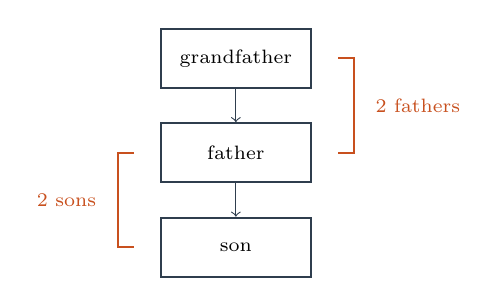
\begin{tikzpicture}[x=1cm,y=1cm]
\node[man] (g) at (0,2.4) {grandfather};
\node[man] (f) at (0,1.2) {father};
\node[man] (s) at (0,0)   {son};
\draw[->,slate] (g.south) -- (f.north);
\draw[->,slate] (f.south) -- (s.north);
\draw[ember,thick] (1.3,2.4) -- (1.5,2.4) -- (1.5,1.2) -- (1.3,1.2);
\node[ember,font=\scriptsize,anchor=west] at (1.65,1.8) {2 fathers};
\draw[ember,thick] (-1.3,1.2) -- (-1.5,1.2) -- (-1.5,0) -- (-1.3,0);
\node[ember,font=\scriptsize,anchor=east] at (-1.65,0.6) {2 sons};
\end{tikzpicture}\par\nopagebreak\smallskip
{\small Three people are enough: the middle one is both a father and a son.}
\end{center}

\samp Each girl has as many brothers as sisters, and each boy has twice as many sisters as brothers. How many children?
\begin{enumerate}
\item Girl: $b = g - 1$.
\item Boy: $g = 2(b - 1)$.
\item Put $g = b + 1$ into the second: $b + 1 = 2b - 2$, so $b = 3$ and $g = 4$. \textbf{7} children.
\end{enumerate}
\samp A man has 3 daughters, and each daughter has exactly one brother. How many children?
\begin{enumerate}
\item A girl has $b$ brothers, so $b = 1$: one son and three daughters, \textbf{4} children.
\end{enumerate}
\samp Two fathers and two sons: what is the fewest number of people?
\begin{enumerate}
\item A grandfather, his son and his grandson: the middle one is a father and a son. \textbf{3} people.
\end{enumerate}

\tryit (a) Each boy has three times as many sisters as brothers, and each girl has as many brothers as sisters. How many children? (b) Rita has 3 brothers and 2 sisters. How many sisters does each of her brothers have? (c) Two mothers and two daughters: what is the fewest number of people?

\subsection*{Shortcuts to memorise}
\begin{center}\small\renewcommand{\arraystretch}{1.9}\setlength{\tabcolsep}{8pt}
\begin{tabularx}{\linewidth}{@{}>{\raggedright\arraybackslash}X>{\raggedright\arraybackslash}X@{}}
\toprule
\textbf{\color{slate}Idea} & \textbf{\color{slate}Rule} \\ \midrule
The question & ``How is A related to B?'' means ``A is B's \dots''; say it in words first \\
Levels & up to a parent $+1$, sideways $0$, down to a child $-1$; add them along the chain \\
Naming & level, side (father's or mother's) and the sex of the person you name \\
Parent's brother, sister & paternal or maternal uncle, aunt \\
Child of an uncle or aunt & cousin (no sex word) \\
Child of a brother or sister & nephew (boy), niece (girl) \\
Spouse's relatives, sibling's spouse & in-laws, for one step only \\
``Father's son'', ``mother's daughter'' & brother, sister \\
``My mother's only son'' & me if I am a man, my brother if I am a woman \\
``My mother's only daughter'' & me if I am a woman, my sister if I am a man \\
A sex & known only from a clue, never from a name alone \\
Brothers and sisters & share every relative \\
Coded relation & translate each symbol, join through the shared letter \\
Boys and girls & a boy has $b-1$ brothers and $g$ sisters; a girl has $b$ brothers and $g-1$ sisters \\
One person, two roles & the middle generation is both a parent and a child \\
Great and grand & each extra step above grand- adds ``great'' \\
\bottomrule
\end{tabularx}\end{center}

\subsection*{Sanity checks before you mark the option}
\infobox{Ten seconds that save a wrong answer}{
\begin{itemize}
\item Did you answer for the right direction: what A is to B, not what B is to A?
\item Does every sex word in your answer come from a clue in the question?
\item Does the level fit: the parents' generation, the same generation, or the children's?
\item If two trees fit the statements and give different answers, is your answer ``cannot be determined''?
\item Did you use only the people and marriages the statements give?
\end{itemize}}

\subsection*{Traps}
\begin{enumerate}
\item \textbf{Answering backwards.} ``How is A related to B?'' asks what A is to B (B1).
\item \textbf{Naming a sex the question never gives}, for example ``uncle'' for a sibling of unknown sex (B5).
\item \textbf{Mixing the sides.} Father's brother is the paternal uncle, mother's brother the maternal uncle (B3).
\item \textbf{Calling the child of an uncle or aunt a nephew or niece.} It is a cousin (B3).
\item \textbf{Reading ``the only son of my mother'' as my brother when I am a man.} It is me (B7).
\item \textbf{Counting a child as his or her own brother or sister} in boys-and-girls puzzles (B12): a boy has $b-1$ brothers.
\item \textbf{Forgetting that brothers and sisters share relatives} (B5, B8).
\item \textbf{Keeping ``in-law'' for every step} (B9): the wife's brother is a brother-in-law, but his son is a nephew.
\item \textbf{Reading a coded relation from the wrong end} (B10): a symbol between two letters describes the left letter.
\item \textbf{Adding a person the statements do not mention}, such as an extra marriage or child, when drawing the tree (B11).
\item \textbf{Treating great- and grand- as the same level} (B4): a great-grandparent is three levels up.
\item \textbf{Adding levels with the wrong signs} (B2): up is $+$, down is $-$.
\end{enumerate}

\subsection*{Answers to ``Try it''}
\begin{center}\small\renewcommand{\arraystretch}{1.2}\setlength{\tabcolsep}{8pt}
\begin{tabularx}{\linewidth}{@{}l>{\raggedright\arraybackslash}X>{\raggedright\arraybackslash}X@{}}
\toprule
\textbf{\color{slate}Type} & \textbf{\color{slate}Answer} & \textbf{\color{slate}Working} \\ \midrule
B1 & (a) son \newline (b) aunt \newline (c) sister-in-law & (a) N is a boy \newline (b) Y is a woman, and the opposite of nephew is uncle or aunt \newline (c) T is a woman \\
B2 & (a) level 0, cousin \newline (b) mother's brother's son & (a) $+1 + 0 - 1 = 0$, an aunt's son \newline (b) aunt $+1$, cousin $0$, niece $-1$ \\
B3 & (a) maternal uncle \newline (b) aunt (paternal) \newline (c) uncle & (a) mother's mother's son is the mother's brother \newline (b) A is B's father's sister \newline (c) father's sister is an aunt, her son a cousin, his father the aunt's husband, an uncle \\
B4 & (a) paternal grand-aunt \newline (b) great-grandson \newline (c) grand-uncle & (a) father's mother is the paternal grandmother, and this is her sister \newline (b) son's daughter is a granddaughter, her son is a great-grandson \newline (c) A is the brother of B's grandparent \\
B5 & (a) mother-in-law \newline (b) uncle or aunt, cannot be determined & (a) R is a woman and the mother of Q's spouse \newline (b) Y's sex is not given \\
B6 & (a) cousin \newline (b) maternal grandfather & (a) mother's brother's daughter \newline (b) mother's mother's husband \\
B7 & (a) daughter \newline (b) nephew \newline (c) mother & (a) my father's only son is me \newline (b) a woman's mother's only son is her brother, and the man is his only son \newline (c) my mother's only daughter is my sister, and her mother is my mother \\
B8 & (a) maternal grandfather \newline (b) sister-in-law & (a) A is also C's father, and C is D's mother \newline (b) Q and S are siblings, so P is the wife of S's brother \\
B9 & (a) father-in-law \newline (b) mother-in-law \newline (c) brother-in-law & (a) her husband's mother's husband is her husband's father \newline (b) A is the mother of B's husband \newline (c) A is the husband of B's sister \\
B10 & (a) P is the mother of R \newline (b) P is the sister of R \newline (c) P is the son of R & (a) P is Q's mother and Q is R's brother \newline (b) P and R are both Q's children and P is a daughter \newline (c) P is Q's brother and Q is R's daughter \\
B11 & (a) paternal grandmother \newline (b) paternal uncle \newline (c) father-in-law & (a) A is the mother of C, who is E's father \newline (b) F is the brother of E's father C \newline (c) B is the father of C, D's husband \\
B12 & (a) 5 children \newline (b) 3 \newline (c) 3 & (a) $g = 3(b - 1)$ and $b = g - 1$, so $b = 2$ and $g = 3$ \newline (b) Rita is a girl, so $b = 3$ and $g - 1 = 2$, $g = 3$: each brother has all three girls as sisters \newline (c) grandmother, mother, daughter \\
\bottomrule
\end{tabularx}\end{center}

\end{document}
